%%%%%%%%%%%%%%%%%%%%%%%%%%%%%%%%%%%%%%%%%%%%%%%%%%%%%%%%%%%%%%%%%%%%%%%%%%%%%%%%
%\documentclass[12pt,papel,twoside]{ibtesis}
\documentclass{ibtesis}

% \documentclass[12pt,papel,singlespace,oneside]{ibtesis}
% \documentclass[12pt,papel,preprint,singlespace,oneside]{ibtesis}

%%%%%%%%%%%%%%%%%%%%% Paquetes extra %%%%%%%%%%%%%%%%%%%%%%%%%%%%%%%%%%%%%%%%%%%
% Por conveniencia: aqu\'{\i} puede cargar todos los paquetes y definir los comandos 
% que necesite
\usepackage{ibextra}
\usepackage[utf8]{inputenc}
\usepackage{subcaption}  % Enable figure captions or figure notes
\usepackage{float}
\usepackage{nicefrac}
\usepackage{mathtools}
\usepackage{textcomp}

\usepackage{amsfonts}

\newcommand{\done}{\item[\checkmark]}
%%%%%%%%%%%%%%%%%%%%%%%%%%%%%%%%%%%%%%%%%%%%%%%%%%%%%%%%%%%%%%%%%%%%%%%%%%%%%%%%
%%%%%%%%%%%%%%%%%%%%% Informacion sobre la tesis %%%%%%%%%%%%%%%%%%%%%%%%%%%%%%%
\title{Análisis de las direcciones de arribo de rayos cósmicos de ultra-alta energía en el Observatorio Pierre Auger}
\author{Evelyn~G.~Coronel}
\director{Dra.~Silvia Mollerach}
%\codirector{Dr.~J.~Otro m\'{a}s}b
\carrera{Tesis de Maestría en Ciencias F\'{\i}sicas}
\grado{Maestrando}
\laboratorio{Partículas y Campos -- Centro At\'{o}mico Bariloche}
\jurado{Dr.~Diego~Harari (Instituto Balseiro)}

\palabrasclave{Rayos Cósmicos, Análisis de datos, Instituto Balseiro}
%\keywords{Cosmic Rays, Data Analysis, Balseiro Institute}
\neembaeguasu{Mba'e michĩ yvágagui ouva, Mbo'ehaoguasu Balseiro}
% Si queremos poner la fecha manualmente:
% \date{Diciembre de 2099}

%%%%%%%%%%%%%%%%%%%%%%%%%%%%%%%%%%%%%%%%%%%%%%%%%%%%%%%%%%%%%%%%%%%%%%%%%%%%%%%%
%\titlepagefalse % Si no quiere compilar la portada descomente esta linea
%\includeonly{apendices} % Compilar s\'{o}lo estos archivos 
%\graphicspath{{/h}} % Lugar donde encontrar las figuras generales (se puede poner uno en cada cap{\'{\i}}tulo)
%%%%%%%%%%%%%%%%%%%%%%%%%%%%%%%%%%%%%%%%%%%%%%%%%%%%%%%%%%%%%%%%%%%%%%%%%%%%%%%%


%\setcounter{tocdepth}{4}
%\setcounter{secnumdepth}{4}
\begin{document}

\begin{preliminary}

%%% \'{I}ndices %%%%

\begin{abreviaturas}

\begin{tabular}{l l}
CR: 		& Rayos cósmicos  (\emph{Cosmic Rays}) \\
CMB: 		& Radiación Cósmica de Fondo (\emph{Cosmic Microwave Background})\\
FD: 		& Detector de Fluorescencia (\emph{Fluorescence Detector}) \\
SD: 		& Detector de Superficie (\emph{Surface Detector})  \\
WCD: 		& Detector de radiación Cherenkov de agua\\
EAS: 		& Lluvia Atmosférica Extendida  (\emph{Extensive Air Shower})    \\
VAOD: 		& Profundidad atmosférica óptica vertical (\emph{Vertical Atmosferic Optical Depth})\\
CLF:		& \emph{Central Laser Facility}\\
XLF:		& \emph{eXtreme Laser Facility}\\
X$_{max}$: 	& Profundidad atmosférica del máximo de la lluvia \\
LDF: 		& Función de Distribución Lateral (\emph{Lateral Distribution Function}) \\
S(1000): 	& Señal a 1000\,m del núcleo de la lluvia y al nivel del suelo \\
S(1000)$_w$:& Señal de S(1000) corregida por la modulación del clima. \\
CIC: 		& Corte de Intensidad Constante (\emph{Constant Intensity Cut}) \\
S$_{38}$: 	& Señal a 1000\,m del núcleo y al nivel del suelo si el ángulo cenital del evento fuera de $38^o$\\
S$_{38,w}$: & Señal S$_{38}$ corregida por la modulación del clima \\
eV: 		& electrón Voltio, $1\,$eV$= 1.602\times 10^{-19}\,$J \\
EeV: 		& $1\,$EeV$=10^{18}\,$eV\\
PMT: 		& Tubo fotomultiplicador (\emph{Photo-Multiplier Tube})\\
VEM: 		& Muón vertical equivalente (\emph{Vertical Equivalent Muon})\\
ICRC: 		& Conferencia Internacional de Rayos Cósmicos (\emph{International Cosmic Ray Conference})\\
\end{tabular}
                     %Abreviaturas
\end{abreviaturas}

	\tableofcontents                %\'{I}ndice
	\listoffigures                  %Figuras
	%\listoftables                   %Tablas

	\begin{resumen}%
Cuando un rayo cósmico interactúa con una molécula en la parte superior de la atmósfera, se inicia un proceso en el cual se generan otras partículas secundarias. Este proceso es conocido como lluvia atmosférica extendida. Estas lluvias pueden ser detectadas sobre la superficie de la Tierra mediante varios experimentos. Este trabajo utiliza los datos recolectados por los detectores de superficie separados en 1500\,m entre sí del Observatorio Pierre Auger durante los años 2005-2020. 

Se estudian eventos obtenidos mediante distintos algoritmos de adquisición de datos. El \emph{Disparo Estándar} que alcanza eficiencia completa para eventos asociados a rayos cósmicos de energía mayor a $3\,$EeV, y el \emph{Todos los Disparos} llega a detectar, con una eficiencia del 100\%, eventos por encima de $1\,$EeV. El primer disparo contiene eventos registrados desde el año 2005 y el segundo disparo empezó funcionar desde el 2013. 

Las condiciones atmosféricas como la presión (P), la temperatura (T) y la densidad ($\rho \propto \nicefrac{P}{T}$) afectan el desarrollo de la lluvia a través de la atmósfera. Las variaciones de estas condiciones inducen una modulación en la señal producida en los detectores por un rayo cósmico de una dada energía. Mediante un estudio hecho por la Colaboración sobre eventos del Disparo Estándar, se corrigió el efecto de esta modulación en la estimación de la energía de los rayos cósmicos medidos por el Observatorio. En este trabajo extendimos el periodo de tiempo analizado de esta modulación, y se observó que los parámetros obtenidos son comparables con la reconstrucción oficial. También se estudia la modulación en los datos de Todos los Disparos, y se realiza una corrección sobre el mismo conjunto de datos usando los parámetros obtenidos por este trabajo.

Se  estudian las modulaciones en distintas frecuencias mediante el análisis en Rayleigh, y se propone una variable generalizada para hacer un barrido en frecuencias con el método de East-West. Se obtienen resultados de la modulación en ascensión recta para distintos rangos de energía y se comparan con resultados reportados por la Colaboración Pierre Auger.

\end{resumen}


% \begin{nemombyky}%
% Mbyjakua\'ape (\emph{astronomía} karaiñe'\~eme) ojeikuaase mba\textquotesingle e oik\'ova umi mba\textquotesingle e  michĩ yv\'agagui o\'uva (\emph{rayos cósmicos} karaiñe'\~eme) oguah\~evove amo yvatetépe (\emph{atmósfera} karaiñe'\~eme). Ombok\'aramo tuminguaave\textquotesingle \~yty (\emph{conjunto de átomos o molécula}  karaiñe'\~eme ) yvatetépe oĩva, oñepyr\~u ojapo het\~a umi tuminguaave\textquotesingle \~yjokaku\'era (\emph{partículas}  karaiñe'\~eme ) op\'arupi. Ko\textquotesingle a       ha\textquotesingle e  h\'ina peteĩ ama guasu tuminguaave\textquotesingle \~yjoka rehegua ( \emph{lluvia atmosf\'erica extendida} karaiñe'\~eme). Umi ama guasuku\'era tuichaterei ha ikatu eñeña\textquotesingle ã yvy ári op\'arupi. Mend\'osape oĩ peteĩ mba\textquotesingle etuicha h\'erava \emph{Pierre Auger} Mbyjañama\textquotesingle \~eha\~gua (\emph{Observatorio Pierre Auger}) oña'\~ava ko ama. Ko\textquotesingle  ape romba\textquotesingle  ap\'ota umi ama ko mbyjañama\textquotesingle \~eha\~gua oña\textquotesingle \~ava\textquotesingle  kue 2005-guive 2018-peve. Mba\textquotesingle \'eichapa umi amaku\'era oguah\~e yvy \'ari ikatu ojuavy hakúramo (T, \emph{temperatura} karaiñe\textquotesingle \~eme) tér\~a  poh\'yiramo pe pytundyry mbyjañama\textquotesingle \~eha\~gua áripe ($\rho$, \emph{densidad} h\'erava karaiñe\textquotesingle \~eme). Ko mbyjañama'\~eha\~gua ojapova\textquotesingle ekue peteĩ tembiapo ha ko\textquotesingle ape rojapojey up\'eva roikuaaha\~gua umi papapo oñenoh\~eva\textquotesingle ekue oiko gueteri ko'\~anga peve, ha rotopa kóva oikópa añetete.
% \end{nemombyky}



%%% Local Variables: 
%%% mode: latex
%%% TeX-master: "template"
%%% End: 


\end{preliminary}

%Podemos usar cualquiera de los dos comandos: \input o \include para incluir el texto
	

\chapterquote{We can only measure what Nature sends us}{Jim Cronin}  

Desde el descubrimiento de los rayos cósmicos en 1911 por Victor Hess, numerosos experimentos han intentado caracterizarlos. A partir del 2004, el Observatorio Pierre Auger ha detectado rayos cósmicos con el objetivo de estudiar su origen. Un análisis adecuado de los eventos registrados es necesario para estudiar las posibles fuentes de rayos cósmicos, además de su composición y su espectro de energía.

Un aspecto estudiado por varios trabajos \cite{collaboration2013pierre} \cite{data} es la distribución  de las direcciones de arribo de los rayos cósmicos. Las direcciones de arribo son prácticamente isotrópicas salvo variaciones muy pequeñas alrededor de la media. Dado que estas  anisotropías son pequeñas respecto a la media, es importante tener en cuenta todos los efectos que pueden ser fuentes de modulación de los datos. Un ejemplo claro de una modulación física que no aporta información sobre las anisotropías es la modulación del clima.

Este trabajo es parte del análisis de la direcciones de arribo de los rayos cósmicos de ultra alta energía obtenidas por el Observatorio Pierre Auger. En el mismo se estudia la modulación del clima sobre la determinación de la energía de los eventos medidos por los detectores de superficie. Las lluvias atmosféricas provocadas por los rayos cósmicos que llegan a la alta atmósfera, interactúan con los constituyentes de las atmósfera. Esta interacción puede ser afectada por los cambios en las condiciones atmosféricas en el momento de la lluvia. El trabajo está dividido en distintos capítulos organizados para introducir las rayos cósmicos, mencionar brevemente características del Observatorio Pierre Auger y presentar el análisis sobre la modulación del clima de la señal medida por el Observatorio.

\section{Rayos cósmicos}

Los rayos cósmicos (CRs) fueron descubiertos en el 1911 por Victor Hess \cite{hess1912}. Los mismos son partículas que llegan a la Tierra desde el espacio como  electrones, positrones, rayos gamma entre otros, además de núcleos atómicos. En 1962, John Linsley detectó un evento de CR con una energía de  $10^{20}\,$EeV, y otros experimentos  encontraron más eventos por encima de esta energía. A pesar de que han sido medidos y estudiados en experimentos alrededor del mundo, el origen de los CRs es incierto. Las partículas con energía por encima de $10^{18}\,$EeV se conocen como rayos cósmicos de ultra alta energía (UHECRs) y son las partículas con más energía presentes en el universo. Las direcciones de arribo de los UHECRs son casi isotrópicas  \cite{collaboration2013pierre} \cite{data} y se cree que son de origen extra-galáctico, es decir que no fueron producidos dentro de la Vía Láctea, debido a que los campos magnéticos galácticos no pueden confinarlos y la distribución de sus direcciones de arribo es cerca a ser isotrópica, sin correlación significativa con el plano o el centro galáctico. Para estudiar a los mismos, se disponen de tres observables principales: el espectro, la composición y la anisotropía. El espectro se refiere a la distribución de energía de los rayos cósmicos detectados, la composición es la distribución de masas nucleares, es decir, que elementos y en que proporción se encuentran en los rayos cósmicos y el tercero, la anisotropía, es la distribución de las direcciones de arribo a diferentes energías.

\section{Espectro de energías}

Los mecanismos de interacción de protones y núcleos de origen extra-galáctico  y su relevancia en la propagación fueron predichos por Greisen \cite{greisen1966end}, e independientemente por Zatsepin y Kuzmin \cite{zatsepin1966upper} tras el descubrimiento de la radiación cósmica de fondo (CMB). Primeramente todas las partículas sufren una pérdida de energía debido a la expansión del universo. Este el principal mecanismo de pérdida de energía para protones de $E < 2\times 10^{18}\,$eV y núcleos de $E/A < 0.5\times 10^{18}\,$eV. 

En la Fig.\,\ref{fig:spectra} se presenta el espectro de los rayos cósmicos medidos por los distintos experimentos que se desarrollaron para su estudio. La figura fue extraída de \cite{PGD}, donde los datos fueron multiplicado por $E^{2.6}$ para resaltar los cambios en la forma del espectro. Considerando que el espectro de energías por debajo de $\sim 0.1\times 10^{18}\,$eV es de origen galáctico, la rodilla correspondiente al cambio de pendiente en $\sim 3\times10^{15}\,$EeV podría reflejar el hecho que la mayoría de los aceleradores en la galaxia han alcanzado su energía máxima para la aceleración de protones. El experimento de Kascade-Grande ha reportado una segunda rodilla cercana a $8\times10^{16}\,$eV, que podría corresponder al límite de aceleración de primarios más pesados \cite{PGD}.

Considerando el tobillo en la Fig\,\ref{fig:spectra}, es posible que sea el resultado de que una población de mayor energía esté sobrepasando a una población de menor energía, por ejemplo un flujo extra-galáctico empiece a dominar sobre un flujo galáctico \cite{bird1994cosmic}. Otra posibilidad es que el cambio de la forma de la curva se deba a la pérdida de energía de los protones extra-galácticos, debido por el proceso $p\,\gamma \rightarrow\,e^+\,+\,e^-$, conocido como foto-desintegración con el CMB \cite{berezinsky2006astrophysical}. Para energías aun mayores ($\nicefrac{E}{A} \geq 60\times 10^{18}\,$eV ) el proceso dominante es la producción de mesones por colisiones entre núcleos y fotones de muy altas energías. 

El flujo de los rayos cósmicos en función de la energía puede aproximar una ley de potencias que tiene una forma del siguiente tipo
\begin{equation}
	    \frac{d\Phi_{CR}}{dE} \propto \ E^{-\gamma}   \label{eq:expresion1}
\end{equation}
donde $\gamma$ se lo denomina índice espectral, este valor varía ligeramente para distintos rangos de energía. %Para este trabajo se toma un valor de $\gamma = 3.29$ \cite{como_funciona_auger}. Este valor es un promedio de los distintos valores del índice espectral para UHCRs.

%\section{Desarrollo del primario desde su fuente hasta la cascada}

\section{Lluvias atmosféricas extendidas}

Una lluvia atmosférica extendida (EAS) es la cascada de partículas secundarias generadas por la interacción de un rayo cósmico, conocido como partícula primaria o el primario, con la atmósfera terrestre. Como se observa en la Fig.\,\ref{fig:spectra} el flujo de partículas decae rápidamente con la energía. Aunque para energías mayores a $10^{14}\,$EeV las partículas producidas en la atmósfera como secundarios pueden llegar a las montañas. Para energías mayores pueden llegar hasta el nivel del mar. El momento transversal que adquieren las partículas secundarias en el proceso de dispersión a través de la atmósfera es tal que los secundarios se dispersan sobre área de gran tamaño. Para energía mayores a 10$\,$EeV, por ejemplo, la lluvia puede llegar a cubrir más de 25\,km$^2$. 

El desarrollo de la lluvia puede describirse mediante la profundidad atmosférica, definida como la masa de aire por unidad de área que atravesó una partícula en su dirección de propagación, 
\begin{equation}
	X(L)= \int_L^\infty dx \rho(x)
\end{equation}
donde $\rho$ es la densidad del aire en función de la posición.

\begin{figure}[H]
	\centering
	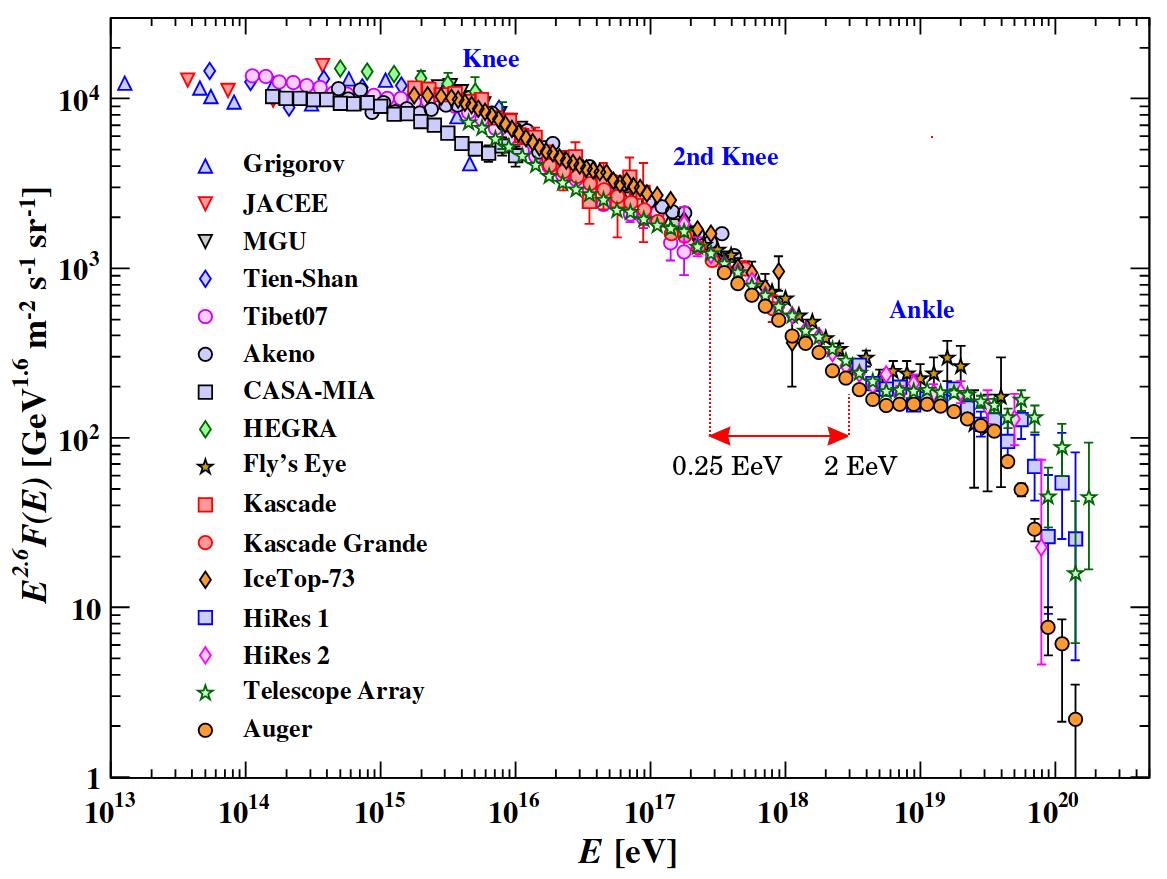
\includegraphics[width=\textwidth]{auger_spectrum_v2.png}
	\caption{Espectro de rayos cósmicos medidos mediante lluvias atmosféricas en función de la energía $E$. Figura extraída de \cite{PGD}}
	\label{fig:spectra}
\end{figure}
	

\section{Introducción}

Para realizar un estudio con mucha estadística de los CRs hasta altas energías se diseñó el Observatorio Pierre Auger. Las propiedades medidas de los lluvias extendidas determinan la energía y la dirección de arribo de cada CR, además de proveer información sobre la distribución de la composición del CR. El Observatorio Pierre Auger en la Provincia de Mendoza, Argentina ha registrado eventos desde el año 2004 mientras se agregaban detectores hasta su terminación en el 2008.

\section{Detección de Rayos Cósmicos}

Una característica esencial del Observatorio es la capacidad de observar lluvias atmosférica extendidas (EAS) simultáneamente mediante dos técnicas distintas, combinando los detectores de superficie (SD) y los detectores de fluorescencia (FD). Los SD son un conjunto de 1660  detectores Cherenkov con agua hiper-pura colocados en un arreglo triangular, con una distancia de $1.5\,$km cubriendo $\sim3000\,$km$^2$, además de un arreglo más pequeño llamado \emph{Infill} separados por $750\,$m. El arreglo principal son los detectores de superficie distanciados 1500\,m, que en el presente trabajo se  referencia como \emph{SD 1500\,m} se muestra en la Fig.\,\ref{fig:auger_sd}. Los FD están colocados en cuatro edificios alrededor del arreglo de SD: Coihueco, Loma Amarilla, Los Morados y Los Leones indicados en el mapa en la Fig.\,\ref{fig:auger_sd}. Cada edificio contiene 6 FD, donde cada uno tiene un campo de visión de $30^o\times30^o$, cubriendo así cada uno $180^o$ en la horizontal.

El área del observatorio es generalmente plana, la altitud de los detectores varía entre $1340\,$m y $1610\,$m, con una altitud media de $\sim1400\,$m. Estos detectores están distribuidos entre las latitudes $35.0^o$ S y $35.3^o$ S y entre las longitudes $69.0^o$ W y $69.4^o$ W.


\subsection{ El detector de superficie y el detector de Fluorescencia}

Un SD consiste en un tanque de polietileno de $3.6\,$m de diámetro que contiene $12\,000$ litros de agua agua hiper-pura. Su interior está recubierto por una lámina de alta reflectividad. En la parte superior se encuentran tres foto-multiplicadores (PMT) distribuidos simétricamente  a $1.2\,$m respecto al centro del tanque. Los mismos colectan la radiación Cherenkov producida por una partícula cargada relativista que pasa por el agua del detector. La altura del tanque de $1.2\,$m lo hace sensible a fotones de altas energías, que pueden convertirse en pares electrón-positrón en el volumen de agua \cite{como_funciona_auger}.

El detector de fluorescencia (FD) consiste en 24 telescopios de fluorescencia, esquematizados en la Fig\,\ref{fig:FD}, distribuidos en 4 distintos lugares en los límite del observatorio. %Estos 4 sitios son: Los Leones, Loma Amarilla, Los Morados y Coihueco, donde 6 de estos telescopios están instalados. 
Cada telescopio tiene un espejo esférico segmentado de 13$\,m^2$ y una cámara que consiste en 440 PMTs ordenados en una grilla de 22x20. Cada telescopio tiene un campo de visión de $30^o\times30^o$.%, por lo tanto cada edificio cubre $180^o$ en acimut.

\begin{figure}[H]
	\centering
	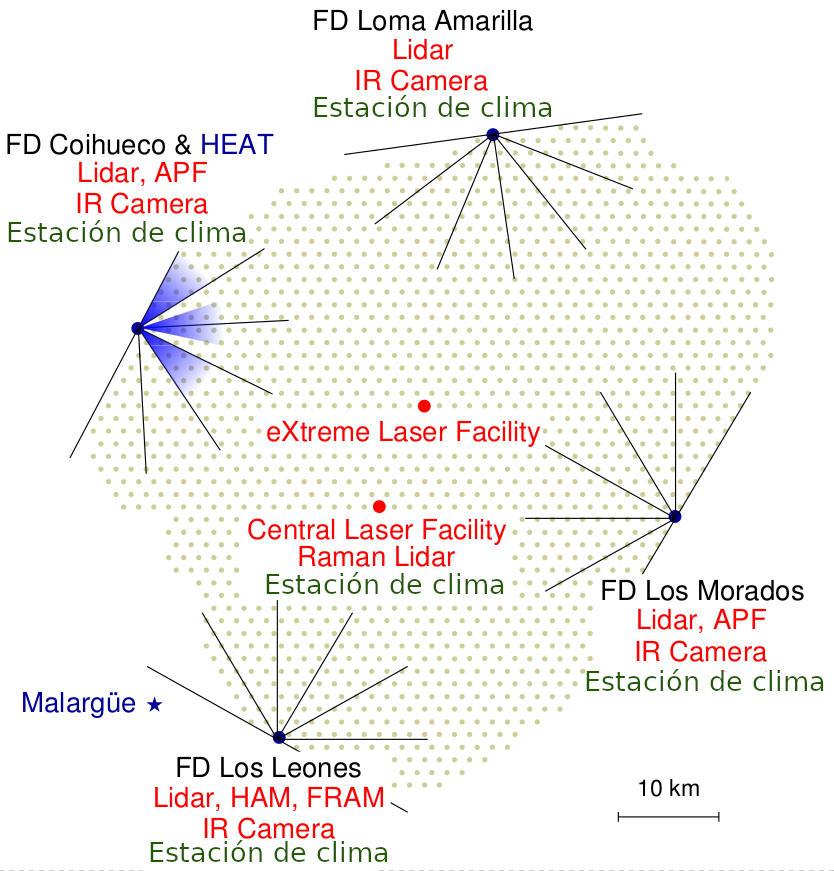
\includegraphics[width=0.75\textwidth]{auger_sd.png}
	\caption{Distribución de los tanques del SD en el área del Observatorio Pierre Auger. Se muestra la ubicación de las estaciones del clima, otros módulos instalados sobre el observatorio y la posición de los detectores de fluorescencia (FD). Figura extraída de \cite{como_funciona_auger}}
	\label{fig:auger_sd}
\end{figure}

\begin{figure}[H]
    \begin{subfigure}[t]{0.45\textwidth}
	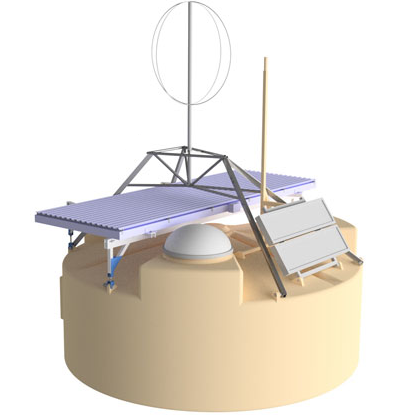
\includegraphics[width=\textwidth]{tanque.png}
	\caption{Detector de radiación Cherenkov con los elementos de la actualización para \emph{Auger Prime}} 	\label{fig:tanque}
    \end{subfigure}%
    \hspace{\fill}
    \begin{subfigure}[t]{0.5\textwidth}
	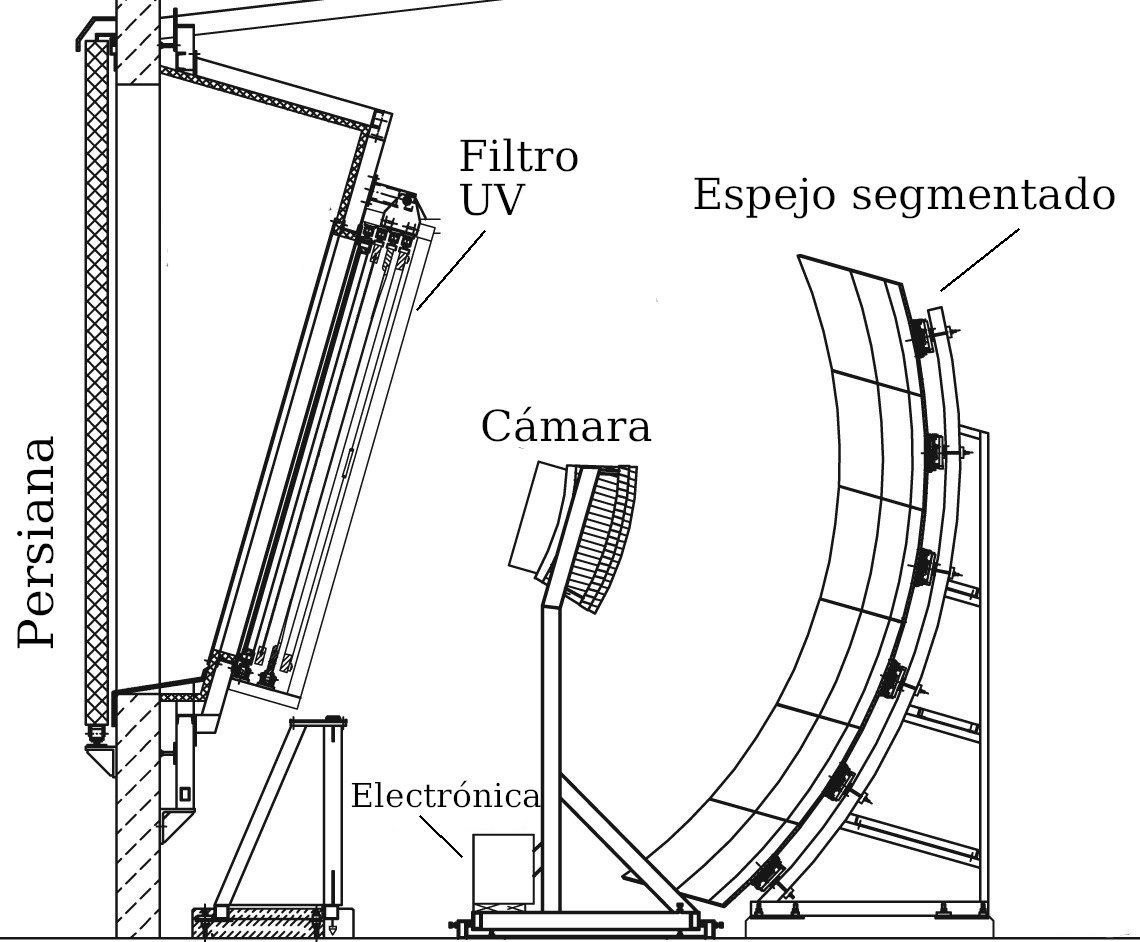
\includegraphics[width=\textwidth]{fd.png}
	\caption{Esquema simplificado de un telescopio de fluorescencia. Extraído de \cite{kit_oracle}}
	\label{fig:FD}
    \end{subfigure}%
    \caption{Detectores empleados por el Observatorio Pierre Auger para la detección de rayos cósmicos.}
	\end{figure}

El FD mide los fotones ultravioletas producidos por la componente electromagnética de la EAS. Mientras se produce la lluvia en la atmósfera, algunos átomos de nitrógeno se excitan y se desexcitan emitiendo fotones. El uso del FD para detectar estos fotones es solo posible en noches sin nubes y sin luna. La posible atenuación de los fotones en la atmósfera es tenida en cuenta para la estimación de energía. Ya que esta estimación se basa en la cantidad de fotones detectados. Otro factor a tener en cuenta es la presencia de aerosoles, como humo o polvo, esto se realiza midiendo la profundidad atmosférica óptica vertical \emph{Vertical Atmosferic Optical Depth (VAOD)}. Estas mediciones son realizadas por los láseres de las instalaciones de Central Laser Facility (CLF) y de eXtreme Laser Facility (XLF), cuyas ubicaciones se muestra en la Fig.\ref{fig:auger_sd}.

\subsection{Diseño híbrido}\label{seccion:sd_eff}

El SD detecta un corte de EAS que llega al nivel del suelo, los WCDs detectan la componentes electromagnética y muónica de la lluvia. Cabe resaltar que el SD funciona las 24 horas del día, por lo que detecta una mayor cantidad de eventos que el FD. Existen métodos para determinar la dirección de arribo y la energía del primario.  La exposición se calcula contando la cantidad de hexágonos activos en un tiempo dado, y multiplicado la apertura de una sola celda hexagonal que vale $4.59\,$km$^2$.sr para lluvias verticales. El SD tiene la propiedad de que la calidad de sus mediciones aumenta con la energía del EAS. La exposición instantánea del SD se calcula fácilmente, especialmente para energías mayores a 3 EeV, donde la EAS detectada por cualquier parte del SD es detectada con 100\% de eficiencia independientemente de la masa del primario que inicio la EAS.

El FD es usado para generar una imagen del desarrollo del EAS en la atmósfera. La luz de fluorescencia es emitida isotrópicamente en la parte ultravioleta del espectro, y es producida predominantemente por la componente electromagnética de la lluvia. Los períodos de observación están limitados a las noches sin luna y con buen clima, pero la ventaja del FD es la posibilidad de ver el desarrollo de la lluvia. Dado que la producción de la fotones por fotoluminiscencia es proporcional a la energía depositada en la atmósfera, se puede medir la energía del primario mediante calorimetría. Otro aspecto importante del FD es la posibilidad de medir la profundidad de la atmósfera donde la lluvia alcanza su máximo desarrollo, $X_{max}$, esta cantidad es uno de los más directos indicadores de la composición de masa. \cite{data}

\section{Reconstrucción de eventos de los detectores  de superficie}

\subsection{Selección de eventos}

La reconstrucción de la energía y la dirección de arribo de los CRs se realiza mediante las señales medidas por el SD. La dirección es reconstruida mediante  el tiempo de llegada de las señales registradas por estaciones individuales del SD. Para garantizar la selección de eventos bien contenidos en el SD, se aplica el corte llamado \emph{6T5}. Este corte considera solo a los eventos donde el tanque con mayor señal está rodeado por otros 6 tanques activos. Esta condición asegura una buena reconstrucción de la energía. Al mismo tiempo, este corte simplifica el cálculo de la exposición \cite{exposure}, importante  para el análisis del espectro. Para estudios de dirección de arribo pueden utilizar cortes menos estrictos.

\subsection{Reconstrucción de las lluvias}

En una primera aproximación para la dirección de arribo de la lluvia se obtiene ajustando los tiempos de llegada de la señal en cada tanque. Para eventos con suficientes tanques disparados, estos tiempos de llegada pueden ser descritas como la evolución un frente de lluvia como una esfera que crece con la velocidad de la luz. Los puntos de impacto del EAS con el suelo son obtenidas mediante ajustes a las señales de los tanques. Este ajuste se realiza con un función de distribución lateral (LDF). La LDF también tiene en cuenta la probabilidad de que los tanques no sean disparados y que los tanques con mayor señal estén saturados.

Un ejemplo de la señal que deja un evento sobre el SD 1500 m se muestra en la Fig.\,\ref{fig:evento_sd}. Este evento fue producido por un rayo cósmico de ($104\pm11$)\,EeV con un ángulo cenital de ($25.1\pm0.1 ^o$). La LDF de las señales para este evento se muestra en la Fig.\,\ref{fig:evento_S1000}. La función utilizada para el ajuste de la LDF es una función  $f_{LDF}$ propuesta por Nishimura-Kamata-Greisen \cite{data}
\begin{align*}
	%S(r) = S(r_{opt})\bigg(\frac{r}{r_{opt}}\bigg)^{\beta}\bigg(\frac{r+r_1}{r_{opt}+r_1}\bigg)^{\beta + \gamma}
	S(r) &= S(r_{opt})f_{LDF}(r)\\
	f_{LDF}(r)&=\bigg(\frac{r}{r_{opt}}\bigg)^{\beta}\bigg(\frac{r+r_1}{r_{opt}+r_1}\bigg)^{\beta + \gamma}
\end{align*}
donde $f_{LDF}$ está normalizado tal que $f_{LDF}(r_{opt})=1$ y $r_{opt}$ es la distancia óptima, %$r_1=700\,$m 
y $S(r_{opt})$ es usado para estimar la energía. Para el arreglo SD 1500\,m, el parámetro $r_{opt}=1000\,$m, por lo tanto el tamaño de la lluvia o \emph{shower size} es el valor de S(1000). Dado que la forma de la LDF es desconocida, la forma funcional propuesta para la función $f_{LDF}$ fue elegida empíricamente.  El parámetro $\beta$ depende del tamaño de la lluvia y del ángulo cenital. Los eventos verticales, es decir los eventos con $\theta < 60^o$, son medidas en una etapa menos desarrollada que eventos más inclinados. Los eventos con $\theta>60^o$ atraviesan un mayor cantidad de atmósfera.


\begin{figure}[H]
	\begin{small}
		\begin{center}
			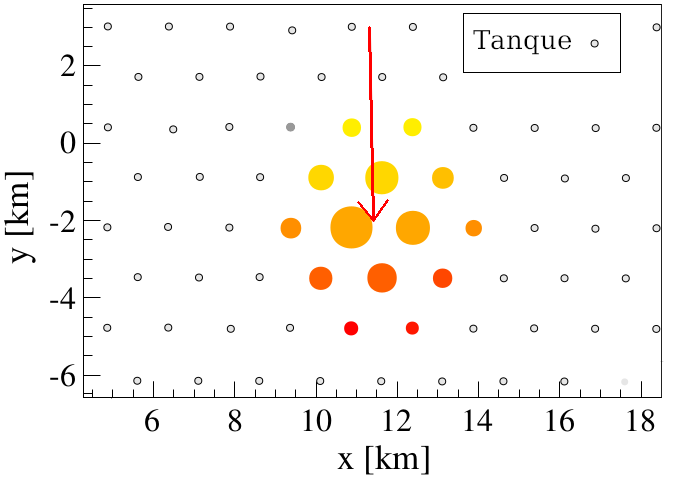
\includegraphics[width=0.65\textwidth]{evento_sd.png}
		\end{center}
		\caption{Ejemplo de la señal dejada por un evento de ($104\pm11$)\,EeV de energía con un ángulo cenital de ($25.1\pm0.1 ^o$) sobre el arreglo principal SD 1500 m. La flecha indica la dirección de arribo de la lluvia. Los colores de los círculo representa el tiempo de arribo de la lluvia, los primeros en amarillo y los últimos en rojo. En área de los círculo pintados es proporcional a logaritmo de la señal. Figura extraída de \cite{como_funciona_auger}. } 	\label{fig:evento_sd}
	\end{small}
\end{figure}


\begin{figure}[H]
	\begin{small}
		\begin{center}
			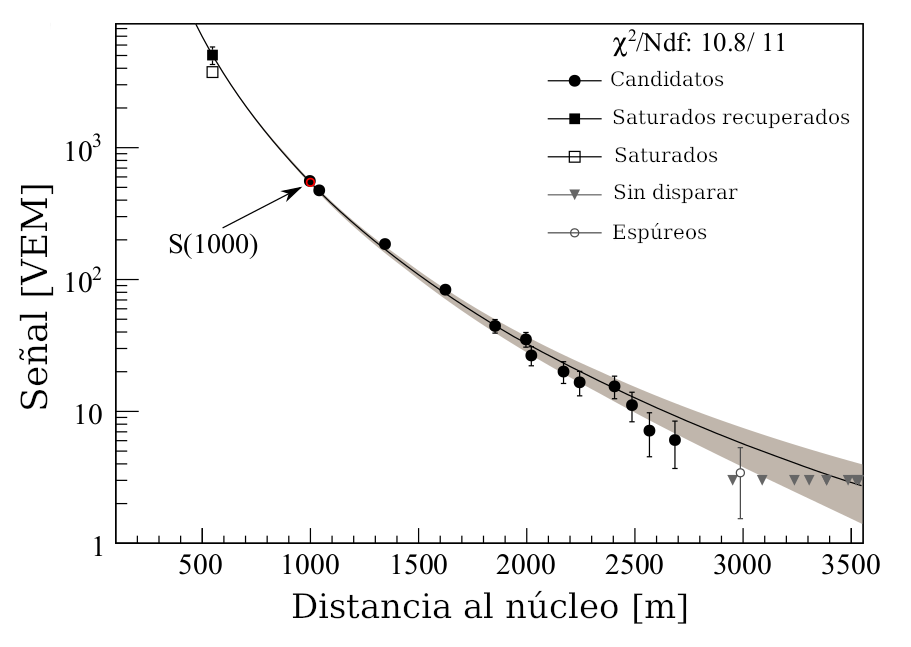
\includegraphics[width=0.65\textwidth]{evento_s1000.png}
		\end{center}
		\caption{Dependencia de la señal con la distancia del núcleo de la lluvia de un evento de ($104\pm11$)\,EeV de energía con un ángulo cenital de ($25.1\pm0.1 ^o$). La función ajustada es la función de distribución lateral (LDF). Del ajuste se obtiene el valor de S(1000). Figura extraída de \cite{como_funciona_auger}. } 	\label{fig:evento_S1000}
	\end{small}
\end{figure}


\subsection{Calibración de la energía}

Para una energía dada, el valor de S(1000) disminuye con $\theta$ debido a la atenuación de las partículas de la lluvia. Asumiendo un flujo isotrópico de los CR primarios sobre la parte superior de la atmósfera, se obtiene la atenuación de los datos mostrados en la Fig.\,\ref{fig:s1000_theta}  usando el método de Corte de Intensidad Constante (CIC) \cite{CIC}. La curva de atenuación $f_{CIC}(\theta)$ fue ajustado con un polinomio de orden 3 del tipo $f_{CIC}(\theta)=1+ax+bx^2+cx^3$, donde $x=\cos^2(\theta) - \cos^2(38^o)$. Según lo presentado por la colaboración \cite{collaboration2013pierre}, los valores son $a=0.980\pm0.004$, $b=-1.68\pm0.01$ y $c=-1.30\pm 0.45$, aunque estos coeficientes cambian ligeramente con la energía \cite{data}. El ángulo cenital $\theta=38^o$ se toma como un punto de referencia para convertir S(1000) a S$_{38}$ mediante $S_{38}=S(1000)/f_{CIC}(\theta)$. Este valor S$_{38}$ puede considerarse como la señal S(1000) que hubiera tenido un evento que fue detectado mediante el SD con $\theta=38^o$.

Los eventos con $\theta<60^o$  que fueron detectados por el SD y por el FD son utilizados para relacionar el tamaño de la lluvia con la energía  E$_{FD}$ medida por calorimetría por el FD.  La correlación entre S$_{38}$ y E$_{FD}$ se calcula mediante el método de máxima verosimilitud, que considera la evolución de las incertezas con la energía. La relación entre S$_{38}$ y $E_{FD}$ se describe mediante un función de potencia como se muestra en la Ec.\,\ref{eq:s38_energy}
\begin{equation}
	E_{FD}= A\, (S_{38}/VEM)^B
	\label{eq:s38_energy}
\end{equation}
donde los parámetros obtenidos son $A=(1.86\pm0.03)\times 10^{17}\,$eV y $B=(1.031\pm0.004)$  \cite{tobepublished}. En la Fig.\,\ref{fig:efd_s38} se observa el ajuste y la relación entre  S$_{38}$ y E$_{FD}$


\begin{figure}[H]
    \begin{subfigure}[t]{0.51\textwidth}
	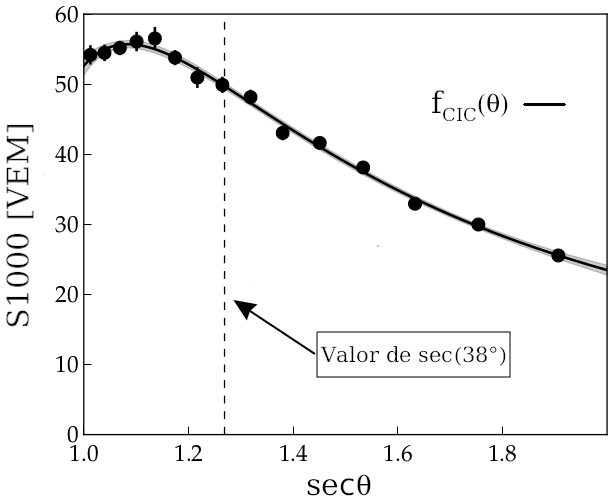
\includegraphics[width=\textwidth]{s1000_theta.png}
	\caption{Curva de atenuación descrita por un polinomio de orden 3. En este ejemplo se deducen los coeficientes de la dependencia del S(1000) a S$_{38}\approx 50\,$VEM que corresponde a un energía de $10.5\,$EeV.} 	\label{fig:s1000_theta}
    \end{subfigure}%
    \hspace{\fill}
    \begin{subfigure}[t]{0.45\textwidth}
	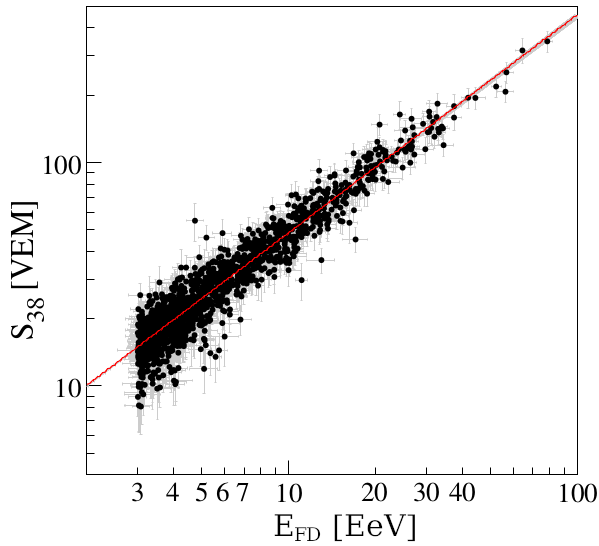
\includegraphics[width=\textwidth]{efd_s38.png}
	\caption{Correlación entre el valor S$_{38}$ y la energía $E_{FD}$ medida por el FD.} 	\label{fig:efd_s38}
    \end{subfigure}%
    \caption{Distintas calibraciones hechas para los eventos reconstruidos en el Observatorio Pierre Auger.}
	\end{figure}



\subsection{Monitoreo del clima}\label{seccion:clima}

Las condiciones atmosféricas, como la temperatura, presión y humedad, se deben tener en cuenta para estudiar el desarrollo de los EAS, así como también para estudiar la cantidad de fotones de las lluvias sobre los moléculas de N$_2$, emitidos por fluorescencia. Distintas estaciones monitorean las condiciones atmosféricas sobre el Observatorio Pierre Auger, cuatro cerca  de los edificios donde se encuentran los FD y uno cerca del centro del SD 1500\,m. Para este trabajo se utilizaron las mediciones de la presión y temperatura registradas la mayor parte del tiempo en la estación del clima cerca del CLF, la misma realiza una medición cada intervalo de 5 minutos la mayor parte del tiempo. Cuando no se cuenta con datos registrados para intervalos entre 10 minutos hasta 3 horas, en estos casos se utiliza una interpolación de los datos medidos. Si el período de tiempo es mayor a 3 horas, los eventos durante este periodo no son considerados para la determinación de los efectos del clima en la señal detectada por el SD 1500\,m.

\chapter{Análisis de los efectos del clima sobre los datos del Observatorio Pierre Auger}
	
Para el análisis y ajuste se trabajaó con dos conjuntos de datos distintos. El primero fue el conjunto de datos que la colaboración Pierre Auger presentó en la Conferencia Internacional de Rayos Cósmicos (ICRC) del año 2015, este conjunto de datos se utilizó para el cálculo de las correcciones climáticas al estimador de energía \cite{aab2017impact}. El segundo conjunto de datos se presentó en la ICRC del año 2019. Entre estos dos conjuntos de datos existieron cambios en la reconstrucción de energía de los eventos, en particular en el valor de la señal de S$(1000)$ \cite{isabel}, además de agregar la corrección por las modulaciones del clima propuesto en \cite{aab2017impact} sobre este mismo valor de señal y se implementó una función de corte de intesidad constante CIC que varía en función de la energía. El objetivo de este capítulo es comprobar si la corrección del clima de la reconstrucción de eventos es adecuada.

\section{La física detrás de la modulación del clima}\label{seccion:fisica_clima}

El SD mide las 24 horas del día las lluvias de partículas que llegan al suelo. Las señales registradas por los WCDs, ya sea mediante la componente electromagnética o muónica de las EAS, se usan para determinan la posición del núcleo, la dirección de arribo del CR y la energía del primario. La señal de los eventos son ajustados mediante un función de distribución lateral (LDF) para obtener una señal de referencia $S(1000)$. Existieron cambios en los parámetros de la LDF y, por lo tanto, de valor de $S_{38}$, utilizado para estimar la energía del primario. La conversión de $S(1000)$ a $S_{38}$ se realiza mediante el método de corte de intensidad constante (CIC) explicado anteriormente. Además en la nueva reconstrucción el CIC es función de la energía.

\subsection{Trabajos anteriores}

Debido a la modulación del clima dependiente de la estaciones, es de esperarse encontrar una modulación diaria y anual sobre la cantidad de eventos observados por el SD. Ya que en días con menor densidad y presión atmosférica, los tanques detectan eventos por debajo del umbral con mayor facilidad. Este fenómeno fue estudiado por trabajos anteriores realizados por la colaboración Pierre Auger \cite{aab2017impact} \cite{collaboration2009atmospheric}. En particular, el trabajo \cite{aab2017impact} consideró el retraso que tienen los cambios de  la temperatura a distintas alturas sobre la superficie, como se muestra en la Fig\,\ref{fig:delay} que son datos del GDAS (Global Data Assimilation System) promediados por hora del día. Posteriormente esta corrección fue implementada en el proceso  de análisis de datos del observatorio.


En la Fig.\,\ref{fig:delay} se observa que los ajustes realizados a las variaciones de la temperatura  según la hora del día con una función del tipo $T(t) = T_{media} + A\times \sin((t-t_d)\nicefrac{\pi}{12\,\text{hs}})$.  En la Tabla\,\ref{tabla:delay} se observa que entre 1400\,m (altitud del observatorio Pierre Auger) y la mayor altitud medida por el GDAS existe un corrimiento de $2.1\pm0.7\,$hs.

Como la relación entre la densidad y la temperatura del aire están relacionadas mediante la expresión $\rho \approx \nicefrac{0.3484P}{T +273.16}\,$kgm$^{-3}$, con P en hPa y T en  $^o$C \cite{aab2017impact}, el corrimiento de la temperatura al aumentar la altitud también se ve reflejada en la densidad. Como la misma es una variable importante para el desarrollo de la cascada en al atmósfera, este retraso debe tenerse en cuenta.

\begin{figure}[H]
	\centering
	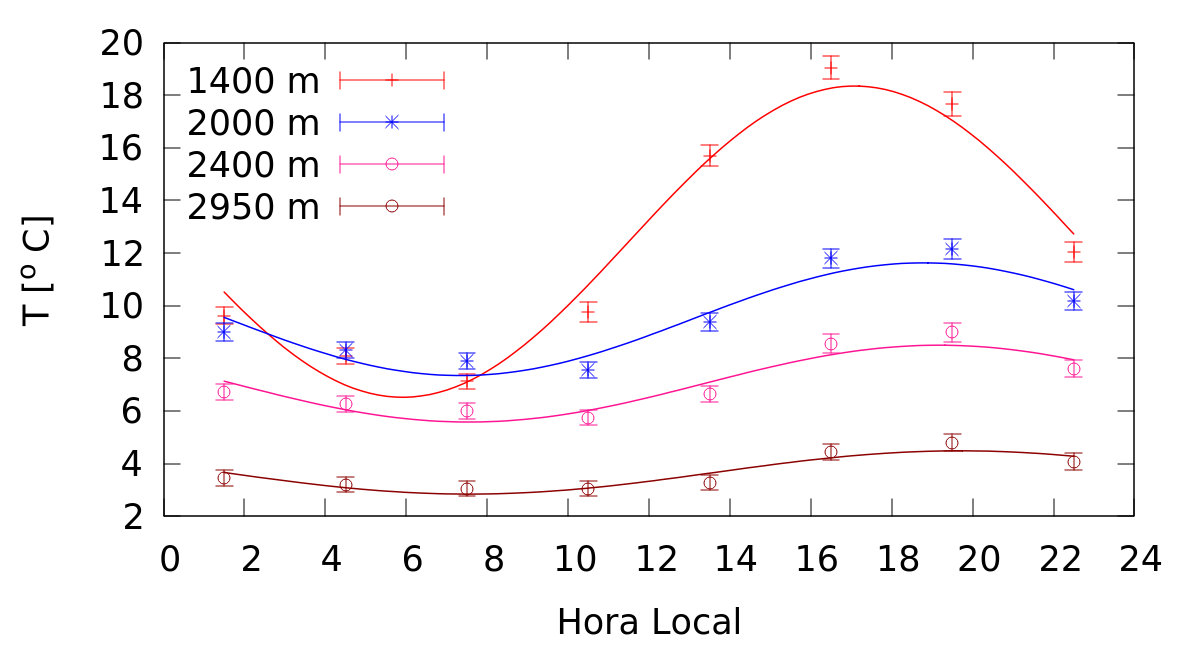
\includegraphics[width=0.65\textwidth]{delay.png}
	\caption{Mediciones de la temperatura a distintas alturas sobre el nivel del mar en función de la hora del día en Malargüe. (Hora Local: UTC-3).}
	\label{fig:delay}
\end{figure}
\begin{table}[H]
\centering
\begin{tabular}{|c|c|c|c|}
\hline
Altura\,[m] & 	T$_{media}$\,[$^o$\,C] 	& A [$^o$\,C] 	& t$_d$ [h] 	\\ \hline
1400		& 	$12.4\pm0.5$			& $5.6\pm0.6$ 	& $12.5\pm0.5$ 		\\ \hline
2000		& 	$9.5\pm0.2$				& $2.1\pm0.3$ 	& $10.8\pm0.6$ 		\\ \hline
2400		&  	$7.0\pm0.2$				& $1.4\pm0.2$	& $10.7\pm0.6$ 		\\ \hline
2950		& 	$3.7\pm0.1$				& $0.8\pm0.1$	& $10.4\pm0.6$ 		\\ \hline
\end{tabular}
\caption{Características de la modulación de la temperatura en función de la altura sobre el nivel del mar.}\label{tabla:delay}
\end{table}

\subsubsection{Efectos de la atmósfera sobre los rayos cósmicos}

La variación de las condiciones atmosféricas afecta las señales de las lluvias atmosféricas extendidas. Estas señales pueden ser detectadas en la superficie por un arreglo de detectores, como los que se encuentran en el Observatorio Pierre Auger. Estos efectos pueden inducir errores sistemáticos en la reconstrucción de energía de los rayos cósmicos. Se han realizado  trabajos anteriores sobre los efectos del clima sobre la señal detectada en el Observatorio Pierre Auger \cite{collaboration2009atmospheric} \cite{aab2017impact}. En este trabajo se estudió eventos con energía mayor a $1\,$EeV entre los años 2005-2018, extendiendo los periodos de tiempo estudiados anteriormente.
%444444444444444444444444444

Para entender los parámetros utilizados para describir a la lluvia, debemos entender que son la longitud de radiación $X_0$, la profundidad de la lluvia $X_{max}$ y el radio de Molière $r_M$. La longitud de radiación definida como $X_0=\nicefrac{d}{2}$,  donde $d$ es un parámetro que indica cuanta cantidad de materia debe atravesar un partícula cargada relativista para perder un factor de $\approx 50\%$ de su  energía. El $X_0$ depende del material que atraviesa la partícula, y tiene unidades de [g\,cm$^{-2}$]. La profundidad de la lluvia $X_{max}$ de una cascada puramente electromagnética, i.e. iniciada por un fotón, tiene la siguiente expresión \cite{matthews2005heitler}
\begin{equation}
 	X_{max} = X_0{ln(\frac{E}{\xi^e_c})}
 \end{equation} 
donde  $\xi^e_c$ es la energía crítica para la cual las pérdida de energía por radiación supera a la pérdidad de energía por colisión, en el aire $\xi^e_c=85\,$MeV. Por último, el radio de Molière $r_M$ que puede expresarse como 
\begin{equation}
	r_M= \frac{E_s}{\xi^e_c}\frac{X_0}{\rho}
\end{equation}
es la máxima profundidad transversal que alcanza la lluvia. El valor de $E_s\approx21\,$MeV caracteriza las pérdidas por dispersión. Usualmente un cilindro con un radio $r_M$ contiene al 90\% de la energía depositada en la atmósfera por el primario. El radio de Molière local en el aire para una altura $h$ puede definirse como $r_M = \nicefrac{9.6\,\text{gcm}^{-2}}{\rho(h)}$ \cite{gora2006universal}. 
%444444444444444444444444444

Las variables atmosféricas importantes que afectan al desarrollo de la EAS en la atmósfera son la presión y la densidad del aire. Por un lado la presión es una medida de cantidad de materia que atraviesa el CR. Si la presión sobre la superficie aumenta implica que la lluvia va a atravesar más partículas, y por el contrario si la presión disminuye la lluvia tiene menos materia para interactuar. Esto afecta el desarrollo longitudinal de la lluvia cuando llega a la superficie. En la Fig.\,\ref{fig:eas} se muestran una esquema simplificado de las interacciones en al atmósfera de un primario de la misma energía. En la figura de la izquierda representa la lluvia donde la presión y la densidad está por encima de la media, y la figura de la derecha representa un lluvia donde la presión y la densidad de la atmósfera están por debajo de la media.

\begin{figure}[H]
	\centering
	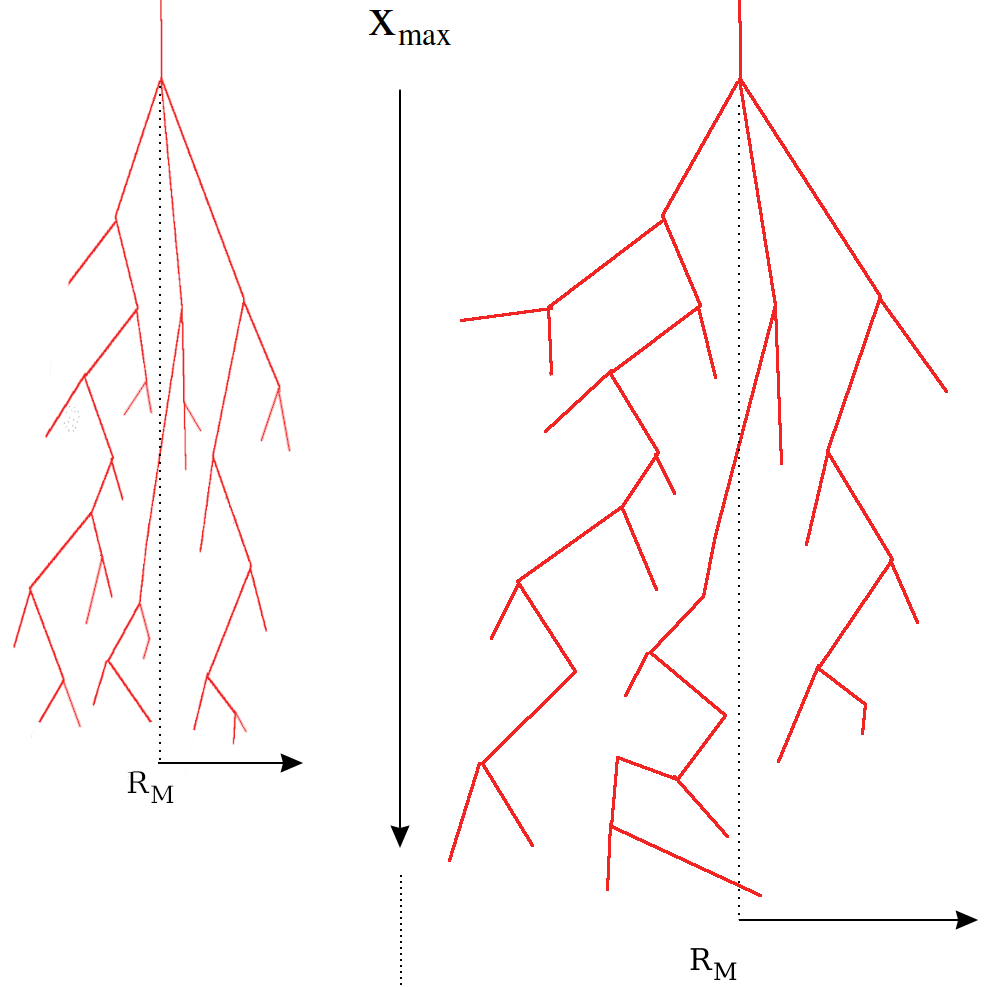
\includegraphics[width=0.5\textwidth]{eas.png}
	\caption{Diagramas simplificado de un lluvia de la misma energía para distintas condiciones atmosféricas}
	\label{fig:eas}
\end{figure}

Estos efectos se ven reflejados en la señal sobre el SD del Observatorio Pierre Auger. La extensión de la señal sobre el SD, es decir el $r_M$ puede cambiar según la densidad de la atmósfera por encima del SD. Los valores de $r_M$ relevantes para la señal medida son a nivel del suelo y a 1000 m. Esto implica que las variaciones de densidad (o de temperatura) a estas alturas están relacionadas con las variaciones al nivel del suelo. La variación a $\sim2400\,$m sobre el nivel del mar está atrasada dos horas con respecto a la variación sobre el Observatorio, que se encuentra a $\sim1400\,$m sobre el nivel del mar. Otro aspecto importante es que la amplitud de está variación disminuye con la altura. Entre las dos altitudes mencionadas existen una relación de aproximadamente $\nicefrac{1}{3}$ entre las amplitudes. 

\subsubsection{Modelo teórico}

Considerando lo analizado en \cite{aab2017impact} \cite{collaboration2009atmospheric}, en este trabajo se propone la siguiente modulación, presentada en la Ec.\,\ref{eq:signal}, para la señal S que reciben los tanques 
\begin{equation}
	S=S_0\big(1+\alpha_P(P-P_0) +\alpha_{\rho}(\rho_{media}-\rho_0) + \beta_{\rho}(\rho_{2h}-\rho_{media})\big)
	\label{eq:signal}
\end{equation}
donde $S_0$ es la señal  del evento en condiciones atmosféricas medias, $P$ es la presión en el momento del evento, $P_0=862\,$hPa es la presión media en el rango de tiempo estudiado, $\rho_{media}$ es la densidad  media del aire en 24\,hs, $\rho_0=1.06\,$kgm$^{-3}$ es la densidad media durante el periodo estudiado, $\rho_{2h}$ es la densidad que se midió dos horas antes del evento  y los coeficientes $\alpha$ y $\beta$ tiene en cuenta la modulación del clima sobre la señal.  Si consideramos la tasa $R_{ang}$  por ángulo sólido $\Omega$

\begin{equation}
	\frac{dR_{ang}}{d\Omega} = \int_{S_{min}}^{\infty} P_{Tr}(S,\theta) d\Phi_{CR}
	\label{eq:rate_angular}
\end{equation}
donde $P_{Tr}$ es la probabilidad de que sea detectado un evento para un valor de señal mínimo $S_{min}$ dado, y $\Phi_{CR}$ es la densidad de eventos por ángulo sólido. La función $P_{Tr}$ tiene en cuenta la eficiencia del disparo de los tanques en función de la energía. Por ejemplo, para el SD 1500 m, como se mencionó anteriormente, la eficiencia máxima de disparo es a partir  de $3\,$EeV. Considerando  las Ecs.\,\ref{eq:s38_energy} y \ref{eq:expresion1} , se puede reescribir la Ec.\ref{eq:rate_angular} como integral de la señal medida S. Teniendo en cuenta que la corrección del clima es pequeña podemos escribir la Ec.\,\ref{eq:signal} como $S=S_0(1+\epsilon)$ y las Ecs. \ref{eq:expresion1} y \ref{eq:s38_energy}.
\begin{align*}
\frac{d\Phi_{CR}}{dE} 	&\propto E^{-\gamma} 					\qquad\qquad\qquad\qquad\qquad \quad \qquad \qquad		\frac{dE}{dS}  			= \frac{dE}{dS_0}\,\frac{dS_0}{dS}\\ 
					  	&= S^{-B\gamma}(1+\epsilon)^{B\gamma}    \qquad\qquad \qquad\qquad\qquad \qquad 				  	 = AB\,S^{B-1}\, (1+\epsilon)^{-B}\\
   		    			\frac{dR_{ang}}{d\Omega} &= \int_{S_{min}}^{\infty} P_{Tr}(S,\theta) \frac{d\Phi_{CR}}{dE} \frac{dE}{dS} dS\\
    						 &\propto \int_{S_{min}}^{\infty} P_{Tr}(S,\theta) \bigg( S^{-B\gamma}(1+\epsilon)^{B\gamma}\bigg) \bigg( AB\,S^{B-1}\, (1+\epsilon)^{-B}\bigg)dS\\
    						 &\propto A\,B (1+\epsilon)^{B\gamma - B}\int_{S_{min}}^{\infty} P_{Tr}(S,\theta) S^{-B\gamma +B -1} dS\\
\end{align*}

Dado que $\epsilon\,\ll\,1$, uno puede expandir la expresión $(1+\epsilon)^{B\gamma}$ hasta primer orden 
\begin{equation*}
	(1+\epsilon)^{B\gamma-B} \approx 1 + B(\gamma-1)\epsilon
\end{equation*}

Por lo que la expresión final queda de la siguiente forma

\begin{equation*}
	\frac{dR_{ang}}{d\Omega} \propto AB(1+B(\gamma - 1)\epsilon)\int_{S_{min}}^{\infty} P_{Tr}(S,\theta) S^{-B\gamma +B -1} dS
\end{equation*}

Considerando que $d\Omega= sin(\theta)d\theta d\phi$ y que el área efectiva  que tiene el observatorio para dado un evento con ángulo cenital $\theta$ es $M_{eff}=M\times cos(\theta)$, donde $M$ es el área activa del observatorio en el momento del evento. Podemos redefinir la tasa por área $R$ como

\begin{align*}
	dR 	&\propto \frac{dR_{ang}}{d\Omega} \frac{M_{eff}}{M} d\Omega \\
		&\propto \frac{dR_{ang}}{d\Omega}\, cos(\theta)\, sin(\theta)\,d\theta d\phi\\
		%&=  AB(1+B(\gamma - 1)\epsilon)\, cos(\theta)\, sin(\theta)\,d\theta d\phi \int_{S_{min}}^{\infty} P_{Tr}(S,\theta) S^{-B\gamma +B -1} dS\\
		&\propto  AB(1+B(\gamma - 1)\epsilon)\,dsin^2\theta d\phi\,\int_{S_{min}}^{\infty} P_{Tr}(S,\theta) S^{-B\gamma +B -1} dS
\end{align*}

Así pudiendo definir la tasa por área por $sin^2(\theta)$, independiente del valor de $\phi$

\begin{align*}
	\frac{dR}{d(sin^2\theta)} &\propto AB(1+B(\gamma-1)\epsilon)\, 2\pi \,\int_{S_{min}}^{\infty} P_{Tr}(S,\theta) S^{-B\gamma +B -1} dS
\end{align*}

Los parámetros $\alpha_P$, $\alpha_{\rho}$ y $\beta_{\rho}$ podrían depender del ángulo cenital o de la energía (por ende de S). En este trabajo se considera solamente la dependencia en $\theta$. Si $P_{Tr}$ es independiente de $\theta$, podemos absorber estas constantes y dejar la expresión como

\begin{equation}
	\frac{dR}{d(sin^2\theta)} = R_0\bigg[1+a_P(P-P_0) +a_{\rho}(\rho_{media}-\rho_0) + b_{\rho}(\rho_{2h}-\rho_{media})\bigg] 
	\label{eq:rate_sin2}
\end{equation}
donde los parámetros $a_P=B(\gamma-1)\alpha_{P}$, $a_{\rho}=B(\gamma-1)\alpha_{\rho}$ y $b_{\rho}=B(\gamma-1)\beta_{\rho}$, donde los parámetros B y $\gamma$ son conocidos.

\subsubsection{Estimador del ajuste}

Para determinar los parámetros del clima, se calcula la tasa de eventos por hora durante un periodo seleccionado normalizada con el área correspondiente a ese momento. Durante el trabajo se menciona la tasa de eventos, pero debe tenerse en cuenta que es la tasa normalizada con el área. Esta área es calculada a partir de la cantidad de hexágonos activos. Por lo tanto, una vez obtenida la tasa, se ajusta la misma mediante la expresión de la Ec.\ref{eq:rate_sin2}, obteniéndose los parámetros del clima.

Para realizar este ajuste, se supone que el número de eventos observado en una hora sigue una distribución de Poisson. Se realiza un ajuste de máxima verosimilitud (\emph{Maximum Likelihood Estimator}) para estimar los coeficientes del clima de la Ec.\ref{eq:rate_sin2}. La función a minimizar tiene la siguiente expresión 
\begin{equation}
	L=\prod_i\frac{\mu_i^{n_i} e^{-\mu_i}}{n_i!}
\end{equation}
donde $\mu_i$ es la media de la distribución de Poisson, que es el número de eventos esperado durante una hora que puede calcularse como
\begin{equation}
	\mu_i = R_0A_iC_i
\end{equation}
donde $R_0$ es la tasa promedio que se observaría si los parámetros atmosféricos fueran los de referencia, es decir $R_0=\nicefrac{\sum n_i}{\sum A_iC_i}$, donde $A_i$ es el área efectiva en el intervalo de tiempo $i$ y el parámetro $C_i$ tiene la forma

\begin{equation}
	C_i = 1+a_P(P-P_0) +a_{\rho}(\rho_{media}-\rho_0) + b_{\rho}(\rho_{2h}-\rho_{media}) 
\end{equation}
con $\rho_{2h}$, como fue mencionado anteriormente, es la densidad medida dos horas antes del evento.

\subsection{Condiciones climáticas y área activa del observatorio Pierre Auger}

Existen tres estaciones meteorológicas dentro del observatorio, que miden cada 5 minutos las condiciones climáticas en distintos puntos. Las ubicaciones de estas estaciones están indicadas en la Fig.\,\ref{fig:auger_sd}. La Fig.\,\ref{fig:clima_p_rho} se muestran las variaciones de los valores de presión y densidad en el periodo del $2005-2018$ con respecto a la media en este mismo periodo. En las mismas se observa las modulación anual de la densidad, Fig.\,\ref{fig:densidad_hora}, y al modulación diaria de la densidad, Fig.\,\ref{fig:area_auger}, que afecta a la detección de las lluvias por parte del SD. 

\begin{figure}[H]
        \begin{subfigure}[b]{0.49\textwidth}
        	\centering
			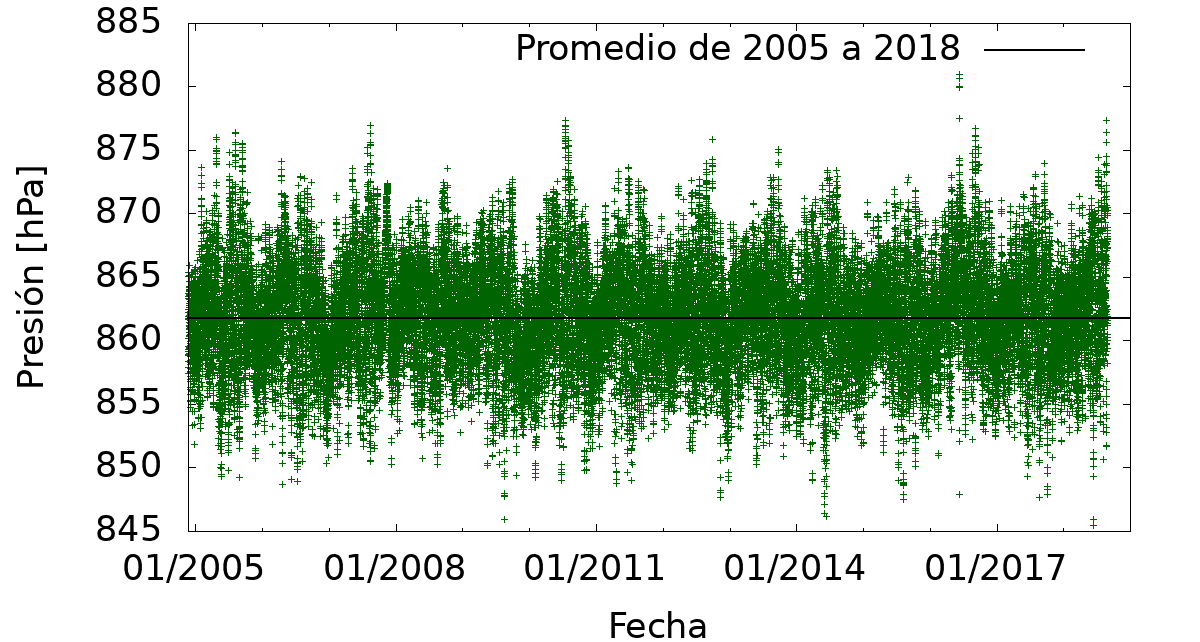
\includegraphics[width=\textwidth]{Graphs/clima/presion.png}
			\caption{Presión}
			\label{fig:presion}
		\end{subfigure}%
		\hspace{\fill}
        \begin{subfigure}[b]{0.49\textwidth}
			\centering	
			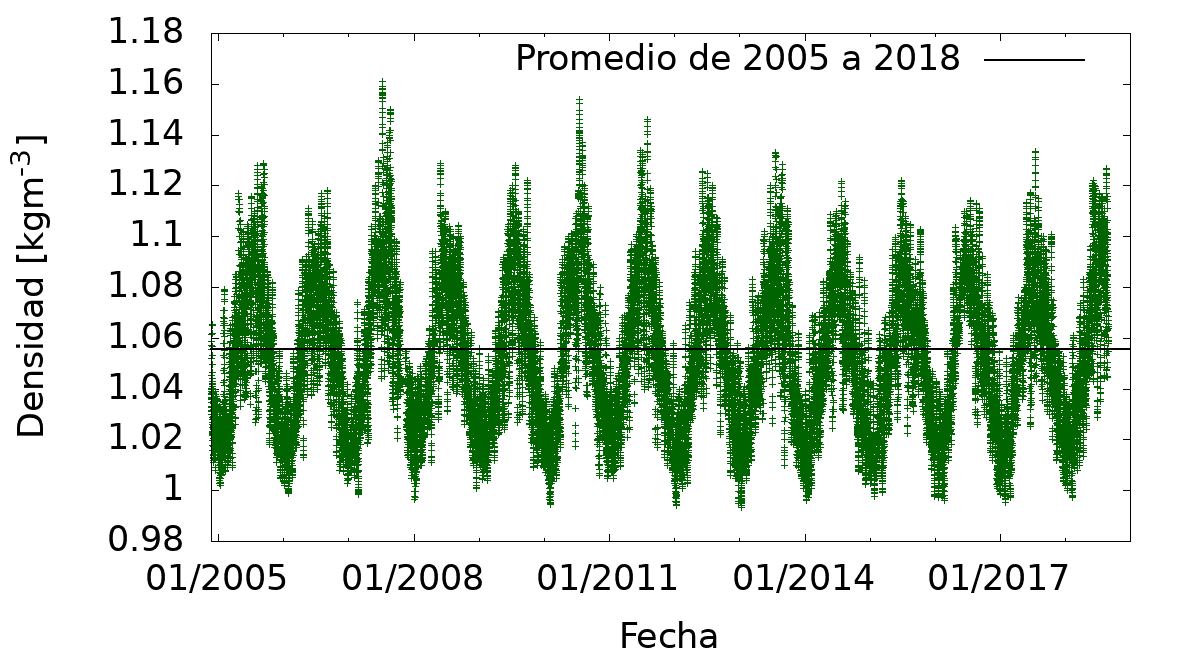
\includegraphics[width=\textwidth]{Graphs/clima/densidad_diaria.png}
			\caption{Densidad diaria}
			\label{fig:densidad_diaria}
        \end{subfigure}%
        \hspace{\fill}
        \begin{subfigure}[b]{0.49\textwidth}
        	\centering
			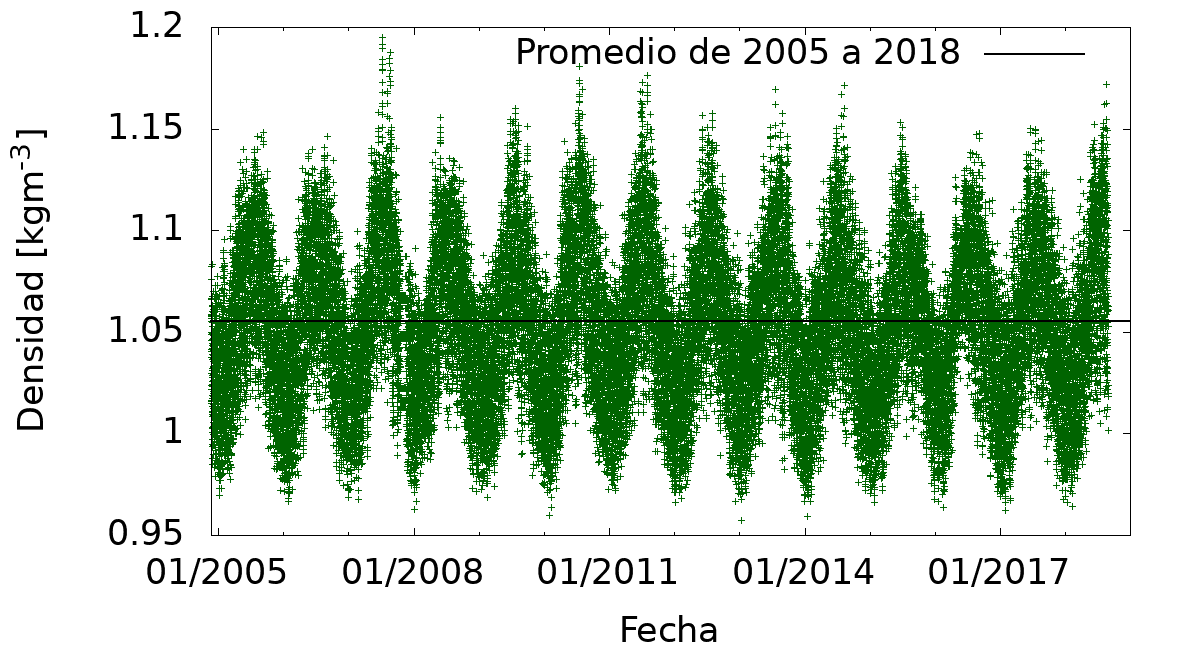
\includegraphics[width=\textwidth]{Graphs/clima/densidad_media_diaria.png}
			\caption{Densidad media por hora}
			\label{fig:densidad_hora}
		\end{subfigure}%
		\hspace{\fill}
        \begin{subfigure}[b]{0.49\textwidth}
			\centering	
			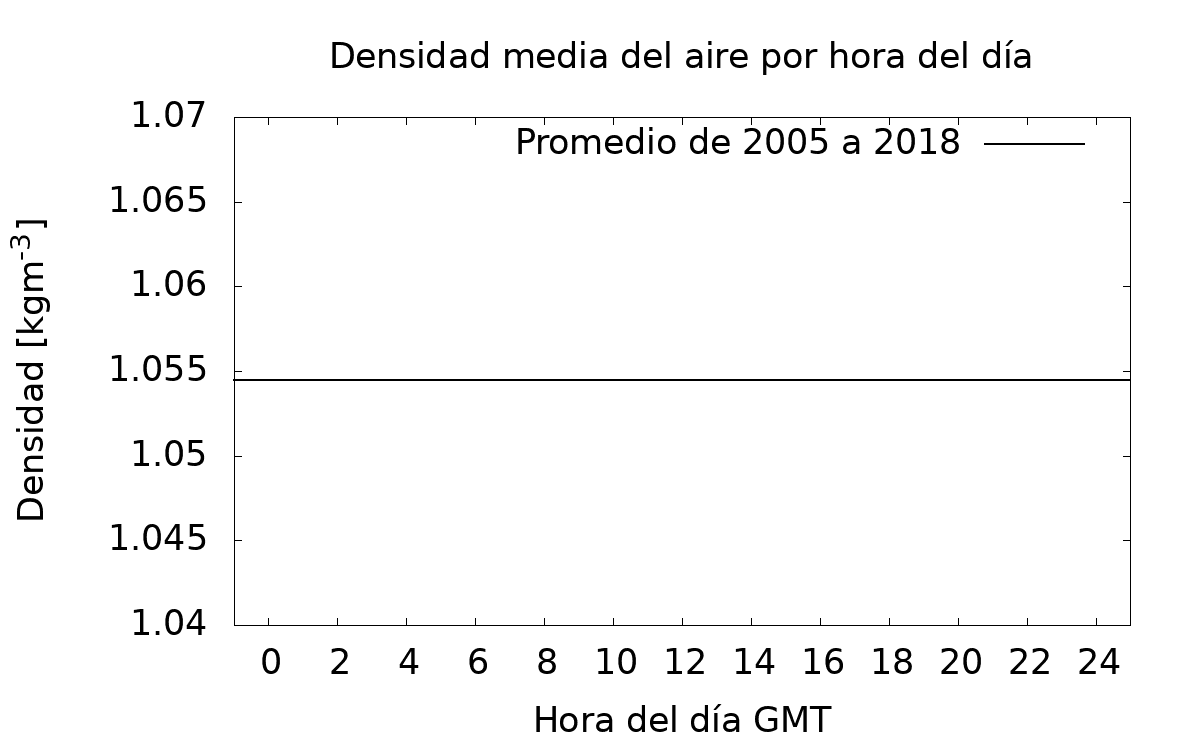
\includegraphics[width=\textwidth]{Graphs/clima/densidad_hod.png}
			\caption{Densidad media por hora del día.}
			\label{fig:area_auger}
        \end{subfigure}%
  \caption{Variaciones de las variables del clima en función del tiempo}
  \label{fig:clima_p_rho}
\end{figure}

	%|SD 1500
	\section{Resultados para el arreglo de detectores de superficie de 1500\,m de distancia}

	Para el SD 1500\,m se trabajó con los conjuntos de datos  presentados en la ICRC 2015  y  en la ICRC 2019.La señal de $S(1000)$ fue corregida en la reconstrucción oficial de eventos por la modulación del clima, por los parámetros obtenidos en \cite{aab2017impact}, mediante un análisis de los datos registrados  entre los años 2005-2015. En este trabajo se emula el análisis de datos realizado en \cite{aab2017impact} con los mismos datos, con el fin de verificar que se obtienen los mismos resultados. Luego se realizó un análisis similar con los datos de nueva reconstrucción de la señal $S_{38}$ sin la corrección del clima  del conjunto de datos de la ICRC 2019 en el periodo 2005-2018. %Posterior este análisis, se realizó un reconstrucción de la energía mediante un valor de $S_{38}$ del los datos de la ICRC 2019.% y la señal S$_{38}$ corregida por el clima S$_{38}$$_w$, para comparar resultados entre sí.

	Los coeficientes atmosféricos se obtienen tomando una energía mayor a $1\,$EeV en el caso de los datos de la ICRC 2015. Para el caso del análisis con el valor de $S_{38}$ de la ICRC 2019, se realiza el corte de eventos con el valor de $S_{38}$  que tiene un evento de $1\,$EeV. Es posible que estos coeficientes dependan de la energía, por ejemplo por la dependencia del logaritmo de la energía de $X_{max}$ o por los cambios de composición a distintas energías. En todo caso, se espera que estas dependencias sean pequeñas.% entonces los parámetros obtenidos deben describir  estos efectos. 

	Para asegurarse eventos con una buena reconstrucción de  energía, posición del núcleo y dirección de arribo, solo los eventos que están contenidos dentro del arreglo del SD son considerados. Este criterio requiere que el detector con mayor señal esté rodeado de 6 tanques activos. Teniendo en cuenta la geometría de arreglo de WCDs, se calcula el área efectiva mediante la suma del área asociada a cada tanque. El mismo contribuye un área de $\sqrt{3} \frac{d^2}{2}$, donde $d$ es la distancia entre WCDs en una grilla triangular. Como la cantidad de hexágonos activos varía con el tiempo también lo hace  el área efectiva del observatorio. En la Fig.\,\ref{fig:area} se muestra la evolución del área efectiva del SD 1500 m hasta el año 2018. La línea horizontal  limita el área mínima considerada para el análisis. Estos periodos de baja exposición no proveen información suficiente para caracterizar la modulación.
	Este valor de corte en el área corresponde aproximadamente al $10\%$ del valor nominal.
	\begin{figure}[H]
		\centering
		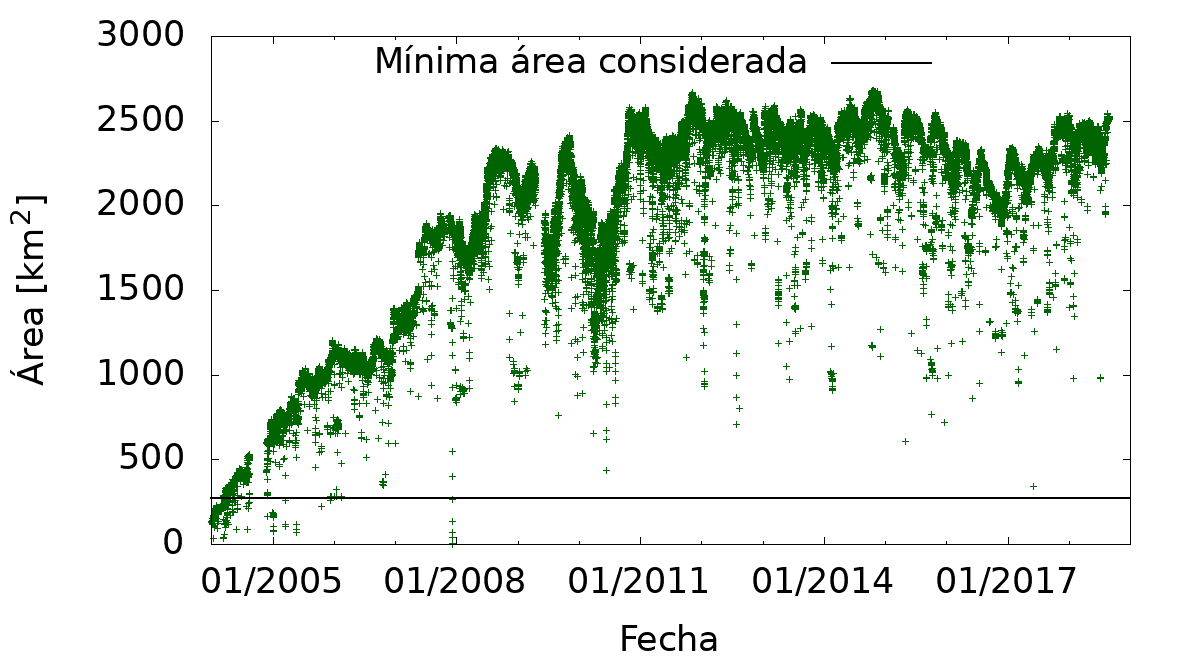
\includegraphics[width=0.5\textwidth]{Graphs/clima/area.png}
		\caption{Evolución temporal del área efectiva del Observatorio Pierre Auger. La línea horizontal señala el área mínima considerada para el análisis.}
		\label{fig:area}
	\end{figure}

	En este trabajo se utilizan los datos recabados por las estaciones del clima del observatorio. Como se menciona en la sección \ref{seccion:clima}, existen periodos donde los datos del clima son interpolados. Es por ello que se consideran los eventos registrados durante un periodo en donde las condiciones climáticas fueron medidas o interpoladas para un periodo menor a 3 horas. % Esto se realiza para asegurar que las condiciones climáticas para un evento sean las adecuadas para realizar el análisis.

%====|==>ICRC 2015	
	\subsection{Datos presentados en la ICRC 2015}\label{icrc2015}
	En esta sección de utilizaron los datos de la ICRC 2015 utilizando los cortes recomendados mencionados en la sección anterior. Además de considerar eventos con energía mayor a $1\,$EeV en un periodo de tiempo entre 01/01/2005 y 31/12/2015, y con ángulo cenital $\theta$ menor que $60^o$.  Tras los cortes mencionados, se analizaron $1146470$ eventos con una la media de energía de $1.005\,$EeV. Nos referiremos a este subconjunto de datos de la ICRC 2015  como conjunto A. Las características del conjunto A se resumen en la Tabla \ref{tabla:caracteristicas_ICRC_2015}.
%====|====|	Tabla de eventos exposure
			\begin{table}[H]
				\centering
				\begin{tabular}{|c|c|}
				\hline
				\textbf{Tiempo}     & \textbf{01/01/2005-31/12/2015} \\ \hline
				%Exposición          &          							\\ \hline
				Número de eventos   &   1146470							\\ \hline 
				Energía media       &   2.00\,EeV       				\\ \hline  %  1.005\,EeV
				Corte en energía    &  1 EeV        				\\ \hline 
				Ángulo cenital		& $\theta < 60^o$ 				\\ \hline
				\end{tabular}
			\caption{Características de los datos ICRC 2015 utilizados para esta sección.} \label{tabla:caracteristicas_ICRC_2015}
			\end{table}

% ====|====|Tabla del fit
			Se realiza un ajuste de la tasa de eventos por hora del conjunto A, que incluye todos los eventos de ángulo cenital $\theta< 60^o$. Los parámetros obtenidos se presentan y se comparan con \cite{aab2017impact} en la Tabla \ref{tabla:parametros_ICRC_2015}. Los errores presentados son los errores obtenidos por el ajuste. El $\chi^2_\nu$ representa el $\chi^2$ reducido, que para este ajuste es de $\chi^2_\nu=1.01328$, por lo que el modelo propuesto representa adecuadamente los datos experimentales. Se observa que los parámetros obtenidos son compatibles con el trabajo anterior.
			\begin{table}[H]
				\centering
				\begin{tabular}{|c|c|c|}
				\hline
				\textbf{Parámetro}          & \textbf{2005-2015}            & \textbf{\cite{aab2017impact}}     \\ \hline
				$a_P$ [hPa$^{-1}$]          & $-0.0032 \pm 0.0002$          & $-0.0032 \pm 0.0003$              \\ \hline
				$a_\rho$ [kg$^{-1}$m$^3$]   & $-1.71 \pm 0.04 $             & $-1.72 \pm 0.04$                  \\ \hline
				$b_\rho$ [kg$^{-1}$m$^3$]   & $-0.51 \pm 0.05$              & $-0.53 \pm 0.04$                  \\ \hline
				$\chi^2_\nu$                & $1.01328$                     & $1.013$                         \\   \hline
				\end{tabular} 
				\caption{Ajustes obtenidos considerando todos los eventos con $\theta<60^o$ y energía mayor a $1\,$EeV, comparados con los obtenidos en \cite{aab2017impact}} \label{tabla:parametros_ICRC_2015}
			\end{table}

%====|====|	2005-2015	rate hour of the day	1 EeV
			Mediante los coeficientes obtenidos se calculó la tasa de eventos por día que predice el modelo, teniendo en cuenta los valores medios de las variables del clima para cada hora. En la Fig. \ref{fig:rate_2015_05-15} se muestra el ajuste comparado con la tasa experimental. En esta figura se observa que el modelo propuesto se corresponde con los datos experimentales, como lo indica el valor de $\chi^2_\nu=1.01328$. En la Fig.\ref{fig:rate_dayly_ICRC_2015} se muestra la tasa media por día donde la modulación anual es apreciable. Mientras que en la Fig.\ref{fig:rate_hod_ICRC_2015} se muestra el promedio por cada hora del día a partir de la tasa de eventos por hora, donde la tasa medida experimentalmente presenta una modulación diaria.  

			\begin{figure}[H]
				\begin{subfigure}[b]{0.5\textwidth}
				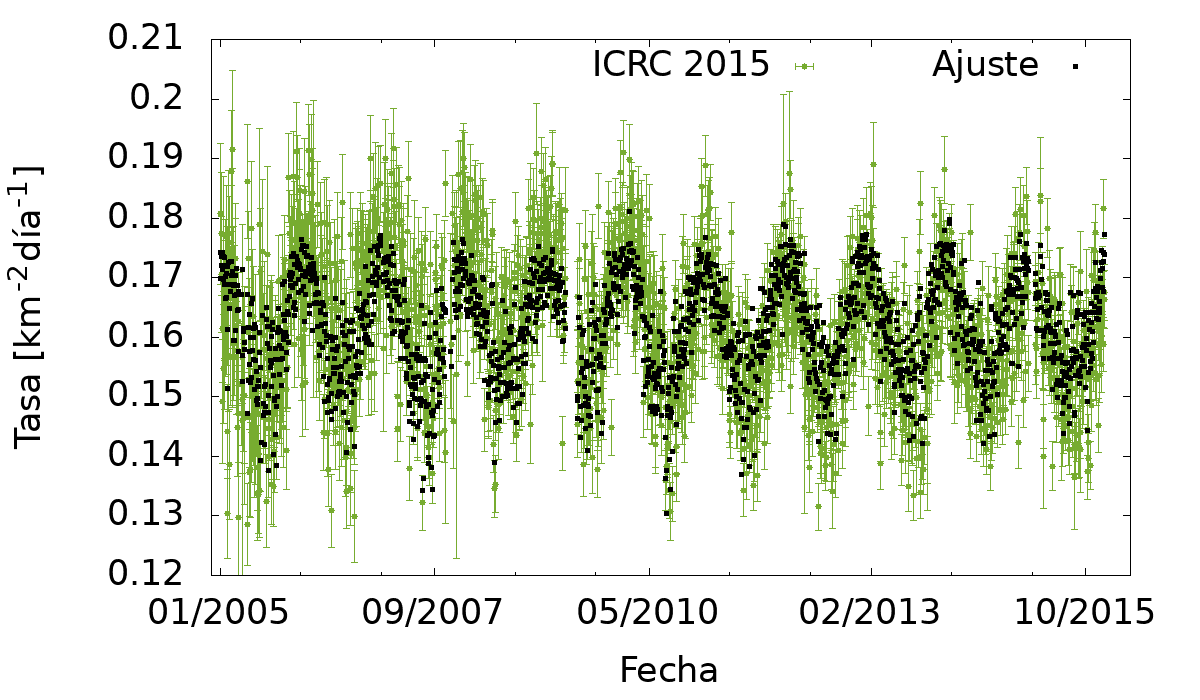
\includegraphics[width=\textwidth]{Graphs/rate_dayly/1EeV_ICRC_2015.png}
				\caption{Tasa eventos por día}\label{fig:rate_dayly_ICRC_2015}
    			\end{subfigure}%
    			\hspace{\fill}
    			\begin{subfigure}[b]{0.5\textwidth}
				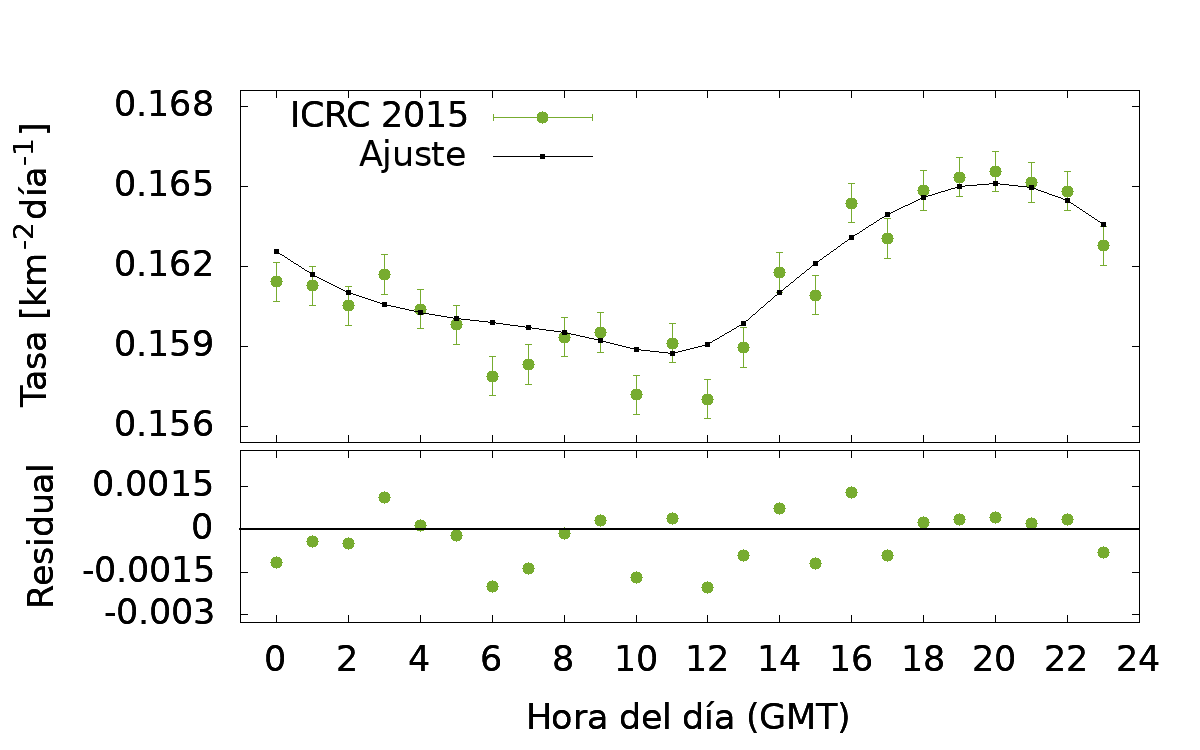
\includegraphics[width=\textwidth]{Graphs/rate_hour_of_the_day/1EeV_ICRC_2015_old_herald.png}
				\caption{Tasa de eventos promediada por hora del día }\label{fig:rate_hod_ICRC_2015}
    			\end{subfigure}%
				\caption{Tasa de eventos por días comparadas con el ajuste entre los años 2005 hasta 2015. Los datos analizados fueron los presentados en la ICRC 2015 para energías mayores a $1\,$EeV donde se observa la modulación anual y diaria del clima. }\label{fig:rate_2015_05-15}
			\end{figure}



			\begin{figure}[H]
				\begin{subfigure}[b]{0.5\textwidth}
				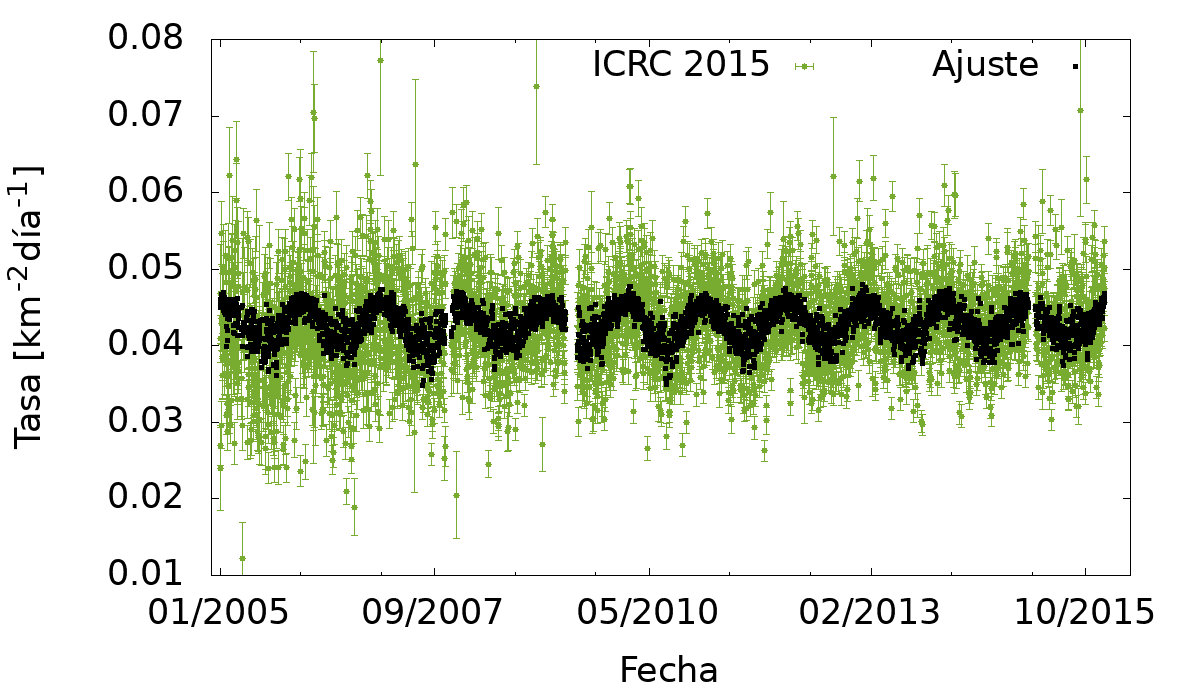
\includegraphics[width=\textwidth]{Graphs/rate_dayly/2EeV_ICRC_2015.png}
				\caption{Tasa eventos por día}\label{fig:rate_dayly_ICRC_2015_2EeV}
    			\end{subfigure}%
    			\hspace{\fill}
    			\begin{subfigure}[b]{0.5\textwidth}
				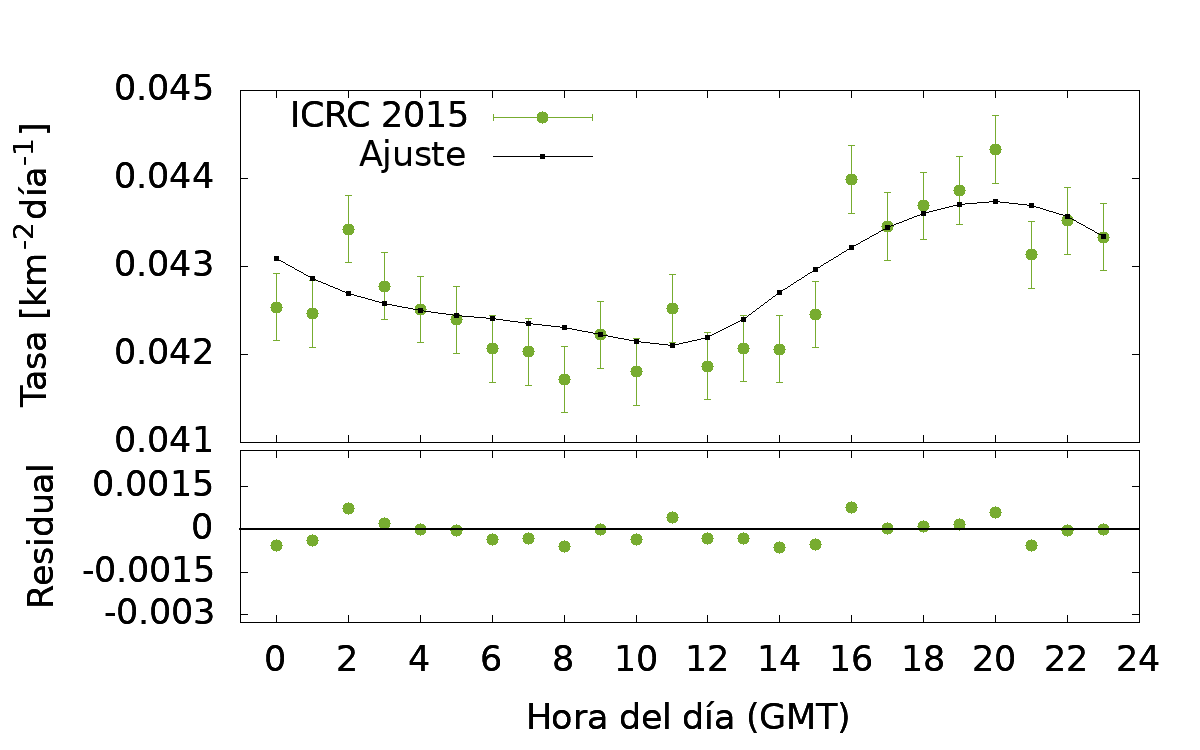
\includegraphics[width=\textwidth]{Graphs/rate_hour_of_the_day/2EeV_ICRC_2015_old_herald.png}
				\caption{Tasa de eventos promediada por hora del día }\label{fig:rate_hod_ICRC_2015_2EeV}
    			\end{subfigure}%
				\caption{Tasa de eventos por días comparadas con el ajuste entre los años 2005 hasta 2015. Los datos analizados son los presentados en la ICRC 2015 para energías mayores a $2\,$EeV. donde se observa la modulación anual y diaria del clima }\label{fig:rate_2015_05-15_2EeV}
			\end{figure}

	Como se menciona en la sección \ref{seccion:sd_eff}, el detector alcanza su máxima eficiencia para energías mayores que 3\,EeV. A partir una energía de $2\,$EeV, los eventos tienen una mayor susceptibilidad al disparo de tres tanques, mínimo número necesario para la reconstrucción de un evento. Para el conjunto A, como se muestra en la Fig.\,\ref{fig:rate_2015_05-15_2EeV}, la modulación del clima aún es apreciable para una energía mayor a $2\,$EeV. 
%====|====|	Weather params
			\subsubsection{Ajuste de los parámetros del clima}
			En esta sección se estudia la dependencia de los parámetros del clima con el ángulo cenital. Clasificamos los eventos en distintos subconjuntos según el valor de $sin^2(\theta)$ para realizar un ajuste análogo al presentado en la Tabla \ref{tabla:parametros_ICRC_2015}. Se clasifica mediante este valor para obtener números de eventos similares para cada subconjunto. Estos ajustes son presentados en las Figs. \ref{fig:ap_2015}, \ref{fig:arho_2015} y \ref{fig:brho_2015}. Los mismos se comparan con los datos presentados en \cite{aab2017impact}, usados actualmente en la corrección de los datos del Observatorio Pierre Auger. Se observa que los ajustes hechos sobre el conjunto A son compatibles con los ajustes realizados en  el trabajo \cite{aab2017impact}. 
%====|====|====|	ap, arho, brho 2005-2015 vs JINST over 1 EeV
					\begin{figure}[H]
        				\begin{subfigure}[b]{0.5\textwidth}
        				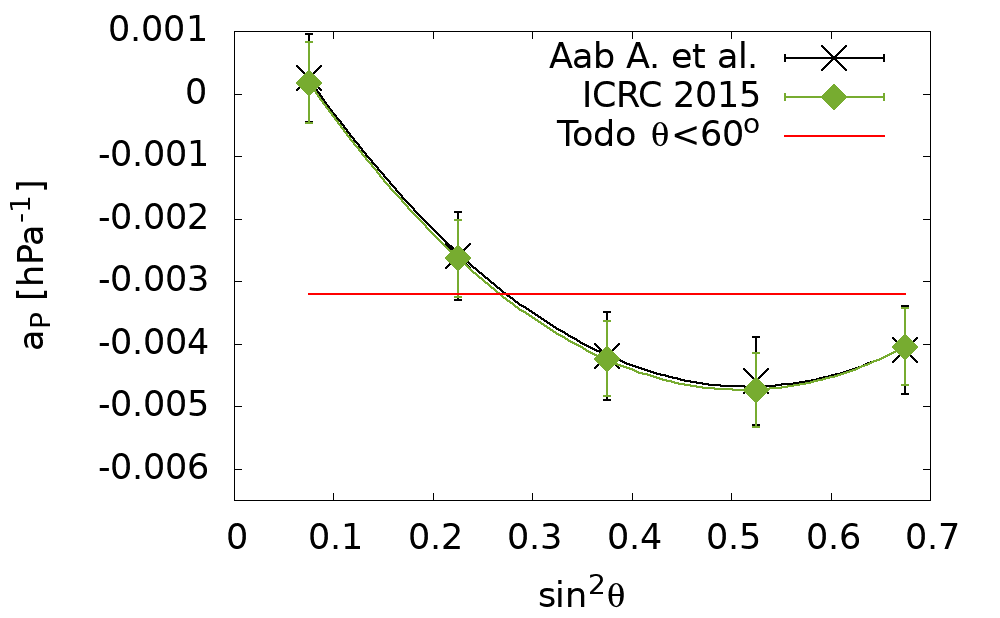
\includegraphics[width=\linewidth]{Graphs/params/ap_ICRC_2015_above_1EeV.png}
						\caption{Parámetro $a_P$ }
						\label{fig:ap_2015}
        				\end{subfigure}%
        				\hspace{\fill}
        				\begin{subfigure}[b]{0.5\textwidth}
        				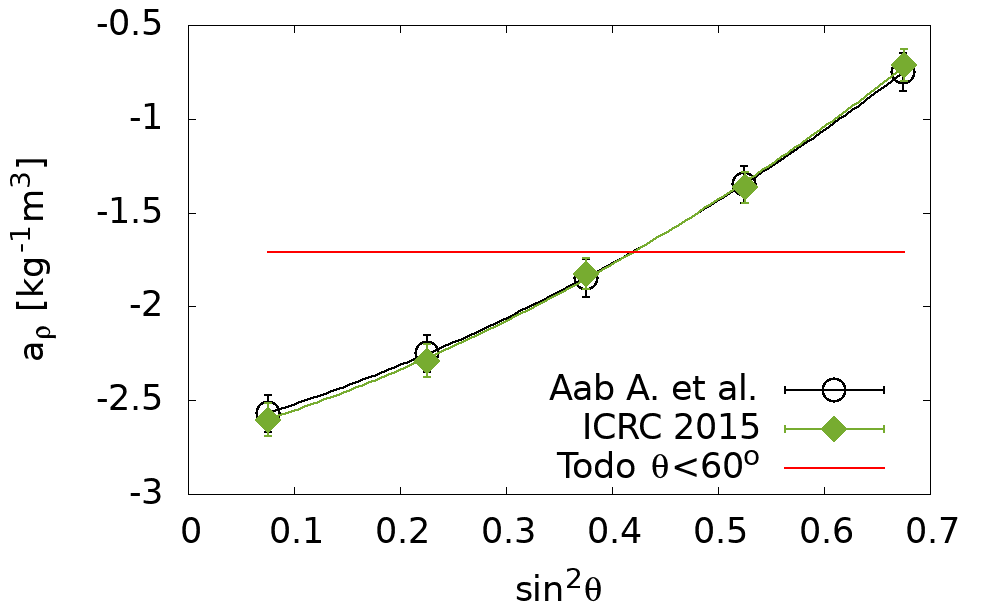
\includegraphics[width=\linewidth]{Graphs/params/arho_ICRC_2015_above_1EeV.png}
						\caption{Parámetro $a_{\rho}$ }
						\label{fig:arho_2015}
        				\end{subfigure}%
        				\hspace{\fill}
        				\begin{subfigure}[b]{\textwidth}
        				\centering
        				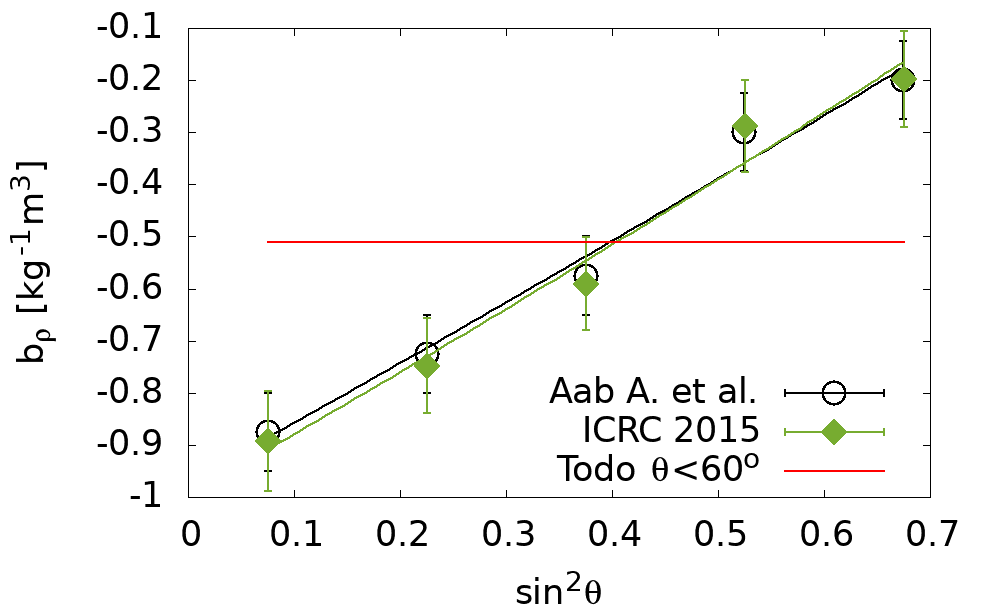
\includegraphics[width=0.5\linewidth]{Graphs/params/brho_ICRC_2015_above_1EeV.png}
						\caption{Parámetro  $b_{\rho}$	 }
						\label{fig:brho_2015}
        				\end{subfigure}%
        				\caption{Parámetros de la modulación del clima considerando los datos de la ICRC 2015. Los mismos se comparan con los ajustes obtenidos en \cite{aab2017impact} y con los ajustes obtenidos sin considerar la dependencia con $sin^2(\theta)$. }\label{fig:parameters_old}
					\end{figure}
%====|====|====| 	Tabla de c0, c1, c2
				En la Fig. \ref{fig:parameters_old} también se compara los ajustes obtenidos considerando los datos sin clasificar por $sin^2\theta$. Se observa que existe una dependencia con el ángulo cenital correspondiente al evento. Esta dependencia fue modelada mediante una función cuadrática dada en la Ec.\,\ref{eq:cuadratica}
				\begin{equation}
					f(x) = c_0 + c_1x + c_2x^2
					\label{eq:cuadratica}
				\end{equation}
				donde $x=sin^2\theta$.  En la Tabla\,\ref{tabla:cuadratica_ICRC_2015} se comparan los coeficientes obtenidos considerando la Ec.\,\ref{eq:cuadratica} con los mismos coeficiente obtenidos en el trabajo anterior \cite{aab2017impact}. 

			La dependencia con el ángulo cenital se debe a que para distintos ángulos de incidencia la lluvia interactúa con más o menos atmósfera. Los efectos de las condiciones climáticas afectan el desarrollo de la lluvia. Por ejemplo, el coeficiente de la presión  es negativo para $\sin^2(\theta)>0.3$ o $\theta>33^o$, lo que indica que si presión sube la señal baja. Esto es una consecuencia de que la lluvia  está en un estado más avanzado de su desarrollo. Para ángulos cenitales cercanos a $60^o$, la componente electromagnética es suprimida por las interacciones en la atmósfera, por lo tanto el efecto de la presión disminuye. El resultado obtenido en la Fig.\,\ref{fig:ap_2015} es consistente con este fenómeno, dado que el valor de $a_P$ disminuye al aumentar el ángulo. 		En el caso de los coeficientes relacionados con la densidad, también se observa que los parámetros son negativos, dado que un aumento de la densidad disminuye $r_M$ y por lo tanto la extensión de la señal. Se observa también que los parámetros $a_\rho$ y $b_\rho$ tienen la misma tendencia con $\sin^2(\theta)$, además de que los coeficientes tienen una razón de aproximadamente $\nicefrac{1}{3}$, lo cual se esperaba por lo discutido en la sección \ref{seccion:fisica_clima}.
					\begin{table}[H]
						\centering
						\begin{tabular}{|l|l|l|l|}\hline
						 	Parámetros									& Coeficiente		& Este Trabajo			& \cite{aab2017impact}	\\ \hline
						 \multirow{3}{*}{$a_P$ [hPa$^{-1}$]}  			&  $c_0$			& $ 0.00200\pm 0.00005$	& $0.0021 \pm 0.0009 $	\\ \cline{2-4} %Done
						 												&  $c_1$			& $-0.0263 \pm 0.0002$	& $-0.026 \pm 0.006 $	\\ \cline{2-4} 
																		&  $c_2$			& $ 0.0257 \pm 0.0002$	& $0.026  \pm 0.007 $	\\ \hline % 
						
						 \multirow{3}{*}{$a_\rho$ [kg$^{-1}$m$^3$]}  	&  $c_0$			& $-2.73   \pm 0.05$	& $ -2.7  \pm 0.1  $\\ \cline{2-4} 
						 												&  $c_1$			& $ 1.5    \pm 0.4 $	& $ 1.5   \pm 0.8  $\\ \cline{2-4} 
																		&  $c_2$			& $ 2.1    \pm 0.7 $	& $ 2.2   \pm 1.0  $\\ \hline %
						
						\multirow{3}{*}{$b_\rho$ [kg$^{-1}$m$^3$]} 		&  $c_0$			& $-1.0    \pm 0.1$		& $-1.0   \pm 0.1 $	\\ \cline{2-4} 
																		&  $c_1$			& $ 1.2    \pm 0.6$		& $ 1.2   \pm 0.8  $	\\ \cline{2-4} 
																		&  $c_2$			& $ 0.1    \pm 0.8$		& $ 0.0   \pm 1.1  $	\\ \hline 
						
						\end{tabular}	
						\caption{Tabla de los coeficientes obtenidos para el conjunto de datos de la ICRC 2015, comparados con el trabajo anterior \cite{aab2017impact}} \label{tabla:cuadratica_ICRC_2015}
					\end{table}

%==================================================================================================================
%==================================================================================================================
%==================================================================================================================
%==================================================================================================================

%====|==> ICRC 2019
	 \subsection{Datos presentados en la ICRC 2019}\label{conjuntoB}
	 	Comparando este conjunto de datos con los datos de la ICRC 2015, los datos de la ICRC 2019 contienen eventos de los tres años posteriores. Posterior al trabajo \cite{aab2017impact}, la señal de S(1000) fue corregida por las condiciones climáticas en la reconstrucción oficial de eventos. Además el valor de S(1000) estimado para cada evento cambió entre estos dos conjuntos de datos, por parte de la reconstrucción oficial \cite{isabel}. Se realizó también una nueva calibración de la energía mediante eventos híbridos, como la mostrada en la Fig.\,\ref{fig:efd_s38} en el trabajo  \cite{tobepublished}. En el conjunto de datos de la ICRC 2019, se realizó los mismos cortes que para el conjunto de A de la sección anterior. En el periodo 2005-2015 de los datos de la ICRC 2019 con los cortes mencionados de energía mayor a $1\,$EeV para eventos verticales, la cantidad de eventos con energías mayores a $1\,$EeV subió de 1146470 a  1280918 eventos. Esto puede deberse a la corrección del clima de los eventos, donde aquellos eventos que estaban por debajo del corte del energía, tras la corrección pudieron estar por encima de este corte. Otro posibilidad es la nueva reconstrucción haya aumentado la cantidad de eventos por encima de $1\,$EeV. Por eso la media de energía bajó de $2.00\,$EeV a $1.91\,$EeV.  Las características de los datos en estos dos rangos de tiempo se resumen en la Tabla\,\ref{tabla:caracteristicas_ICRC_2019}. 
%====|====|	Tabla de eventos exposure
			\begin{table}[H]
				\centering
				\begin{tabular}{|c|c|c|}
				\hline
				\textbf{Tiempo }    & \textbf{01/01/2005-31/12/2015}  & \textbf{01/01/2005-31/12/2018 }\\ \hline 
				%Exposición          &          				 &          			\\ \hline
				Número de eventos   &  1280918     			 &  1635045     		 \\ \hline 
				Energía media       &  1.91				 &	1.92				\\ \hline % 1.0734        		 &  1.1370       			\\ \hline 
				Corte en energía    &  1 EeV       		 	 &  1 EeV       		 \\ \hline 
				Ángulo cenitales	&  $60^o$ 				 & $60^o$\\ \hline
				\end{tabular}
				\caption{Características de los datos de la ICRC 2019 utilizados para los ajustes de esta sección.} \label{tabla:caracteristicas_ICRC_2019}
			\end{table}

			En la Fig.\,\ref{fig:rate_new_18} se muestran las tasas de eventos por día para energía mayores a $1\,$EeV y $2\,$EeV, con la energía corregida por los efectos climáticos según la reconstrucción oficial \cite{data}. En la Fig.\,\ref{fig:rate_new_18_2EeV} se  comparan con los resultados de los datos de la ICRC 2015, la modulación en la tasa ya no es apreciable. Si comparamos las tasas de eventos por hora del día de los eventos por encima de $1\,$EeV y $2\,$EeV, por encima de $1\,$EeV, se aprecia un remanente de la modulación del clima diaria comparado con la tasa para $2\,$EeV. Esto se debe a que el SD tiene eficiencia para energía mayores a $3\,$EeV, comentado anteriormente.


				Existe una modulación remanente en la tasa de eventos como se aprecia en las Figs.\,\ref{fig:rate_day_ICRC_19_05_18} y \ref{fig:rate_day_ICRC_19_05_18_2EeV}. Esto se debe que la señal es mayor que la esperada como consecuencia de las condiciones atmosféricas en el momento del evento, por lo tanto la eficiencia del disparo ante este evento también es mayor. De esta forma la eficiencia tiene una dependencia con las condiciones atmosféricas.
%====|====|	2005-2019	rate day over 1 EeV
%====|====|	2005-2019	rate hour of the day	1 EeV
			\begin{figure}[H]
    			\begin{subfigure}[b]{0.5\textwidth}
				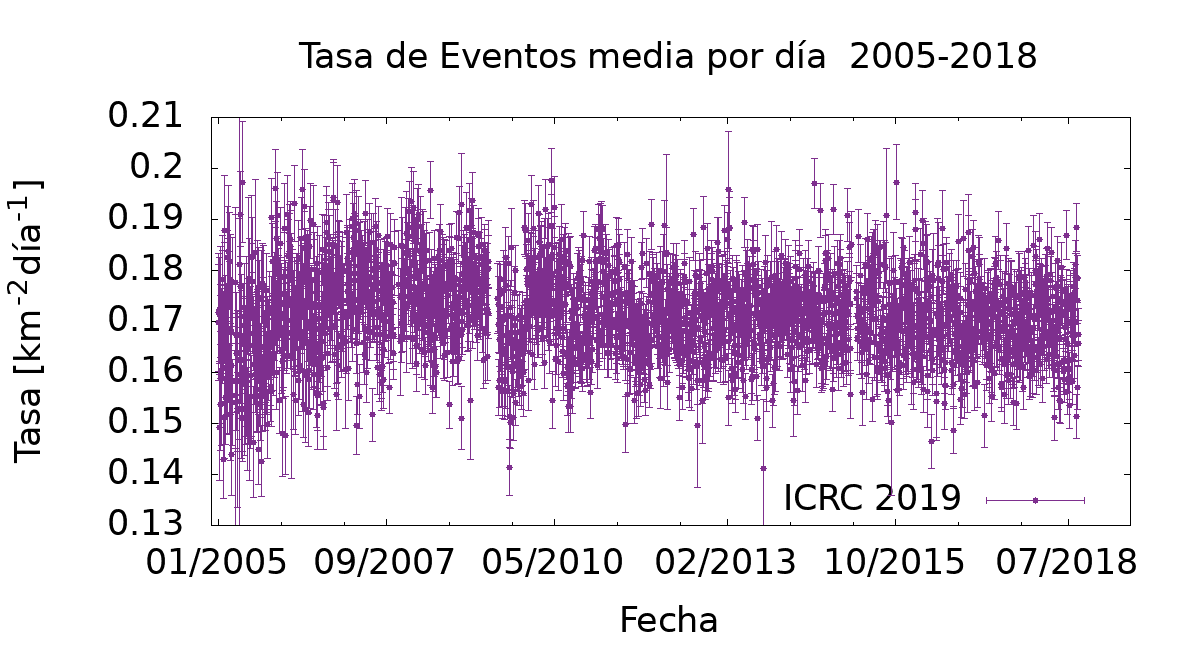
\includegraphics[width=\textwidth]{Graphs/rate_dayly/1EeV_ICRC_2019_05_18.png}
				\caption{Energía mayor a $1\,$EeV}
				\label{fig:rate_day_ICRC_19_05_18}
    			\end{subfigure}%
    			\hspace{\fill}
    			\begin{subfigure}[b]{0.5\textwidth}
				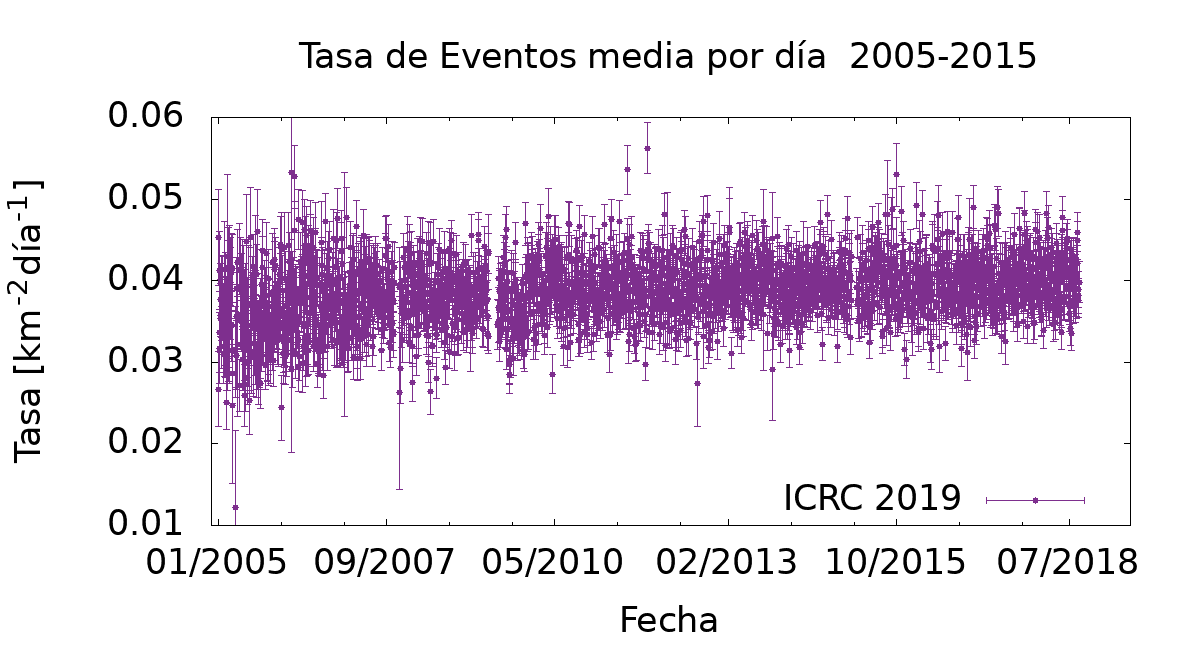
\includegraphics[width=\textwidth]{Graphs/rate_dayly/2EeV_ICRC_2019_05_19.png}
				\caption{ Energía mayor a $2\,$EeV}
				\label{fig:rate_2015_ICRC_19_05_18}
    			\end{subfigure}%
    			\caption{Tasa de eventos promedio por cada día entre los años 2005 hasta 2015 del conjunto de datos presentado en la ICRC 2019. Se muestran las tasas para dos cortes en energía, mayor a $1\,$EeV y mayor a $2\,$EeV}\label{fig:rate_new_18}
			\end{figure}
			\begin{figure}[H]
    			\begin{subfigure}[b]{0.495\textwidth}
				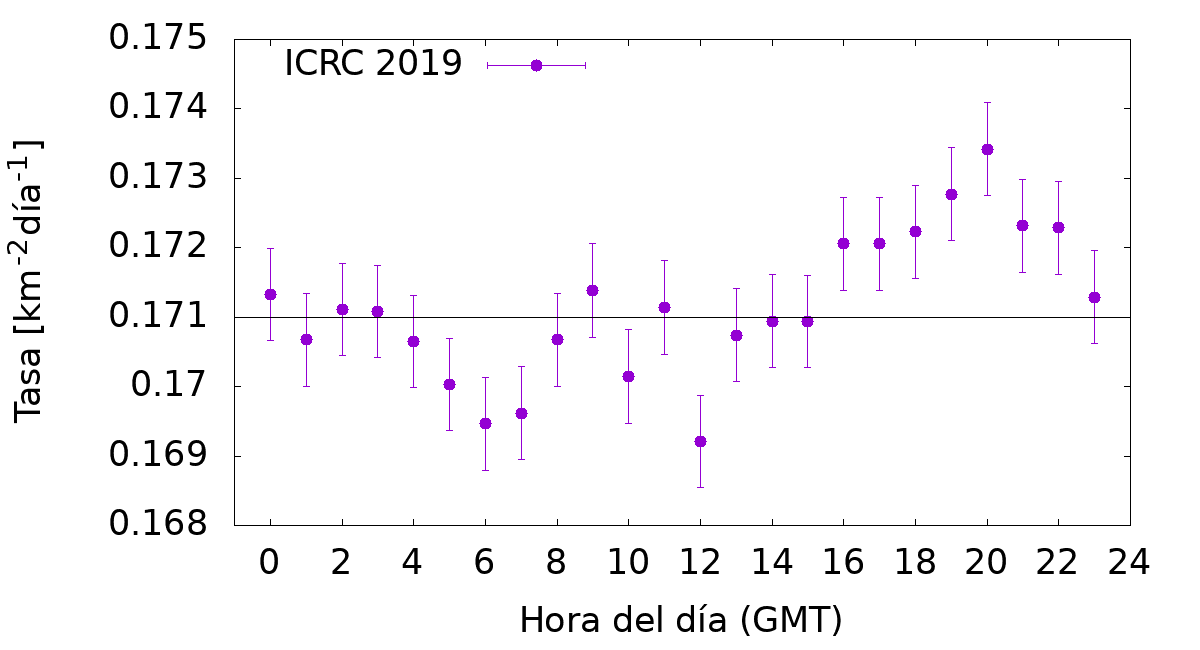
\includegraphics[width=\textwidth]{Graphs/rate_hour_of_the_day/1EeV_ICRC_2019_05_19.png}
				\caption{Energía mayor a $1\,$EeV}
				\label{fig:rate_day_ICRC_19_05_18_2EeV}
    			\end{subfigure}%
    			\hspace{\fill}
    			\centering
    			\begin{subfigure}[b]{0.495\textwidth}
				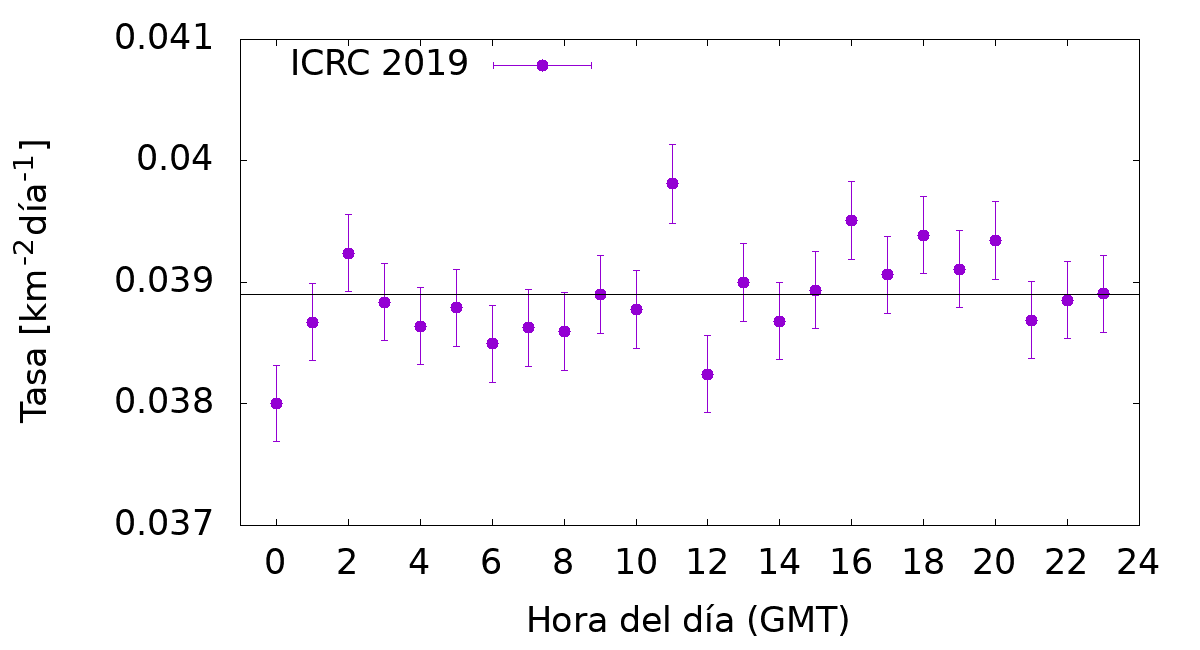
\includegraphics[width=\textwidth]{Graphs/rate_hour_of_the_day/2EeV_ICRC_2019_05_18.png}
				\caption{Energía mayor a $2\,$EeV}
				\label{fig:rate_2015_ICRC_19_05_18_2EeV}
    			\end{subfigure}%
    			\caption{Tasa eventos  por hora del día por unidad de área entre los años 2005 hasta 2015 del conjunto de datos presentado en la ICRC 2019.  Se muestran las tasas para dos cortes en energía, mayor a $1\,$EeV y mayor a $2\,$EeV}\label{fig:rate_new_18_2EeV}
			\end{figure}


	
%====|==>ICRC 2019 S$_{38}$-Sin Corrección
	\subsection{Datos presentados en la ICRC 2019 usando $S_{38}$ sin corregir por el clima}

	Además de tener más estadística de los eventos registrados, durante el periodo 2016-2018 también se recabaron datos sobre el clima en el observatorio. La modulación del clima fue estudiada anteriormente realizando un corte de la energía sin corregir. En esta sección se realiza el análisis de la modulación mediante un  corte sobre la señal medida por el SD. En el conjunto de datos de la ICRC 2019, es posible acceder al valor de S(1000) sin corregir por el trabajo \cite{aab2017impact}, por que uno puede obtener el valor de S$_{38}$ sin corregir mediante la expresión
	\begin{equation}
		S_{38} = \frac{S(1000)}{S(1000)_w}S_{38,w}
		\label{eq:s38_w}
	\end{equation}
	donde las variables $S(1000)_w$ y $S_{38,w}$ indican los valores corregidos por clima. Estas variables están listadas en el conjunto de datos presentado en la ICRC 2019. Dado que los trabajos anteriores se basaron en la energía para hacer el corte de los eventos, se realizó el corte con la señal de $S_{38}\ge 5.37\,$VEM correspondiente a 1\,EeV aproximadamente. %Mediante este corte, el análisis no tiene en cuenta las correcciones del clima y es posible obtener parámetros del clima mediante el valor de S$_{38}$. 
	Las características de este conjunto de datos están resumidos en la Tabla\,\ref{tabla:caracteristicas_ICRC_2019_S38}.
%====|====|	Tabla de eventos exposure
			\begin{table}[H]
				\centering
				\begin{tabular}{|c|c|c|}
				\hline
				\textbf{Tiempo }    & \textbf{01/01/2005-31/12/2015}  & \textbf{01/01/2005-31/12/2018 }\\ \hline 
				%Exposición          &          				 &          			\\ \hline
				Número de eventos   &   1267265     		 &  1618717     		\\ \hline 
				Energía media       &  1.89        		 	 &  1.90        		\\ \hline 
				Corte en S$_{38}$ 	    &  5.37\,VEM   		 	 &  5.37\,VEM       	\\ \hline 
				Ángulo cenital 		&  $<60^o$ 			 	 & $<60^o$\\ \hline
				\end{tabular}
				\caption{Características de los datos de la ICRC 2019 utilizados para los ajustes de esta sección.} \label{tabla:caracteristicas_ICRC_2019_S38}
			\end{table}

			%Cabe destacar que la cantidad de eventos considerados para el periodo 2005-2015 para este caso es mayor que para la ICRC 2015 en el mismo periodo. Esto se debe que tras la corrección del clima para la ICRC 2019, las energías cambiaron ligeramente, por lo que se tiene en cuenta eventos con energía reconstruida, menor a  1 EeV. Esto se aprecia en la disminución de la energía media.
			
%====|====| Tabla del fit
			Con estos eventos, se realizó un  ajuste de los parámetros del clima para todos los ángulos cenitales de la tasa del eventos por hora. Así se obtienen los coeficientes promediados por ángulo cenital. Estos parámetros son presentados en la Tabla\,\ref{tabla:parametros_ICRC_2019_S38}. Se observa que para ambos periodos estudiados los parámetros obtenidos son compatibles entre sí, además de ser compatibles con los resultados obtenidos para el periodo 2005-2015 de los datos de la ICRC 2015 y los parámetros de \cite{aab2017impact}, presentados en la Tabla\,\ref{tabla:parametros_ICRC_2015}.

			\begin{table}[H]
				\centering
				\begin{tabular}{|c|c|c|}
				\hline
				\textbf{Parámetro}          & \textbf{2005-2015}    		& \textbf{2005-2018}    \\ \hline
				$a_P$ [hPa$^{-1}$]          & $ -0.0033\pm 0.0003$      	& $ -0.0032\pm 0.0002$  \\ \hline
				$a_\rho$ [kg$^{-1}$m$^3$]   & $ -1.75\pm 0.04$            	& $ -1.71\pm 0.03$       \\ \hline
				$b_\rho$ [kg$^{-1}$m$^3$]   & $ -0.51\pm 0.04$             	& $ -0.52\pm 0.03$       \\ \hline
				$\chi^2_\nu$                & $1.00616$                     & $1.01819$              \\   \hline
				\end{tabular} 
				\caption{Parámetros del clima obtenidos para todos los ángulos cenitales para los dos rangos de tiempo estudiados.} \label{tabla:parametros_ICRC_2019_S38}
			\end{table}
			
			Calculando la tasa de eventos esperado con los parámetros de la Tabla\,\ref{tabla:parametros_ICRC_2019_S38}, esta se comparan con la tasa experimental medida con el SD, que se muestra en la Fig. \ref{fig:rate_new_18_S38} para el rango de tiempo 2005-2018. En estos gráficos se observa que la modulación del clima tiene la mismas características que las observadas en la sección \ref{icrc2015}.

			\begin{figure}[H]
    			\begin{subfigure}[b]{0.5\textwidth}
				\includegraphics[width=\textwidth]{Graphs/rate_dayly/0EeV_ICRC_2019_S38_05_18.png}
				\caption{Tasa eventos por cada día por unidad de área}
				\label{fig:rate_day_ICRC_19_S38_05_18}
    			\end{subfigure}%
    			\hspace{\fill}
    			\begin{subfigure}[b]{0.5\textwidth}
				\includegraphics[width=\textwidth]{Graphs/rate_hour_of_the_day/0EeV_ICRC_2019_S38_05_18.png}
				\caption{Tasa de eventos promedio por hora del día}
				\label{fig:rate_2015_ICRC_19_S38_05_18}
    			\end{subfigure}%
    			\caption{Tasa de eventos entre los años 2005 hasta 2018 del conjunto de datos presentado en la ICRC 2019.}\label{fig:rate_new_18_S38}
			\end{figure}

%====|====|	Weather params
		\subsubsection{Ajuste de los parámetros del clima}
		Se clasificó los eventos de esta sección mediante el valor de $sin^2\theta$ y se realizó el ajuste para obtener los parámetros del clima. Este ajuste se realizó en el periodo 2005-2018. Los valores obtenidos se resumen en la Tabla\,\ref{tabla:cuadratica_ICRC_2019_S38} y se  observan en la Fig.\,\ref{fig:parameters_new_S38}. Comparando estos resultados con los resultados de \cite{aab2017impact}, los eventos mediante el valor S$_{38}$  conservan la tendencia con $sin^2\theta$ que se observa en los datos de la ICRC 2015 en la Fig.\,\ref{fig:parameters_old}. Además los parámetros obtenidos mediante el corte por S$_{38}$ son comparables con los resultados obtenidos para el conjunto de datos de la ICRC 2015. Por lo que puede decirse que la modulación del clima es apreciable  hasta el día de hoy con una amplitud comparable al año 2015.
%====|====|====| ap, arho, brho 2005-2015  2005-2019 vs JINST over 1 EeV
				\begin{figure}[H]
    				\begin{subfigure}[b]{0.5\textwidth}
    				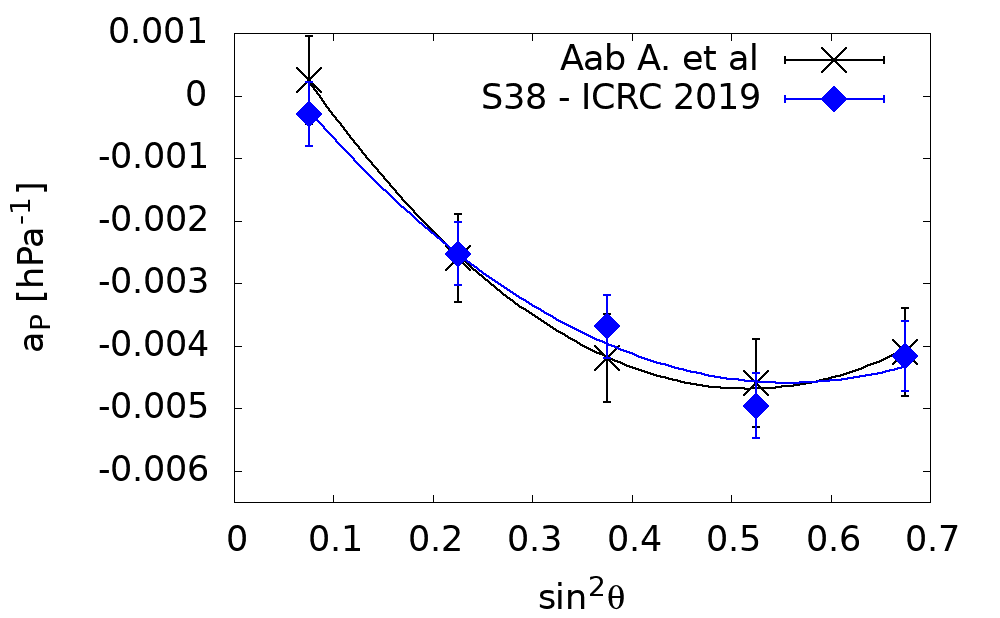
\includegraphics[width=\linewidth]{Graphs/params/ap_ICRC_2019_S38_above_0EeV.png}
					\caption{Parámetro $a_P$ }
					\label{fig:ap_2019_S38}
    				\end{subfigure}%
    				\hspace{\fill}
    				\begin{subfigure}[b]{0.5\textwidth}
    				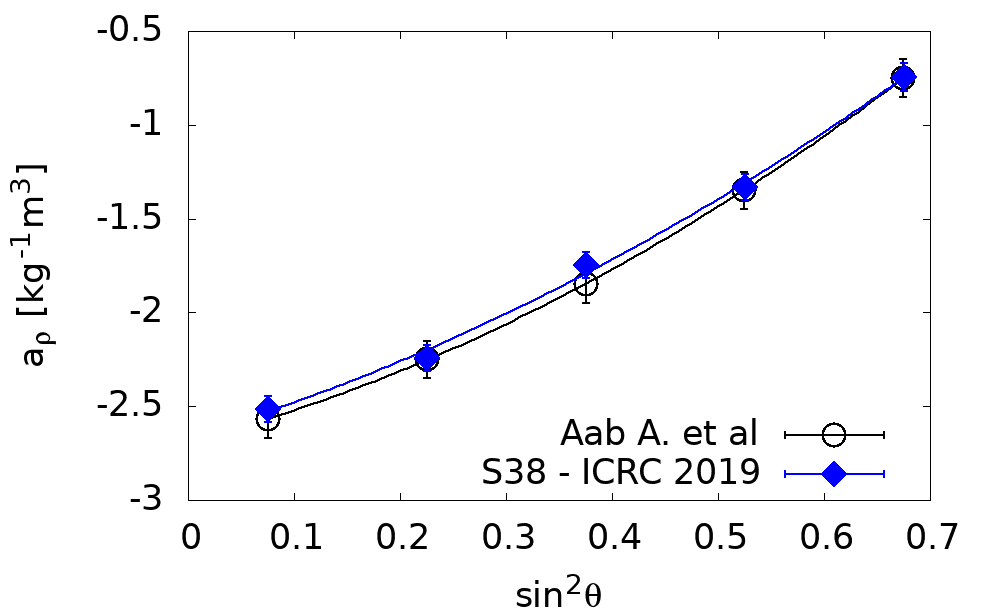
\includegraphics[width=\linewidth]{Graphs/params/arho_ICRC_2019_S38_above_0EeV.png}
					\caption{Parámetro $a_{\rho}$ }
					\label{fig:arho_2019_S38}
    				\end{subfigure}%
    				\hspace{\fill}
    				\begin{subfigure}[b]{\textwidth}
    				\centering
    				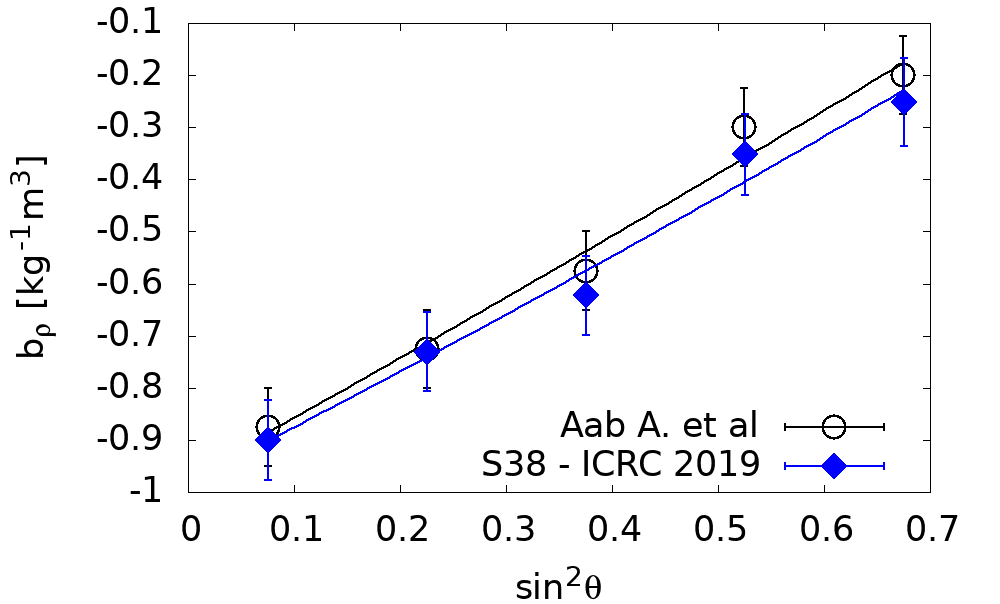
\includegraphics[width=0.5\linewidth]{Graphs/params/brho_ICRC_2019_S38_above_0EeV.png}
					\caption{Parámetro  $b_{\rho}$	 }
					\label{fig:brho_2019_S38}
    				\end{subfigure}%
    				\caption{Parámetros de la modulación del clima considerando los datos sin corregir con el clima y la reconstrucción anterior.}\label{fig:parameters_new_S38}
				\end{figure}
%====|====|====| Tabla de c0, c1, c2
					\begin{table}[H]
						\centering
						\begin{tabular}{|l|l|l|l|}\hline
						 \textbf{Parámetros}						& \textbf{Coeficiente}	& \textbf{Este Trabajo} & \textbf{ \cite{aab2017impact}}	\\ \hline
						 \multirow{3}{*}{$a_P$ [hPa$^{-1}$]}  		&  $c_0$				& $ 0.0012\pm0.0005$	& $ 0.0021 \pm 0.0009 $	\\ \cline{2-4} %Done
						 											&  $c_1$				& $-0.020\pm0.003$		& $-0.026  \pm 0.006 $	\\ \cline{2-4} 
																	&  $c_2$				& $ 0.019\pm0.004$		& $0.026   \pm 0.007 $	\\ \hline % 
						
						 \multirow{3}{*}{$a_\rho$ [kg$^{-1}$m$^3$]} &  $c_0$			& $-2.66   \pm 0.07$	& $ -2.7  \pm 0.1  $\\ \cline{2-4} 
						 											&  $c_1$			& $ 1.7    \pm 0.4 $	& $ 1.5   \pm 0.8  $\\ \cline{2-4} 
																	&  $c_2$			& $ 1.7    \pm 0.6 $	& $ 2.2   \pm 1.0  $\\ \hline %
						
						\multirow{3}{*}{$b_\rho$ [kg$^{-1}$m$^3$]} 	&  $c_0$			& $-0.98    \pm 0.08$	& $-1.0   \pm 0.1 $	\\ \cline{2-4} 
																	&  $c_1$			& $ 1.00    \pm 0.5$	& $ 1.2   \pm 0.8  $	\\ \cline{2-4} 
																	&  $c_2$			& $ 0.1    \pm 0.6$		& $ 0.0   \pm 1.1  $	\\ \hline 
						
						\end{tabular}	
						\caption{Tabla de los coeficientes obtenidos con el S$_{38}$ sin corregir por el clima, comparados con el trabajo anterior} \label{tabla:cuadratica_ICRC_2019_S38}
					\end{table}

%==================================================================================================================
%==================================================================================================================
%==================================================================================================================
%==================================================================================================================
	


%====|==>ICRC 2019 Reconstrucción con este trabajo
\subsection{Datos presentados en la ICRC 2019 usando la energía reconstruida en este trabajo}

Con el subconjunto de datos de la ICRC 2019 con los cortes utilizados en la sección anterior, se realizó una corrección del valor de S$_{38}$ con los parámetros del clima presentados en la Tabla.\,\ref{tabla:cuadratica_ICRC_2019_S38}. Con este valor corregido se calculó la energía corregida mediante la Ec.\,\ref{eq:s38_energy}. Para una energía mayor de $2\,$EeV, se espera que los efectos del clima sean despreciables tras la corrección, porque se acerca a la eficiencia máxima de los detectores de superficie. El método de CIC está determinado usando los eventos donde el SD tiene un eficiencia máxima, evitando la susceptibilidad del disparo de los detectores.

En la Fig.\,\ref{final} se comparan los tasas de eventos por hora del día para el conjunto de datos de la ICRC 2019 y para la corrección de energía realizada en este trabajo. En la figura superior se muestra la tasa de eventos por hora del día del conjunto de datos de la sección \ref{conjuntoB}, comparada con la tasa de eventos para la energía corregida por este trabajo, presentada en la figura inferior. En ambos casos corrección queda plana, eliminando el error sistemático de la modulación del clima.
			\begin{figure}[H]
    				\begin{subfigure}[b]{0.5\textwidth}
					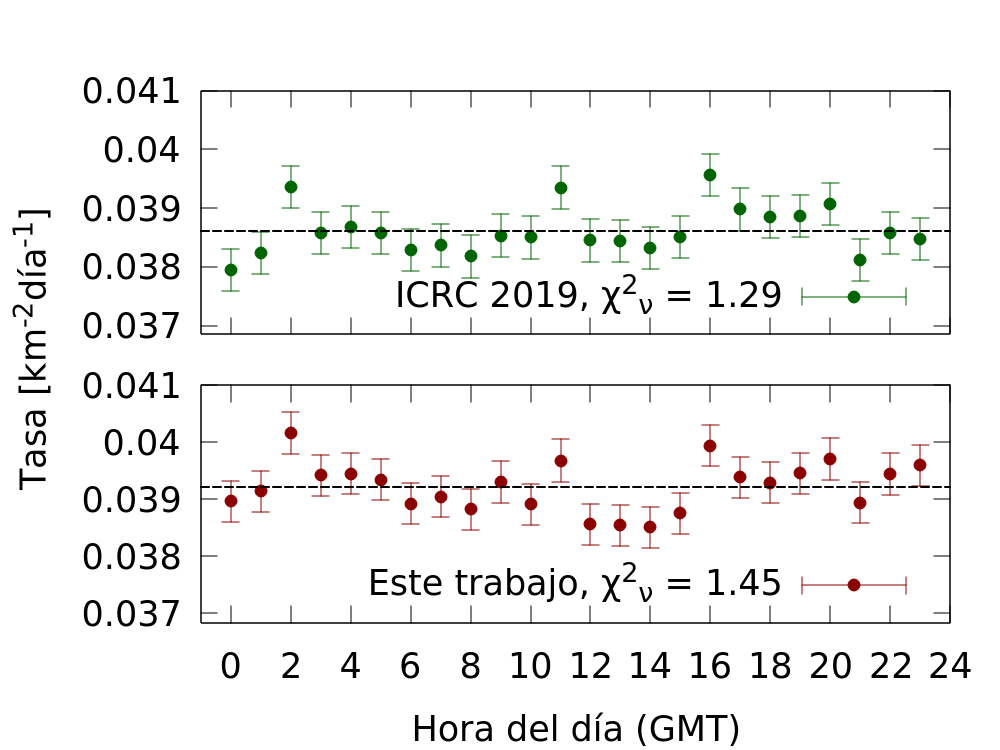
\includegraphics[width=\textwidth]{Graphs/2EeV_ICRC_2019_S38_S1000_expected.png}
					\caption{2005-2015} \label{fig:2EeV_expected}
    				\end{subfigure}%
    				\hspace{\fill}
    				\begin{subfigure}[b]{0.5\textwidth}
					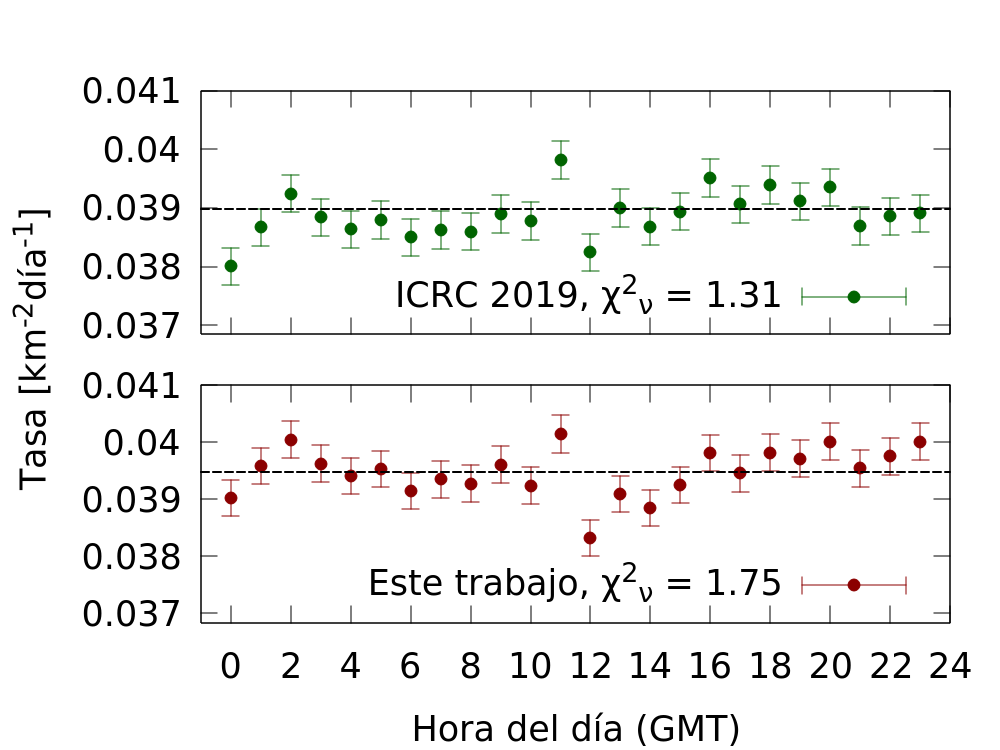
\includegraphics[width=\textwidth]{Graphs/2EeV_ICRC_2019_S38_S1000_expected_05_18.png}
					\caption{2005-2018}\label{fig:2EeV_expected_05_18}
					\end{subfigure}%
					\caption{Tasa de eventos por día para eventos de energía mayor a 2\,EeV para los datos de ICRC 2019 y la tasa de eventos obtenida con la reconstrucción de energía en este trabajo comparados en los periodos estudiados}\label{final}
			\end{figure}
Cabe aclarar que para la corrección de la energía para este trabajo, no se consideraron las posibles modulaciones de los valores del CIC o del posible cambio en los coeficientes de la Ec.\ref{eq:s38_energy}. Debido a que estos coeficientes son calibrados con eventos híbridos, que son detectados durante la noche, donde las condiciones atmosféricas difieren de las condiciones promedios. Por ejemplo, en el caso de la densidad, durante la noche es aproximadamente $2\%$ mayor que el promedio.


\section{Trabajos futuros}

Vimos que las modulaciones del clima son parametrizadas mediante los coeficientes obtenidos en este y en otros trabajos de manera precisa. Durante la maestría se realizará un análisis de anisotropía con las energías corregidas por las condiciones atmosféricas mediante este trabajo y \cite{aab2017impact}. 
Se analizará para distintos intervalos de energía por encima de 1 EeV, el primer armónico de ascensión recta en frecuencia solar y anti-sidérea, usando las  dos correcciones mencionadas. En estas dos frecuencias la señal debería ser menor a las fluctuaciones estadísticas, si las modulaciones espurias debidas a las condiciones atmosféricas están corregidas correctamente. En ese caso se puede realizar un análisis de Fourier estándar en la frecuencia sidérea para estudiar las anisotropías a grandes escalas angulares.

%Se cuantificará las comparaciones entre las correcciones de \cite{aab2017impact} y de este trabajo, en intervalos por encima de 1\,EeV de energía, con el primer armónico en la ascensión recta en la frecuencia sidérea y anti-sidérea. Para este rango de energía también se estudiará la probabilidad de disparo de los tanques. 


Por otra parte se analizarán las correcciones del clima en la estimación de la energía para los eventos reconstruidos  utilizando los disparos $ToTd$ y $Mop$,  que permiten detectar CRs de menor energía y dan lugar a un eficiencia máxima de disparo hasta  energías del orden de $1\,$EeV. Se comprobará si los parámetros del trabajo \cite{aab2017impact} son los adecuados  para estos eventos. Luego se estudiará la amplitud del primer armónico en la frecuencia solar y anti-sidérea para comprobar la ausencia de fluctuaciones espurias, antes de realizar análisis de anisotropía. 



%FAlta cuatificar ela comparacione entre los correcione ant y ahora es un estuidar en bins encima de un 1EeV de enrgía las anisotropias / EL primer armonico en la asencrecion recta en la freq sid y anti-sie

%Para ! está la probablilidad de trigger

%El paso sigu en primer lugar mirar los triggger nuevos ToTd mops ara ver si la corrcion si la correcion de l wea ant va bien para esos evenots y de nuevo constatar como funciona siendo el pr Ra en freq sid solar, para poder usar la anisotropia intrinsieca .
 
%Empezar a hacer analisis de anisotoropia con las dos correcciones
%Arriba de 2EeV. 
%abajo de full eff hay que ponerle una ocrecicion que dpende de la eff en fun de  E y ang
%tigger nueov con full detectas mas bajo pero menos estadistica
%hacer de  una corrcion con el mops con la effic. el tema es que la ef depende del error.
%

\chapter{Anisotropías en las direcciones de arribo de los rayos cósmicos}
	
% INTRODUCCION
	\section{Introducción}
		Puedo hablar lo que puse al final de mi presentación de la tesis.

% METODOS
	\section{Métodos}

	\subsection{Exposición del detector}

	Si consideramos la variación de la exposición del observatorio durante $t_{i}$ y $t_f$, debido al crecimiento del SD o por periodos de mal funcionamiento de arreglo, modula el número de 	eventos en función del tiempo. 
	
	Para hacer el peso sigo los siguientes pasos
	\begin{enumerate}
		\item Selecciono un rango de tiempo entre $t_i$ y $t_f$.
		\item Para un periodo de tiempo $T$ en días SIDEREOS (365.25 dias normales a 366.2559 dias sidereos) , lo trasformo a  años {\bf SIDEREOS}  o vueltas, para ir barriendo las 24 hrs SIDEREAS de la ascensión recta con el periodo que estoy estudiando.
		\item Voy sumando la cantidad de tanques por cada hora que voy recorriendo. 
		\begin{equation}
			N_{tanques}(t) = \sum_j n_{tanques}(t + jT)
		\end{equation}
		\item Después de obtener las suma de los tanques , hago la ``integral'', es decir, vuelvo a sumar pero sobre las 24 horas (sidereas),  
		\begin{equation}
			I_{tanques} = \frac{1}{T} \int_{0}^{T} dt \, N_{tanques}(t) \rightarrow I_{tanques} = \sum^{288}_{t_{siderea=1}}\frac{ N_{tanques}(t_{siderea})\times5\, \text{min}}{288 \times 5\, \text{min}}
		\end{equation}
	
		\item Luego se puede calcular $\Delta N_{tanques}$ para cada hora sidérea, mediante la siguiente expresión
	
		\begin{equation}
			\Delta N_{tanques}(t) = \frac{N_{tanques}(t)}{I_{tanques}}
		\end{equation}
	
		\item Posteriormente, uno puede calcularse el peso  $w_i$ correspondiente a un evento que ocurrió a un horario (sidereo) $\tau$, mediante la siguiente expresión
		\begin{equation}
			w_i = \frac{1}{\Delta N_{tanques}(\tau)} 
		\end{equation}
		En la práctica, $\tau$ corresponde a un valor entre 0 y 287, por lo que cada intervalo de 5 min  en hora siderea tiene un peso distinto .
	
	\end{enumerate}
	
	\emph{Intenté hacerlo sin tener en cuenta y lo que sale es una convolución de frecuencia y no tengo nada físico. 20/02/2020}

	Ahora lo estoy haciendo en un span de 5 min. (24/02/2020)

	\begin{figure}[H]
		\centering
		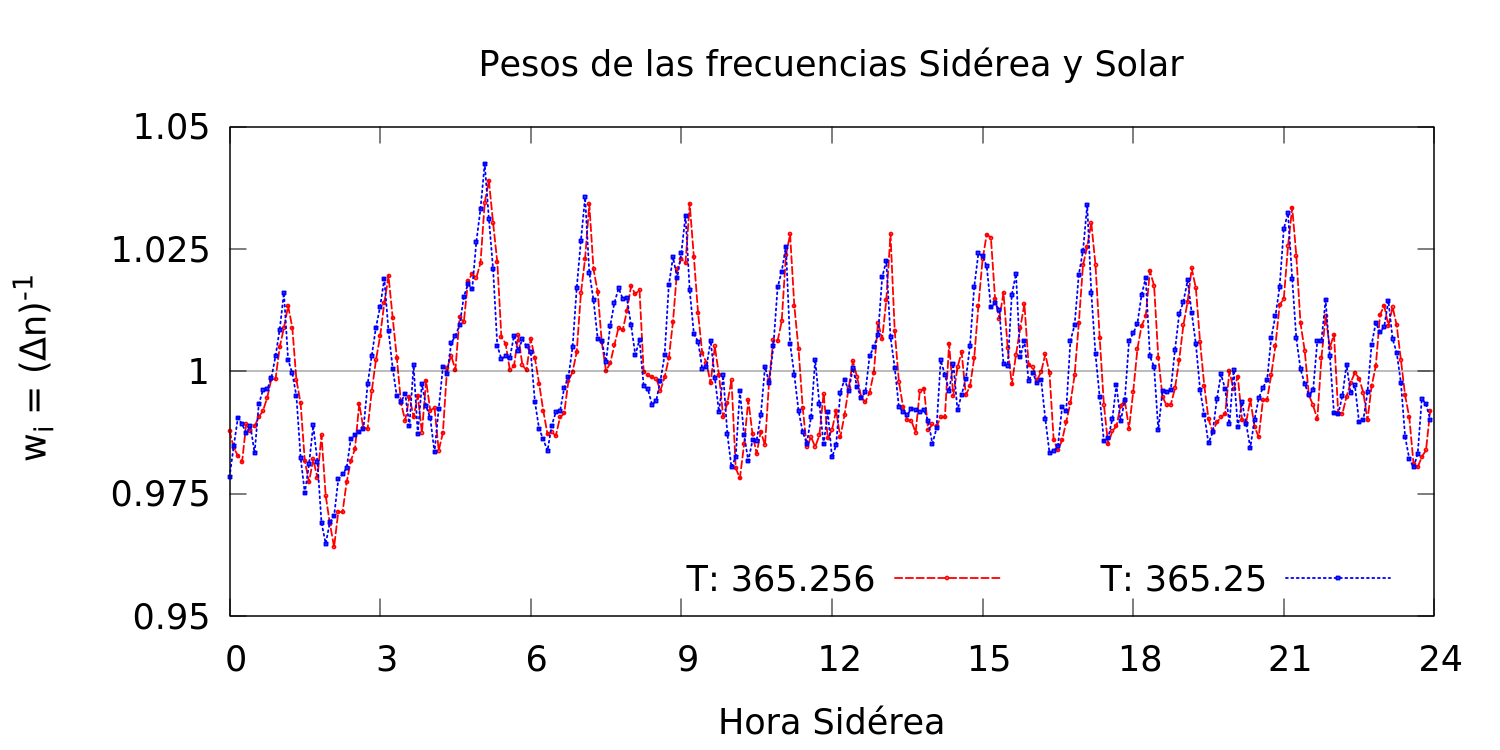
\includegraphics[width=0.95\textwidth]{pesos_solar_siderea.png}
		\caption{Pesos para dos frecuencias en particular, la frecuencia sidera y solar, de periodo $365.256$ y $365.25$ respectivamente}
		\label{fig:pesos_ejem}
	\end{figure}

	En la Fig.\ref{fig:pesos_ejem} se observa que el peso oscila alrededor de 1.

	\subsection{Análisis en ascensión recta}
	
	\begin{itemize}
		\item Ya cuando tengo los pesos $w_i$, el valor de N es $N=\sum_i w_i$
	
		\item La eficiencia del SD varía con la energía del CR. Para el disparo estandar, los eventos con energía mayor a $3\,$EeV y $\theta_{max}<60^o$ o 	por encima de $4\,$EeV y $\theta_{max}<80^o$, son detectados con una eficiencia del 100\%. Para todos los disparos, la eficiencia completa de 	alcanza por encima de 1\,EeV.
	
		\item Por lo tanto sin trabajamos con eventos donde la eficiencia es completa y sólo puede afectar el cambio de la exposición del observatorio, y  	no es necesario tener en cuenta en el peso la eficiencia.
	
		\item Para calcular el percentil 99, se usa que $P(>r) = \exp(\nicefrac{-N\,r^2}{4})$, por lo tanto para el valor de $r_{99\%}$ del percentil 99 $r	_{99\%}=\sqrt{-4\,\ln(0.01)/N}= \sqrt{4\,\ln(100)/N}$. Cabe resaltar que el P99 depende solamente de la cantidad de eventos que se se está estudiando. La interpretación 	de este valor es cual es la probabilidad de tener una amplitud mayor como una fluctuación de una distribución isotrópica.
	
		\item Para el análisis de Rayleigh, que describe el paper \cite{linsley1975fluctuation} se toma que  
		\begin{equation}
			a_\alpha = \frac{2}{N} \sum^{all}_i w_i \cos(\alpha_i)  \qquad	\qquad	b_\alpha = \frac{2}{N} \sum^{all}_i w_i \sin(\alpha_i)
		\end{equation}
	
		Donde $\alpha_i$ es el valor de la ascensión recta del evento. Para la amplitud  $r_\alpha$ y la fase $\phi_\alpha$ de cada evento
		\begin{equation}
			r_\alpha = \sqrt{a_\alpha^2 +  b_\alpha^2} \qquad \tan{\phi_\alpha} = \frac{a_\alpha}{b_\alpha}
		\end{equation}
	\end{itemize}


% ARCHIVOS DE DATOS Y SUS DIFERENCIAS
	\section{Características de los datos}

% RESULTADOS PARA ANISOTROPÍAS EN RA PARA LOS ICRC
	\section{Anisotropías en ascensión recta en los archivos del ICRC 2017 y ICRC 2019}

% ---> 8 EeV 
		\subsection{Eventos por encima de 8 EeV }

% ------> CARACTERISTICAS
			%\subsubsection{Características de los datos analizados}

% ------> ICRC 2017
			\subsubsection{Resultados para los datos del ICRC 2017}

			Para este apartado analicé el archivo de datos de la tesis de doctorado de Oscar Taborda, solamente los eventos 6T5. El rango de tiempo en el cual hice  el análisis es entre 1072969615 y 1472688000 (	2004-01-01 15:06:55 y 2016-11-01 0:00:00 )

			Sabemos que para energía mayores de 8 EeV, aparece el dipolo en sidérea.

			En las Fig.\,\ref{fig:8EeV_sin_peso_ICRC2017_raw} y \ref{fig:8EeV_sin_peso_ICRC2017_cor} se muestra la amplitud del primer armónico sin considerar el peso de los hexágonos. Está figura es compatible con la Fig. 5.7.b, página 90 de la tesis de Taborda.

				\begin{figure}[H]
				
					\begin{subfigure}[b]{\textwidth}
					\centering
						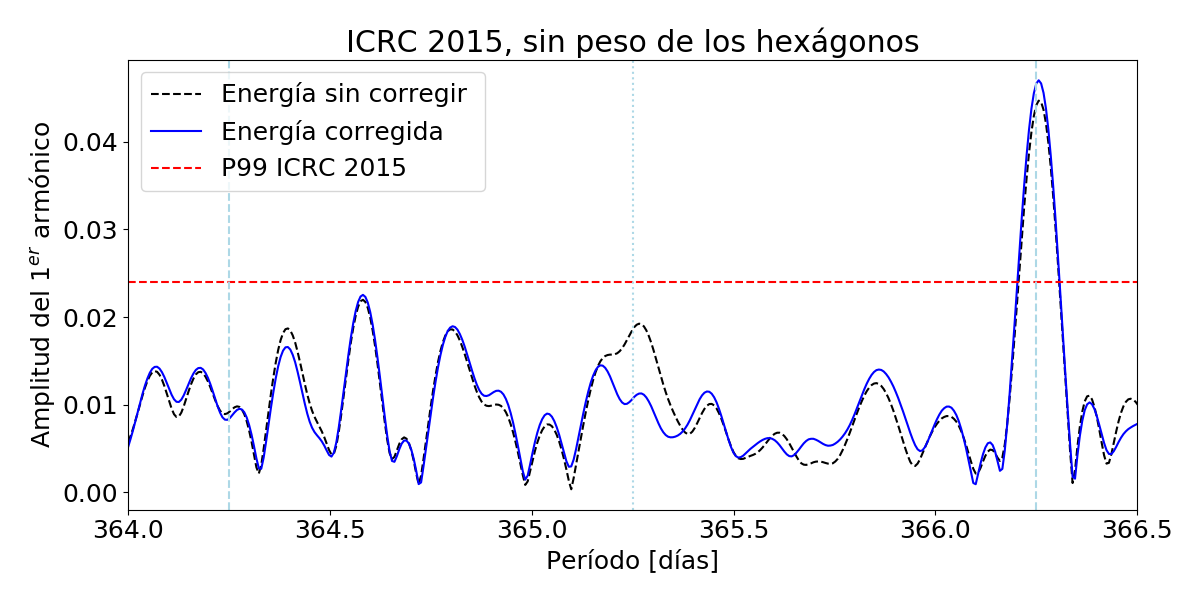
\includegraphics[width=0.6\textwidth]{ICRC/ICRC2017_Ecor_Eraw.png}
						\caption{Sin peso de la cantidad de tanques activos. } 	\label{fig:8EeV_sin_peso_ICRC2017_raw}
					\end{subfigure}%
				
					\begin{subfigure}[b]{\textwidth}
					\centering
						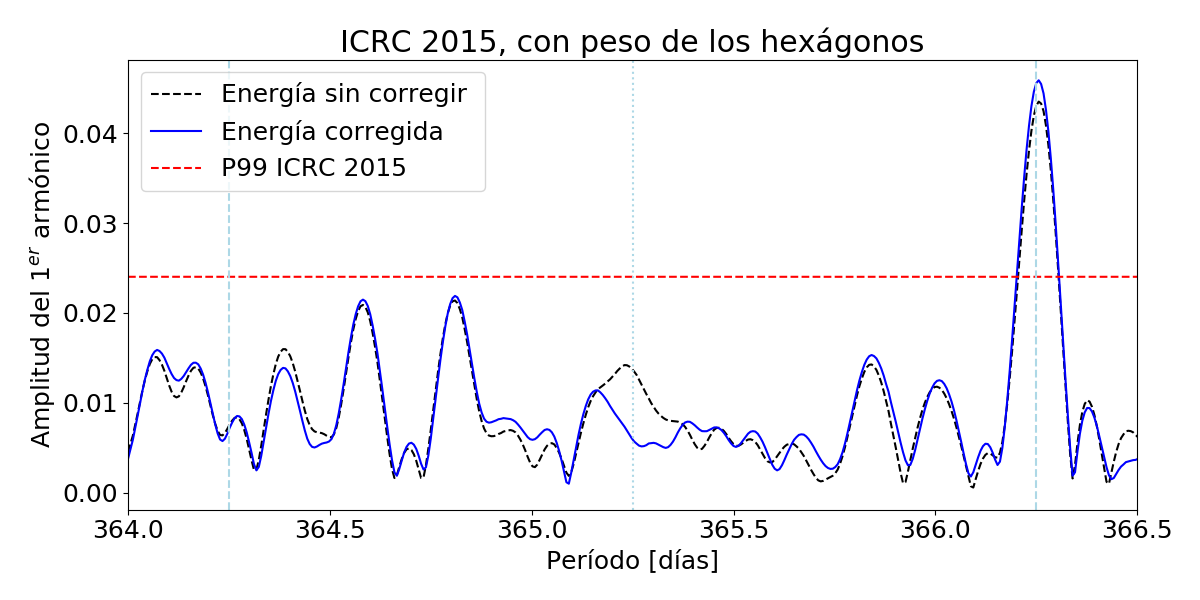
\includegraphics[width=0.6\textwidth]{ICRC/ICRC2017_Ecor_Eraw_hex.png}
						\caption{Con peso de la cantidad de tanques activos. } 	\label{fig:8EeV_sin_peso_ICRC2017_cor}
					\end{subfigure}
					\caption{Primer armónico en ascensión recta de los datos del ICRC 2017}
				\end{figure}

			Con esto podemos decir que el código para la anisotropía funciona para el caso donde no se considera los hexágonos. No tengo un referencia para comparar las anisotropías con el peso de los hexágonos, solamente el valor del pico del dipolo.

% ------> ICRC 2019
			\subsubsection{Resultados para los datos del ICRC 2019}
			
			Este es el conjunto de archivos donde se hicieron modificaciones como el uso de una nueva reconstrucción y la corrección del clima. Usé solamente los eventos 6T5. El rango de tiempo en el cual hice  el análisis es entre 1072969615 y 1535789456 (	2004-01-01 15:06:55 y 	2018-09-01 08:10:56)

			\begin{figure}[H]
				\centering
				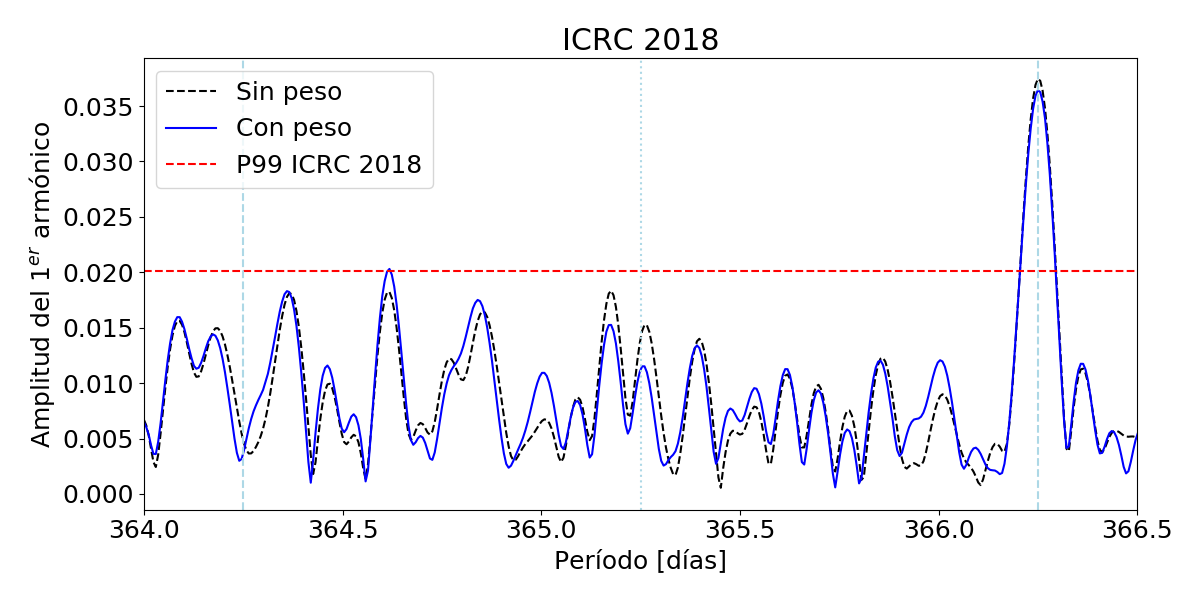
\includegraphics[width=0.6\textwidth]{ICRC/ICRC2019_Eraw_Eraw_hex.png}
				\caption{Primer armónico en ascensión recta de los datos del ICRC 2019.} \label{fig:8EeV_con_peso_ICRC2019}
			\end{figure}


			
% RESULTADOS PARA ANISOTROPÍAS EN RA PARA ALL TRIGGERS
	\section{Anisotropías en ascensión recta en los archivos con todos los disparos}
% ---> CARACTERISTICAS
		\subsection{Características de los archivos de datos analizados}

			Tenemos que tener en cuenta el archivo de datos de todos los disparos es entre los años 2013 y 2019, por lo que no podemos comparar los análisis de anisotropía con el conjunto  de datos del ICRC 2019 completo. Por lo que para compararlos, voy a hacer el análisis de ambos conjuntos de datos en el mismo rango de tiempo. Voy a hacer esto para poder comparar lo que sale. 			Este rango donde se está comparando entre archivo empieza en  $utc_i = 1372699409 $.

		%CARACTERISTICAS GENERALES DE AMBOS SET DE DATOS.

			A continuación se presentan las características de los archivos estudiados, sin ningún filtro de energía, sin acotar por tiempo. 

			\begin{table}[H]
			\centering
				\begin{tabular}{c|c|c|c}
				\textbf{Archivo} & \text{Eventos} & UTC inicial &  UTC final  \\ \hline
				2020			 & 13 739 351	  &  1372680068	&  1577879983 \\
				2019			 & 	8 463 063	  &	 1372680068 &  1496318388 \\
				2017			 &	8 592 302	  &  1372680068 &  1498521517 \\
					\end{tabular}
			\end{table}
			
			Puede verse que el Archivo de 2020 tiene más eventos, y además de tener un rango de tiempo mayor que el archivo del 2017 y 2019. Los archivos 2017 y 2019  tienen $7\,072\,964$ eventos coincidentes y los archivos 2017 y 2020 tienen $6\,902\,21$ A continuación se compara la diferencia de energía y la calibración entre estos eventos.

		%COMPARANDO DELTA E ENTRE LOS DOS ARCHIVOS
			En las  Figs.\,\ref{fig:deltaE} y \ref{fig:histograma} se muestra la diferencia entre el valor de energía entre eventos coincidentes entre los archivos 2017 y 2020. Puede apreciarse que la diferencia no esta centrada 0 y no aparenta tener una modulación del clima. Por lo tanto la diferencia se debe a una reconstrucción distinta de los eventos.

					\begin{figure}[H]
						\begin{subfigure}[b]{0.5\textwidth}
							\centering
							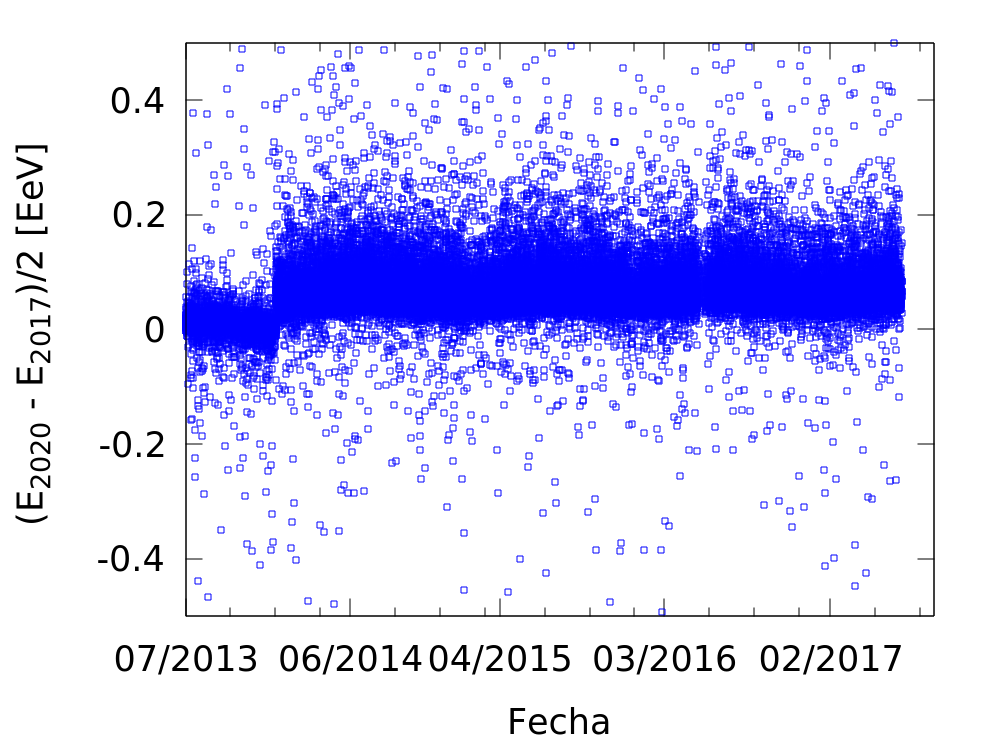
\includegraphics[width=\textwidth]{comparacion_deltaE.png}
							\caption{Diferencia entre las energías} \label{fig:deltaE}
						\end{subfigure}%
						\begin{subfigure}[b]{0.5\textwidth}
							\centering
							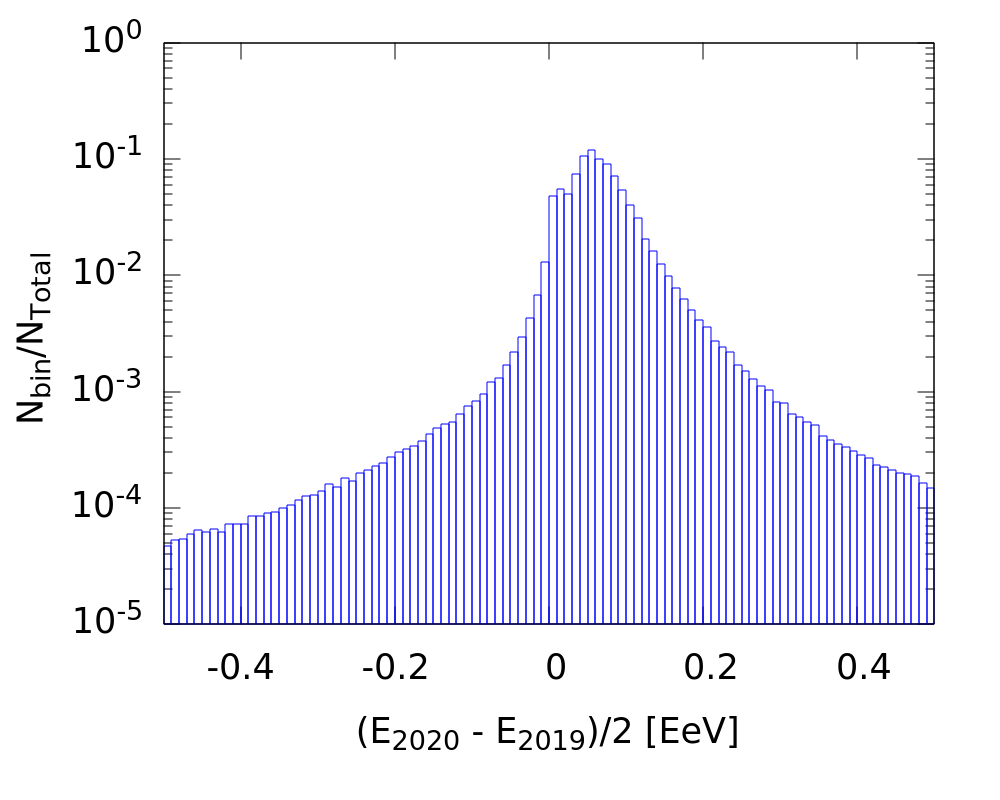
\includegraphics[width=0.8\textwidth]{histograma_deltaE.png}
							\caption{Histograma de las diferencias} 	\label{fig:histograma}
						\end{subfigure}
						\caption{Diferencia entre las energías del archivo de 2017 y el archivo del 2019}
					\end{figure}

		%COMPARANDO LA CURVA DE CALIBRACIÓN ENTRE LOS DOS ARCHIVOS
			Puede verse en la Fig.\,\ref{fig:calibracionE} que la curva de calibración entre ambos archivos es distinta, ya que la coordenada al origen como la pendiente es difieren entre para ambos archivos. Esto implica que los valores A y B de la curva $E=A\times (S_{38})^B$ son distintos para ambos conjunto de datos, ¿en qué afectaría? en primer lugar en el valor de la energía, segundo en análisis que dependan del estos parámetros como el análisis de la modulación del clima.

				\begin{figure}[H]
					\centering
					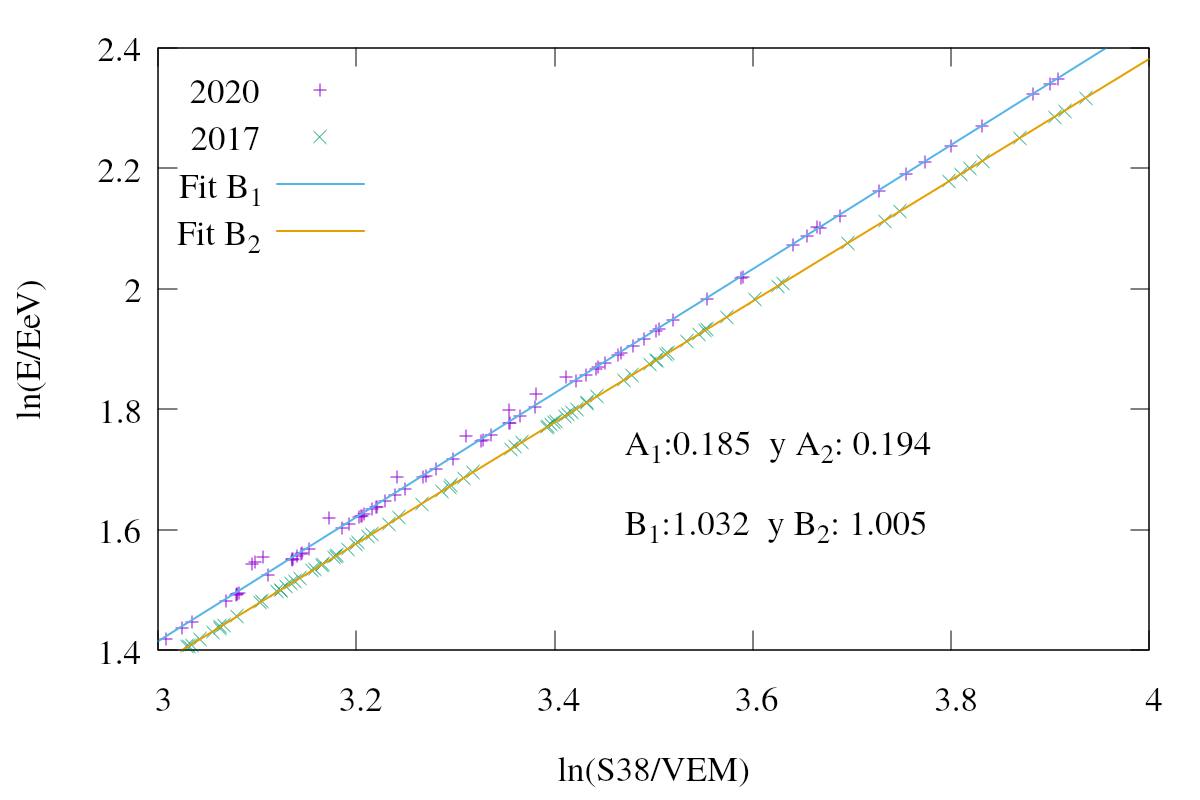
\includegraphics[width=0.65\textwidth]{comparacion_reconstruccion.png}
					\caption{Calibración de las energías del archivo de 2017 y el archivo del 2019}
					\label{fig:calibracionE}
				\end{figure}

% ---> 1 EeV 
		\subsection{Eventos por encima de 1 EeV }
% ------> CARACTERISTICAS
			\subsubsection{Características de los datos analizados}

			Comparando las cantidad de eventos por encima de 1 EeV para cada conjunto de datos

				\begin{table}[H]
					\centering
						\begin{tabular}{c|c|c|c}
						\textbf{Archivo} & \text{Eventos} 	& UTC inicial &  UTC final  \\ \hline
						2020			 & 1\,515\,872		& 1372680308  & 1577879886 \\
						%2019			 & 647\, 656		& 1372699410  & 1496267276 \\
						2017			 & 635\, 353		& 1372680308  & 1496275090 \\
						\end{tabular}
				\end{table}

{\bf hasta acá está verificado}
% ------> ALL TRIGGERS 2017
			\subsubsection{Resultados del archivo de 2017}

				\begin{figure}[H]
					\centering
					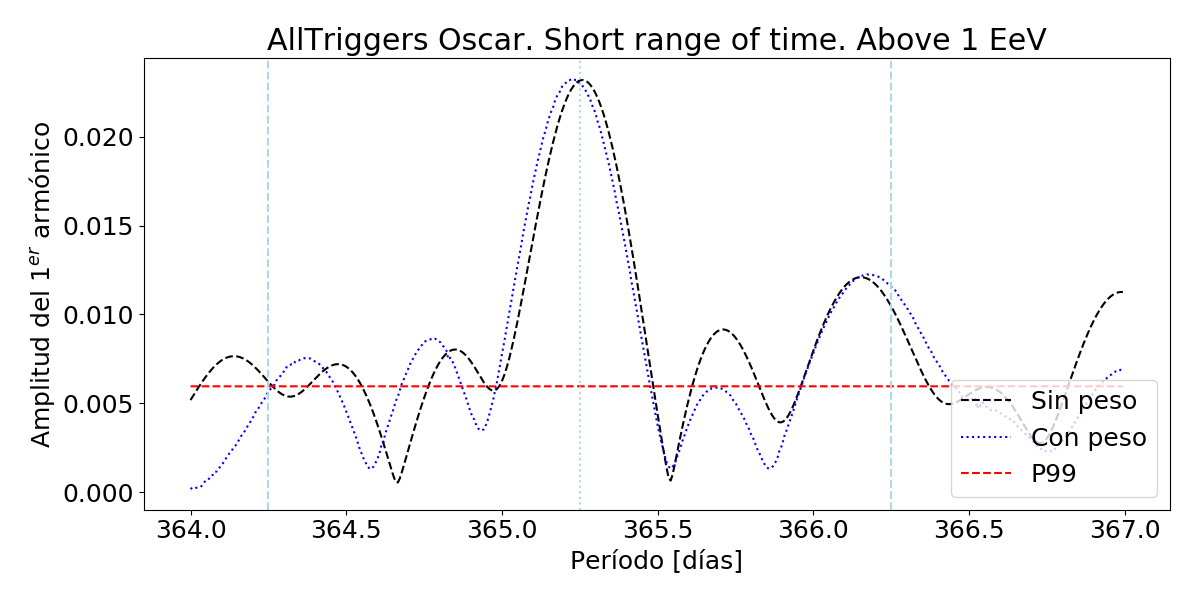
\includegraphics[width=0.6\textwidth]{AllTriggers/AllTriggers_2017_Short_range_Above_1_EeV.png}
				\end{figure}
			En el gráfico de todos los disparos para el archivo de 2017, se ve que hay una modulación anual importante. Es de esperarse ya que la correción del clima aun no fue implementada para este conjuntos de datos.

			Comentario: {\sl Para el análisis en frecuencias, no hace ruido el hecho que la línea del P99 esté tan bajo, siendo que solo depende de la cantidad de eventos, }


% ------> ALL TRIGGERS 2019
		%\subsubsection{Resultados del archivo del 2020}

		%{\bf Esta sección no fue actualizada aún}
		%	\begin{figure}[H]
		%		\centering
		%		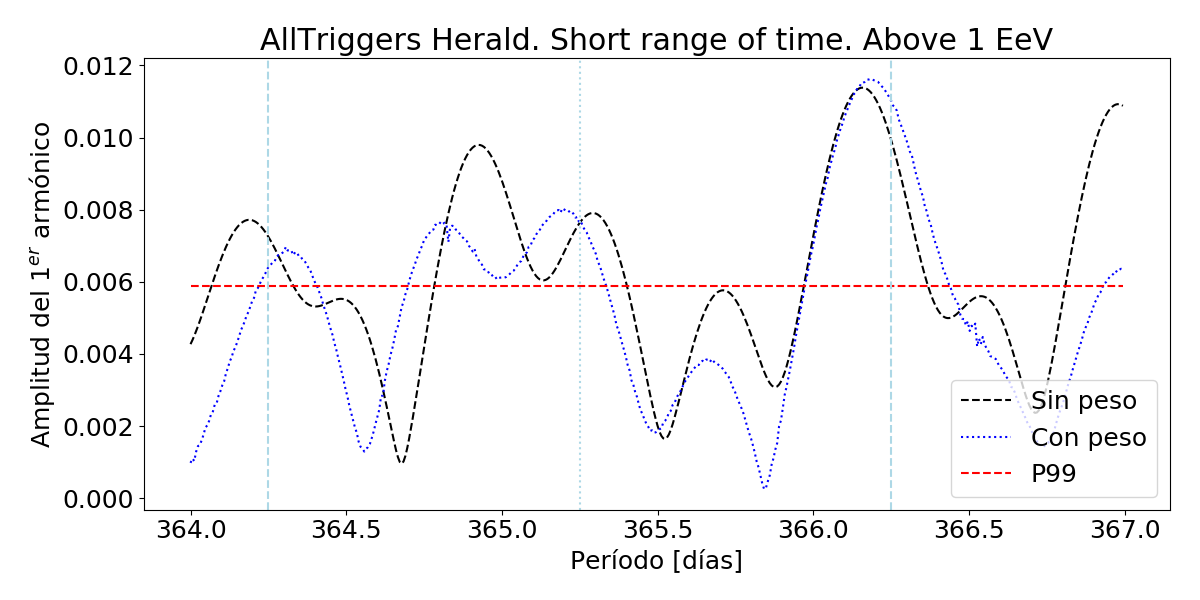
\includegraphics[width=0.95\textwidth]{AllTriggers/AllTriggers_2019_Short_range_Above_1_EeV.png}
		%	\end{figure}

% --> WEATHER STUFF

			\subsubsection{Modulación del clima para todos los triggers}




			Para corroborar los parámetros del clima, primero calculé las tasas de eventos de los archivos del 2017 y 2020 para energías mayores a 1  EeV, donde obtuve los siguientes gráficos Fig.\ref{fig:rate_daily_2017_1EeV} y \ref{fig:rate_daily_2020_1EeV}. 

				\begin{figure}[H]
				
					\begin{subfigure}[b]{0.5\textwidth}
					\centering
					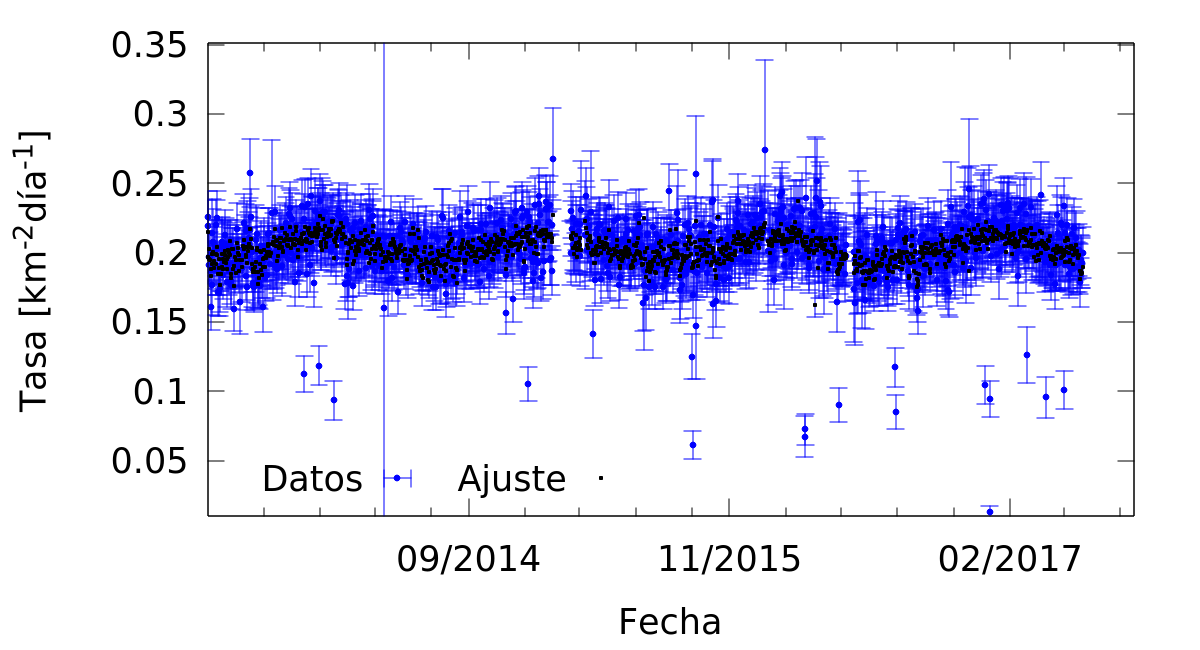
\includegraphics[width=\textwidth]{daily_rate/daily_rate_AllTriggers_2017_1EeV.png}
					\caption{Archivo de 2017} 	\label{fig:rate_daily_2017_1EeV}
					\end{subfigure}%
				\hfill
					\begin{subfigure}[b]{0.5\textwidth}
					\centering
					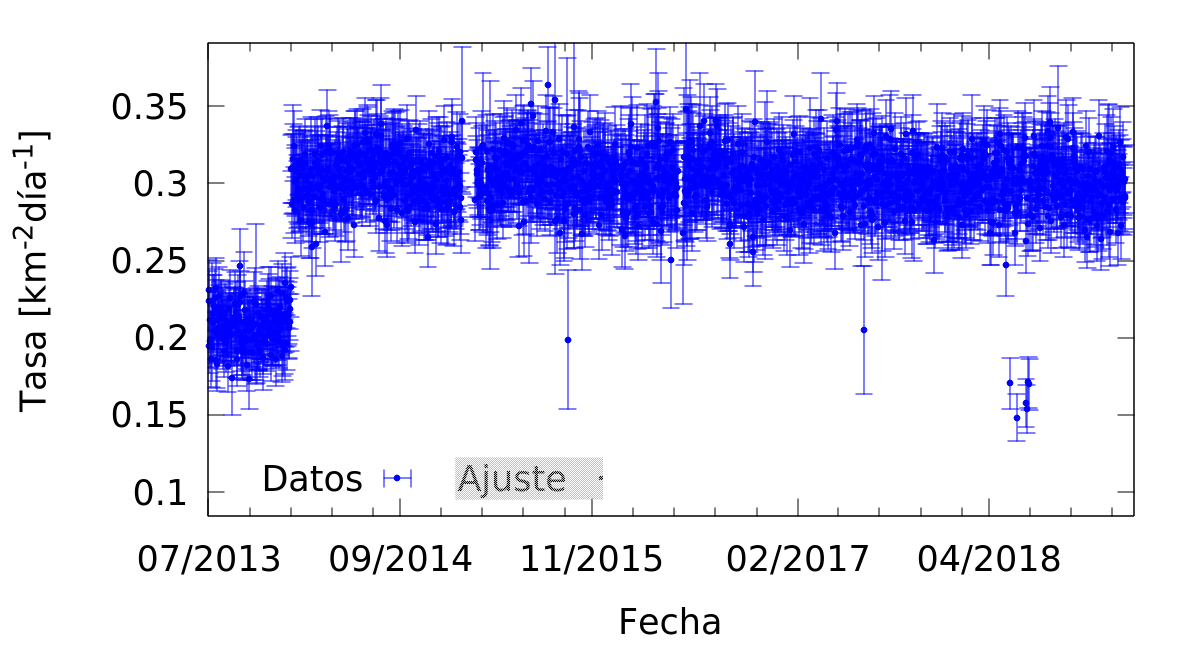
\includegraphics[width=\textwidth]{daily_rate/daily_rate_AllTriggers_2019_1EeV.png}
					\caption{Archivo del 2020} 	\label{fig:rate_daily_2020_1EeV}
					\end{subfigure}
					\caption{Tasa de eventos diaria por encima de 1 EeV para los datos de todos los disparos.}
				\end{figure}

			Después calculé los parámetros del clima para energía mayores a 1 EeV. Para el archivo de 2017 obtuve la Fig.\,\ref{fig:parameters_2017_1EeV}. Los comparé con el paper del weather del main array, para ver si dan algo razonable. Verifiqué las siguientes cosas para el ajuste

			\begin{itemize}
				\item Me fijé que delay en la densidad cada momento fuera de dos  horas
				\item Me fijé que el ajuste no tuviera en cuenta periodos malos, bad periods
				\item Me fijé que el delay de la densidad media también fuera tal que para cada evento estuviera centrada $\pm$12 horas
				\item También me fijé que el rango de tiempo estuviera bien, porque estos datos están disponibles desde el 2013  recién
				\item Me fijé que los $\chi^2$ reducido fuera algo razonable. Todos rondaban alrededor de $1.05$
			\end{itemize}

			EL rango de tiempo que usé fue este: 
			\begin{itemize}
				\item Inicio: 1372680308
				\item Final: 1496275090
			\end{itemize}
				\begin{figure}[H]
					\begin{subfigure}[b]{0.5\textwidth}
					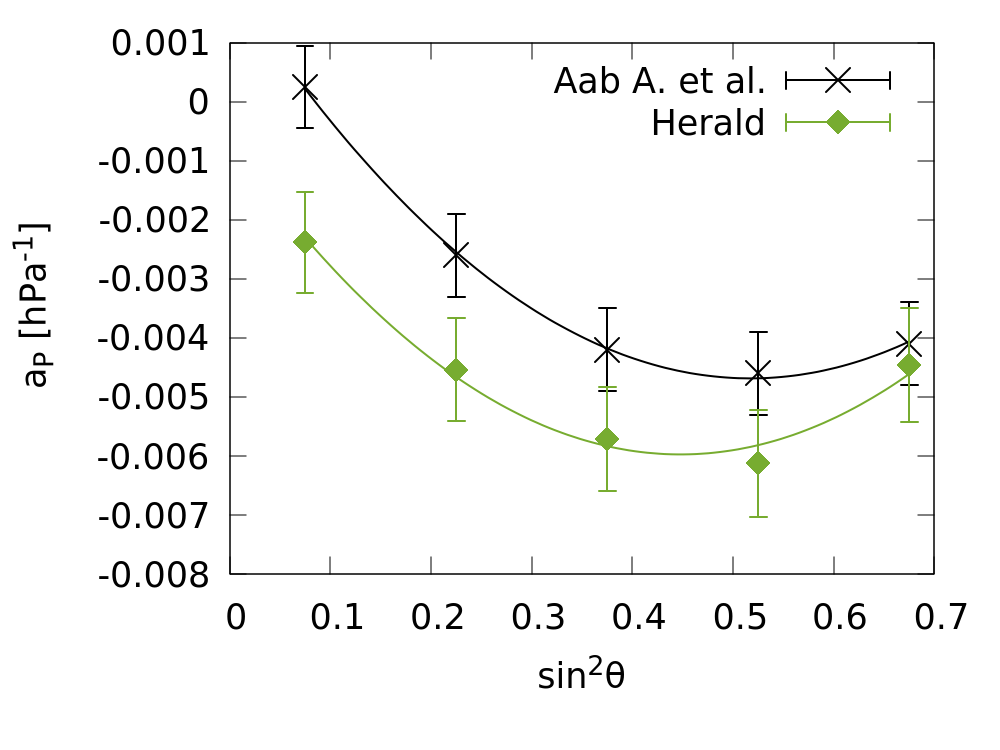
\includegraphics[width=\linewidth]{params/ap_2017_above_1EeV.png}
					\caption{Parámetro $a_P$ }
					\label{fig:ap_2017_1EeV}
					\end{subfigure}%
					\hspace{\fill}
					\begin{subfigure}[b]{0.5\textwidth}
					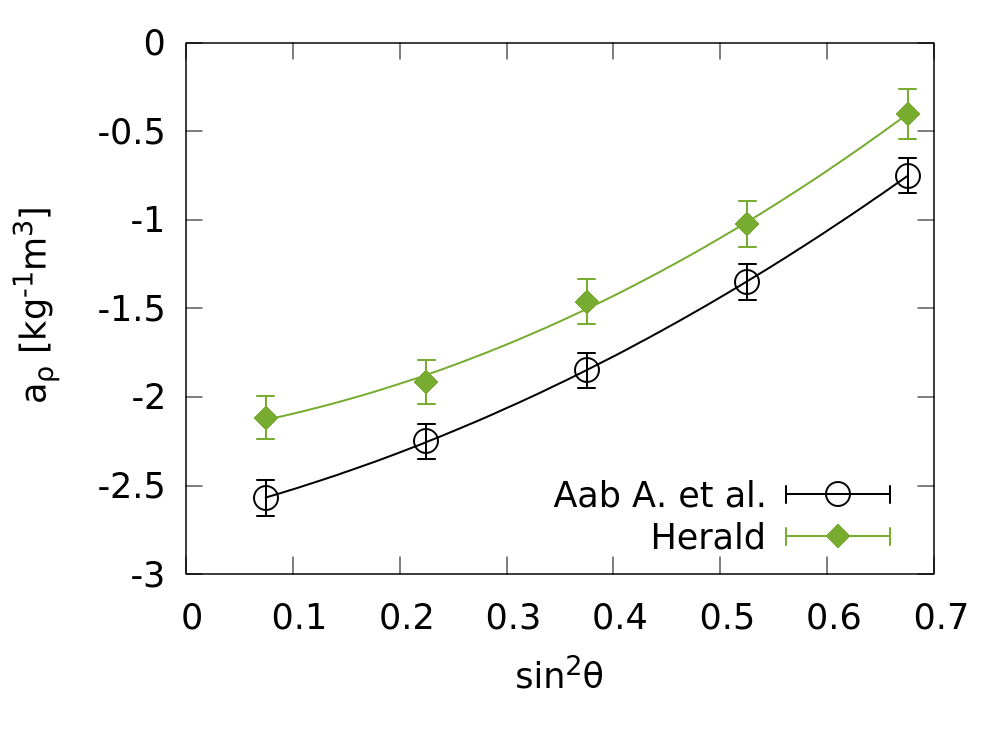
\includegraphics[width=\linewidth]{params/arho_2017_above_1EeV.png}
					\caption{Parámetro $a_{\rho}$ }
					\label{fig:arho_2017_1EeV}
					\end{subfigure}%
					\hspace{\fill}
					\begin{subfigure}[b]{\textwidth}
					\centering
					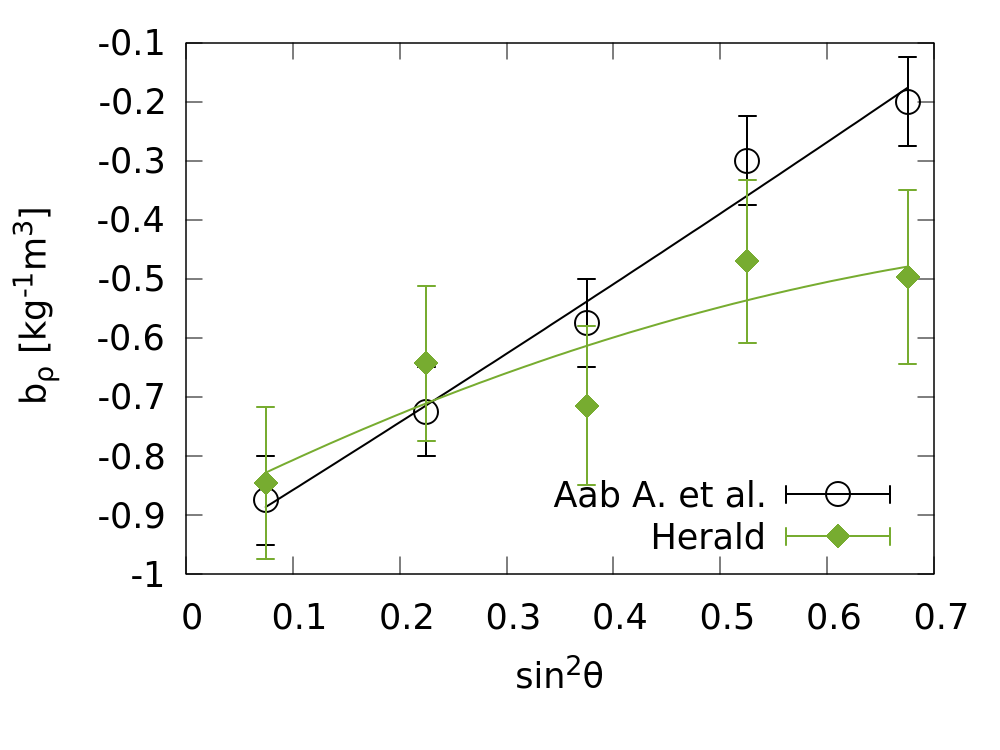
\includegraphics[width=0.5\linewidth]{params/brho_2017_above_1EeV.png}
					\caption{Parámetro  $b_\rho$	 }
					\label{fig:brho_2017_1EeV}
					\end{subfigure}%
					\caption{Parámetros de la modulación del clima considerando los datos para todos los disparos de 2017. Los mismos se comparan con los ajustes obtenidos en \cite{aab2017impact}.}\label{fig:parameters_2017_1EeV}
				\end{figure}

				Lo que más me llama la atención es el comportamiento del parámetro $b_\rho$, que como se discutió en otras oportunidades, tiene que ver con el parámetro $a_\rho$ con una razón de  $1:3$ más o menos. 



			Hacemos el mismo procedimiento con el archivo 2020, {\bf pero filtrando los eventos por el valor de S38 sin corregir por la modulación del clima}. Para calcular la tasa y los parámetros del clima, se toman los eventos después de ese salto de 0.2 a 0.3, obtengo los siguientes resultados:

				\begin{figure}[H]
					\centering
					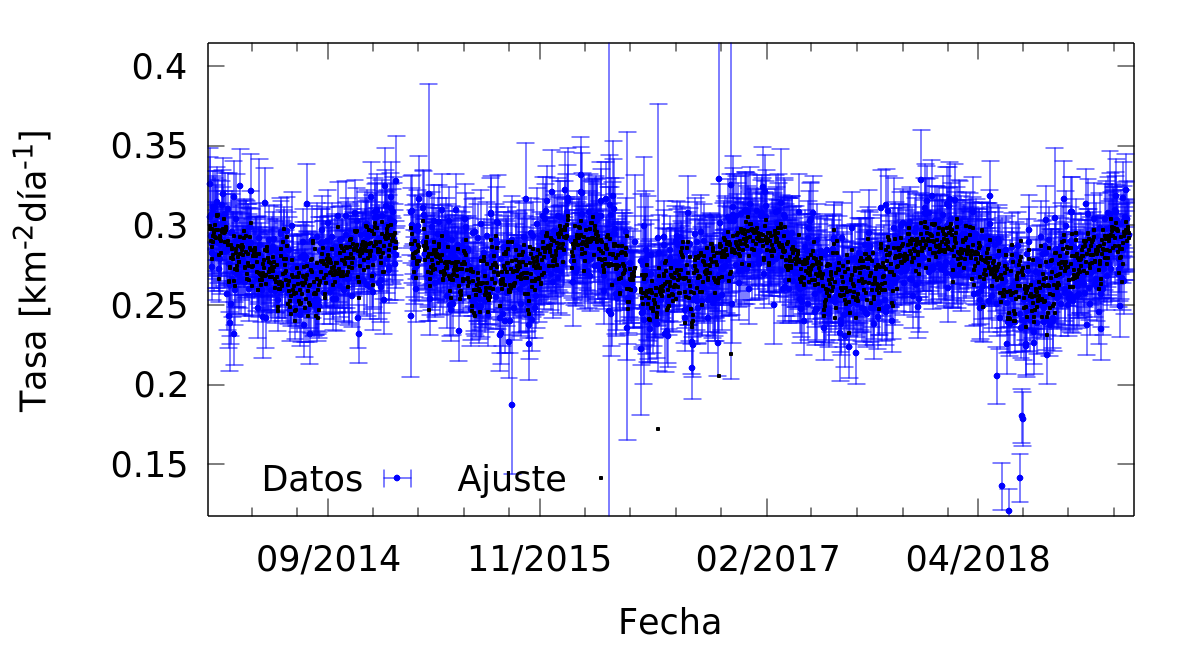
\includegraphics[width=0.5\textwidth]{daily_rate/daily_rate_AllTriggers_2020_1EeV.png}
				\end{figure}

			Acá también verifiqué lo mismo que el caso anterior, lo único que ahora el $\chi^2$ rondaba alrededor de los $1.08$. Siempre verifico que no sea mucho mayor o menor a 1.

			EL rango de tiempo que usé para este caso fue este: 
			\begin{itemize}
				\item Inicio: 1388910508
				\item Final: 1550490858
			\end{itemize}
			
				\begin{figure}[H]
					\begin{subfigure}[b]{0.5\textwidth}
					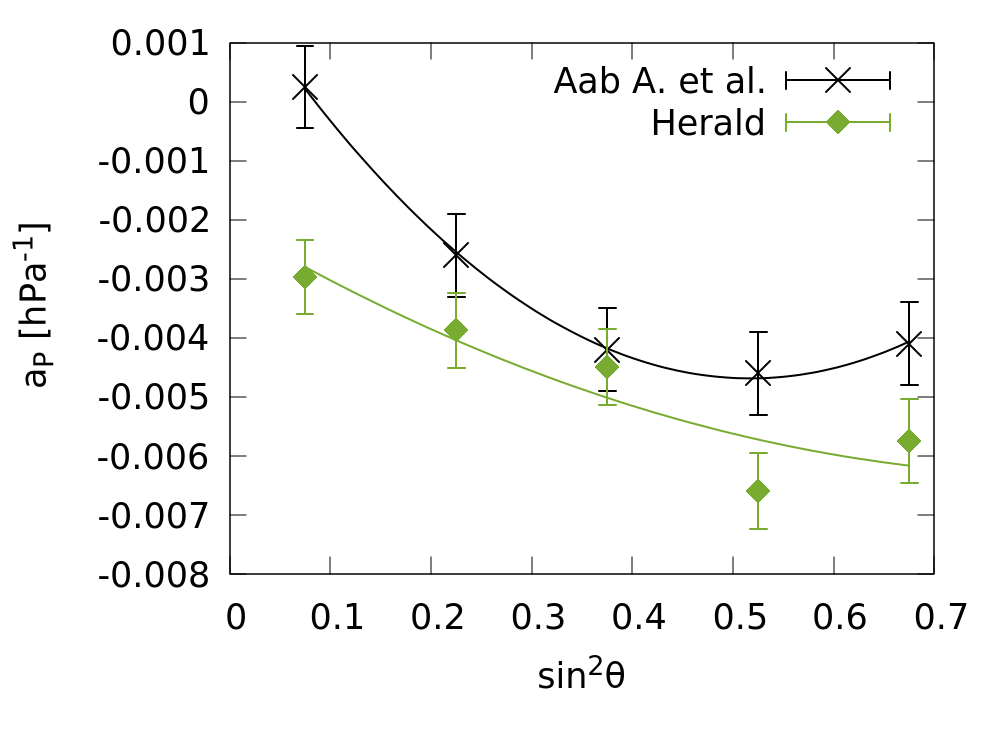
\includegraphics[width=\linewidth]{params/ap_2020_above_1EeV.png}
					\caption{Parámetro $a_P$ }
					\label{fig:ap_2020_1EeV}
					\end{subfigure}%
					\hspace{\fill}
					\begin{subfigure}[b]{0.5\textwidth}
					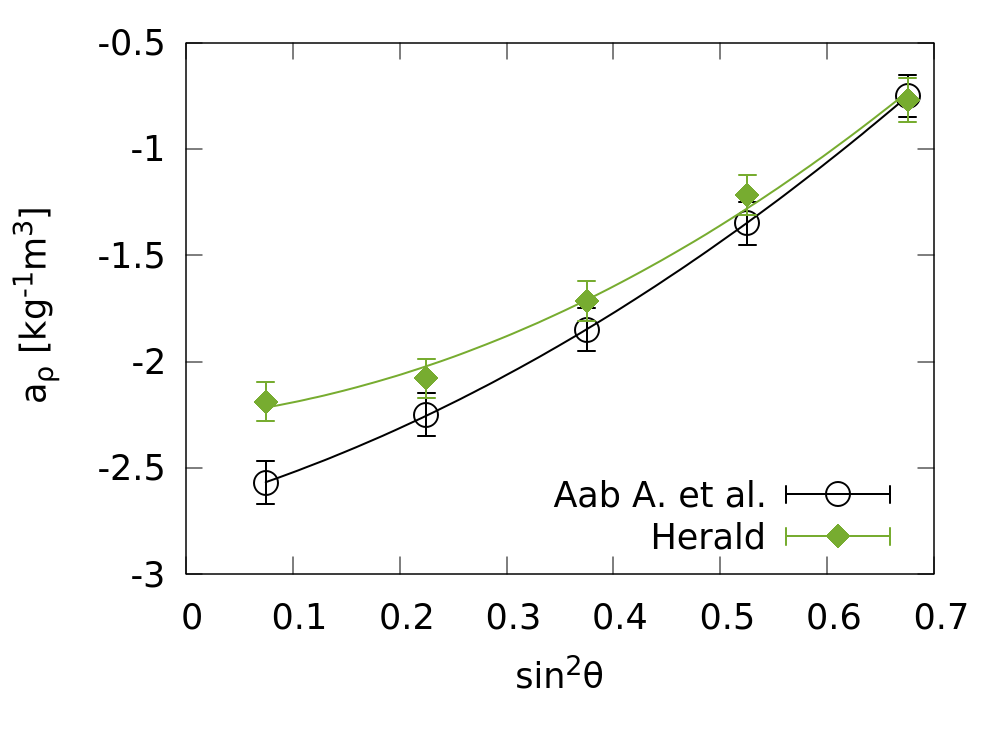
\includegraphics[width=\linewidth]{params/arho_2020_above_1EeV.png}
					\caption{Parámetro $a_{\rho}$ }
					\label{fig:arho_2020_1EeV}
					\end{subfigure}%
					\hspace{\fill}
					\begin{subfigure}[b]{\textwidth}
					\centering
					\includegraphics[width=0.5\linewidth]{params/brho_2020_above_1EeV.png}
					\caption{Parámetro  $b_\rho$	 }
					\label{fig:brho_2020_1EeV}
					\end{subfigure}%
					\caption{Parámetros de la modulación del clima considerando los datos para todos los disparos de 2020. Los mismos se comparan con los ajustes obtenidos en \cite{aab2017impact}.}\label{fig:parameters_2020_1EeV}
				\end{figure}



			Considerando el filtro con el S38 en el archivo 2020 y la energía en el 2017, quiero saber si obtengo parametros  del clima comparables. Ya que el Main Array se corresponden los parametros del 2015 y 2019, yo esperaría que con todos los triggers pase los mismo. Una diferencia importante entre ambos análisis es que los parametros del 2020 contienen eventos hasta el 31/12/2019.


				\begin{figure}[H]
					\begin{subfigure}[b]{0.5\textwidth}
					\includegraphics[width=\linewidth]{params/ap_2017_2020_above_1EeV.png}
					\caption{Parámetro $a_P$ }
					\end{subfigure}%
					\hspace{\fill}
					\begin{subfigure}[b]{0.5\textwidth}
					\includegraphics[width=\linewidth]{params/arho_2017_2020_above_1EeV.png}
					\caption{Parámetro $a_{\rho}$ }
					\end{subfigure}%
					\hspace{\fill}
					\begin{subfigure}[b]{\textwidth}
					\centering
					\includegraphics[width=0.5\linewidth]{params/brho_2017_2020_above_1EeV.png}
					\caption{Parámetro  $b_\rho$	 }
					\end{subfigure}%
					\caption{Parámetros de la modulación del clima considerando los datos para todos los disparos del archivo 2017 y 2020. Los mismos se comparan con los ajustes obtenidos en \cite{aab2017impact}.}
				\end{figure}

			Se ve que estos parametros no son comparables. 

{\bf Hasta acá está verificado}


\subsubsection*{To do list }
		\begin{itemize}
			\done (DONE) ¿estoy haciendo bien la cuenta? 
			\done (DONE) el log en ln o log10 para cpp? es ln==log en cpp
			\done¿Hay algo en la aproximación de rayleigh que se pasó por alto? Sigo buscando
			\done (DONE?) ¿Entiendo bien la approx? --Creo que sí, leí el paper que referencian, pero puede que un detalle se me halla escapado
	\item Hacer 4-8 EeV
	\done Comparar con ICRC por debajo de full efficency (¿necesario?): {\sl No, no es necesario}
	\done Entender que está pasando con el percentil 99 : {\sl Se discutió con Mollerach}
	\done {\sl (DONE)} Actualizar los gráficos para long range 
	\done {\sl (DONE sort of)} Verificar el weather de AllTriggers2017 por encima de 1 EeV
	\item Empezar el código para analizar más momentos (dipole, quadruplo): {\sl work in progress}
	\done {\sl (DONE)} Mandar mail
	\done Actualizar los rango de tiempo del ICRC 2019 y el AllTriggers 2019
\end{itemize}



\subsubsection*{How to do the analisis right?}

\begin{itemize}
	\done Fijate que el rango de tiempo esté bien
	\done Asegurate que los archivos esten actualizados a la fecha que queres analizar.
	\done Fijarse si tengo que usar 5t5 o 6t5
\end{itemize}

\subsubsection*{Comentarios importantes}

\begin{itemize}
	\item Para el rango de energía 2 EeV para arriba usamos el  Main\_Array, porque ya es más o menos full eficiency
	\item En el bin de energía entre 1\,EeV y 2\,EeV usamos el archivo AllTriggers
	\item Tengo ambos archivos hasta el 31 12 2019, así también como el archivo del clima actualizado hasta  Monday, 18 February 2019 23:55:00
\end{itemize}



{\bf 1395680272} CHECK THIS EVENT!!!!!!!!!!!

	
%\begin{enumerate}
	%\item ¿Hizo alguna diferencia a la energía la corrección del clima?
	%\item ¿Hizo alguna diferencia la evolución del tiempo de los hexágonos a los parámetros del clima?
	%\item  ¿Disminuyó la modulación?
	%\item ¿El S38 sin corregir por clima me da los mismos resultados que lo anterior?
%	\item 
%\end{enumerate}


En este trabajo se analizaron los efectos de las variaciones de los parámetros del clima sobre el desarrollo en la atmósfera de las lluvias atmósferas. Se analizaron datos del arreglo de detectores espaciados 1500 m entre sí del Observatorio Pierre Auger, en el periodo 2005-2015 y 2005-2018 extendiendo los periodos de tiempo estudiados anteriormente. Se emuló los resultados de la corrección de la modulación del clima sobre el periodo 2005-2015 de la colaboración Pierre Auger, obteniéndose resultados compatibles. Se observó que posterior a la corrección, la modulación del clima se vio disminuida. Para eventos con energía mayor a $2\,$EeV, esta modulación es despreciable.

Posterior a los análisis anteriores, se estudió la modulación del clima mediante el valor del $S_{38}$ sin la corrección propuesta por trabajos anteriores. Se observó que los parámetros del clima obtenidos de estos datos son compatibles con los utilizados en la reconstrucción oficial. Se realizó un corrección a  la energía mediante los coeficientes nuevos, observándose que la modulación era despreciable para energías mayores a $2\,$EeV. 


%En este trabajo se estudió eventos con energía mayor a $1\,$EeV entre los años 2005-2018, extendiendo los periodos de tiempo estudiados anteriormente.



\chapter{Introducción}
	\graphicspath{{../0_Introduccion/}}
	% INTRODUCCION

La parte superior de la atmósfera terrestre está siendo constantemente bombardeada con partículas provenientes del espacio, con energías de los $10^{10}\,$eV para arriba. Estas partículas son conocidas como rayos cósmicos (RC) y han sido medidas desde los años 60s \cite{linsley1961extremely}. Aunque el área lleva tiempo siendo estudiada, los mecanismos que producen los RCs y las zonas del espacio donde se originan los mismos siguen siendo investigadas por distintos experimentos. 


Por encima de una energía de $10^{14}\,$eV, los RCs que llegan a la atmósfera pueden interactuar con las moléculas de la misma,  y así producir cascadas de partículas secundarias. Dependiendo de la energía del primario, es decir el RC que generó la lluvia, estas partículas pueden ser medidas usando detectores sobre la superficie de la Tierra. Esta cascada es conocida como lluvia atmosférica extendida o \emph{EAS} y está compuesta por una componente electromagnética, que consiste en electrones, positrones y fotones, y una componente muónica. Las partículas secundarias cargadas también pueden excitar moléculas de nitrógeno en el aire que producen fotones de fluorescencia y pueden ser observados por telescopios durante noches claras.


El observatorio Pierre Auger está ubicado en la ciudad de Malargüe, provincia de Mendoza. El mismo fue construido para detectar las partículas secundarias de las EASs producidas por RCs, con energía por encima de $0.1\,$EeV. La adquisición de datos empezó en el año 2004. El observatorio posee un sistema híbrido de detección, ya que combina un arreglo de detectores de partículas sobre la superficie y un conjunto de telescopios que detectan los fotones de fluorescencia. Cuando el observatorio  registra una EAS que llega a la superficie y reconstruye la dirección de llegada del RC, se dice que se ha detectado un \textit{evento}.


Los análisis presentados en este trabajo fueron realizados con los eventos obtenidos por $\sim 1600$ detectores Cherenkov, dispuestos sobre de $\sim 3000\,\text{km}^2$ a  $1500\,$m entre sí. Un conjunto de 7 detectores adyacentes, es decir una en el medio y 6 en los lados, forman una celda hexagonal. Esta disposición de tanques se menciona como \textit{arreglo principal}.   Cada detector consiste en un tanque cilíndrico con 12 toneladas de agua ultra-pura de $1.2\,$m de alto. En la parte superior del tanque están instalados 3 foto-multiplicadores que monitorean la radiación Cherenkov en el agua. El conjunto del tanque y la electrónica de detección  se menciona durante este trabajo como \textit{Surface Detector} o \textit{SD}.  Cada detector está midiendo constantemente los fotones en el agua. Muchos de estos fotones son producidos por ruido y otros por partículas secundarias de una EAS. Los SDs cuentan con algoritmos o reglas para discernir ruido de un evento causado por un rayo cósmico, estos son los algoritmos de disparo.


\section{Acerca de todos los disparos del SD}

A medida que los tanques pasan más tiempo midiendo, también van perdiendo sensibilidad a los eventos de bajas energías. Esto es una desventaja del disparo estándar en los SDs en el rango $1\,$EeV - $2\,$EeV, ya que la eficiencia completa  del disparo estándar se obtiene para eventos de energía mayor a $2.5\,$EeV.  En la Fig.\ref{fig:futuro}, para los datos presentados en el ICRC 2019, se observa como la energía media de los eventos para distintos rangos de tiempo va aumentando, además que la proporción de eventos por debajo de $3\,$ EeV disminuye. 

\begin{figure}[H]
	\centering
	\includegraphics[width=0.8\textwidth]{histograma_evolucion_eventos.png}
	\caption{Histograma de eventos  del Disparo Estándar por rango de tiempo medido por el Observatorio Pierre Auger}
	\label{fig:futuro}
\end{figure}

\begin{figure}[H]
	\centering
	\includegraphics[width=0.8\textwidth]{figura_harari.png}
	\caption{Histograma de eventos de  Todos Los Disparos por rango de tiempo medido por el Observatorio Pierre Auger}
	\label{fig:TLD}
\end{figure}


El análisis del trabajo de licenciatura fue realizado sobre los eventos medidos utilizando el disparo estándar del arreglo principal, cuya eficiencia varía con la energía del CR. Para el disparo estándar, los eventos con energía mayor a $3\,$EeV y ángulo cenital $\theta<60^o$ o  por encima de $4\,$EeV y $\theta<80^o$, son detectados con una eficiencia del 100\%. Por lo tanto, el análisis en el rango de energía entre $1\,$EeV - $2\,$EeV requiere factores relacionados con la eficiencia del disparo en función de la energía. Estos factores son obtenidos de manera fenomenológica \cite{taborda}. 

Para superar esta dificultad y  poder recuperar la sensibilidad para bajas energías, a partir del año 2013  se implementó otros algoritmos de disparo en los SDs, llamados ToTd y MoPS \cite{pierre2013plans}. Estos algoritmos de disparo se mencionan en este trabajo como \textit{todos los disparos}. 

La implementación de los ToTd y MoPS fue llevada a cabo mediante una actualización de la electrónica de los SDs para bajar el umbral de disparo, en particular para las señales de la componente electromagnética de la EAS, mejorando así la reconstrucción de eventos mediante la separación fotón/hadrón para bajas energías  \cite{pierre2013plans}. Con esta mejora, el umbral de eficiencia completa para todos los disparos es menor que el disparo estándar, este umbral es de una energía de $1\,$EeV. En la Fig\,\ref{fig:triggers} se comparan las eficiencia del disparo estándar y todos los disparos en función de la energía del evento. De tal manera que, al estudiar los eventos en el rango $1\,$EeV - $2\,$EeV,  no son necesarios los factores de eficiencia y sólo pueden afectar los cambios de la exposición direccional del observatorio.


\begin{figure}[H]
  \centering
  \includegraphics[width=0.75\textwidth]{comparacion_triggers.png}
  \caption{La eficiencia del disparo en función de la energía para eventos con ángulo cenital $\theta$ menor a $60^o$. Este figura fue extraída del trabajo \cite{triggers_ref}}
  \label{fig:triggers}
\end{figure}


Una desventaja de todos los disparos sobre el disparo estándar, es que el último tiene una mayor cantidad de años medidos, ya que se adquieren datos  desde el año 2004 con este algoritmo. Esto es conveniente ya que mientras más años han sido medidos es más factible que los efectos espúreos se cancelen. En cambio, para todos los disparos, el análisis  es posible desde el año 2013. Entre inicios del 2004 y finales del 2019, el conjunto de eventos del disparo estándar tiene $6\,975\,194$ eventos sin clasificar, es decir todos los eventos registrados por el observatorio sin discriminar por energía. En cambio entre mediados del 2013 hasta fines del 2019, el archivo de eventos para todos los disparos tiene $13\,739\,351$ eventos sin clasificar, por lo que el menor tiempo de medición se compensa con la eficiencia del disparo.


\section{Acerca de los eventos} \label{filtro}

Se aplican cortes a los eventos para asegurar la eficiencia completa de los detectores. Estos cortes implican límites en ángulo cenital $\theta$ de los eventos, en la cantidad de vecinos al tanque de mayor señal, además de restringirse a eventos medidos en condiciones normales, es decir, cuando los sistemas de comunicación del Observatorio funcionan sin inconvenientes. De esta manera, podemos prescindir de otros factores de corrección.

A partir de los registros de eventos del arreglo principal con todos los disparos, se consideran solamente los eventos que cumplan las siguientes características:

    \begin{enumerate}
      \item La calidad de la reconstrucción depende de la energía y del ángulo cenital $\theta$ del evento.  Para el disparo estándar los eventos por debajo de los $4\,$EeV, se consideran los eventos con $\theta < 60^o$, en cambio para eventos por encima de esta energía se consideran hasta $\theta < 80^o$. Para todos los disparos se consideran solo los eventos con $\theta<60^o$.
      \item Los datos del evento son recopilados sin inconvenientes. Este filtro se conoce como \emph{Bad period flag} o $ib$. Un valor de 1 indica un buen periodo. Con este filtro se descartan eventos debido a probables fallas de alimentación o problemas de comunicación o adquisición que podrían inducir errores en el análisis.
      \item Buena reconstrucción de la lluvia atmosférica asociada al evento.
      \item El tanque de mayor señal está en el interior de un hexágono de tanques activos. Estos eventos se conocen como \textit{eventos 6T5}.
    \end{enumerate}


\subsection{Acerca del registro de hexágonos}\label{hexagonos_rate}

La cantidad de celdas  activas sobre el observatorio está relacionado con el filtro de eventos $6T5$, que garantiza la calidad de la reconstrucción del evento. El observatorio lleva un registro de la cantidad de hexágonos activos cada 5 min, además de registrar las condiciones atmosféricas en distintas estaciones de clima sobre la superficie del observatorio. 


\section{Acerca de la tesis de licenciatura}

Durante la tesis de licenciatura se analizaron los efectos de las condiciones atmosféricas durante el desarrollo de las EAS.  Se analizaron los datos adquiridos durante en el periodo 2005-2018 por el arreglo principal. De esta manera, se extendió los periodos estudiados anteriormente en los siguientes trabajos \cite{abraham2009atmospheric}, \cite{abreu2012description}   y \cite{aab2017impact}. 

Los efectos atmosféricos afectan principalmente a la atenuación de la componente electromagnética  de la EAS, en particular depende fuertemente de la temperatura y presión. Estos efectos  se caracterizan por parámetros dependientes del ángulo cenital del evento y por la presión, densidad y temperatura al momento de su detección. Los parámetros mencionados se utilizan para corregir las señales registradas por los SDs. Las correcciones del clima utilizadas por la colaboración Pierre Auger fueron implementadas a partir del trabajo \cite{aab2017impact} en el 2017. 

Durante el trabajo de la licenciatura se reprodujo el análisis de la modulación del clima sobre el periodo 2005-2015 del trabajo \cite{aab2017impact}, obteniéndose resultados compatibles. También se estudió la modulación del clima mediante el valor de la señal medida por los SDs, $S_{38}$, sin la corrección propuesta por \cite{aab2017impact}, además de extender el rango de tiempo analizado hasta el 2018. Se observó que los parámetros del clima obtenidos en este análisis sobre  $S_{38}$  son compatibles con los utilizados en la reconstrucción oficial. 
	
	
\chapter{Métodos}
	\graphicspath{{../1_Metodo/}}
	% METODOS
El estudio de la distribución de las direcciones de arribo de los eventos es una herramienta importante para obtener información sobre el origen de los RCs . Las irregularidades sobre el flujo casi isotrópico de los RCs, en un rango de energía, pueden deberse a  zonas del espacio donde se producen más RCs que en otras, estas irregularidades se conocen como anisotropías. 

El análisis de anisotropías a grandes escalas angulares suele ser hecho sobre las irregularidades de la distribución de eventos en ascensión recta $\alpha$, ya que el arreglo principal tiene una exposición direccional en función de esta coordenada casi constante \cite{referencia_anis}.

\section{Cálculo de los coeficientes de Fourier para el análisis de anisotropía en ascensión recta}

Las anisotropías son variaciones pequeñas por lo que eliminar todo factor espurio en el análisis es importante. Para obtener la amplitud de la misma en ascensión recta, se estudia la frecuencia sidérea ($f_{sid}=366.25\,$ ciclos/año) \cite{taborda}. Los errores sistemáticos debido a la modulación de eventos por el clima u otros errores propios de la adquisición de datos, aparecen en la frecuencia solar  ($f_{sid}=365.25\,$ ciclos/año), por lo que se debe tener en consideración el análisis de esta frecuencia. La frecuencia anti-sidérea ($f_a=364.25\,$ ciclos/año) es una frecuencia que puede indicar efectos sistemáticos en la amplitud de la anisotropía en la frecuencia sidérea \cite{farley1954sidereal}. La mezcla entre modulaciones diarias y anuales induce bandas laterales ubicadas a $\pm1\,$ciclo/año con respecto a la solar \cite{taborda}. Por estos motivos se toman estas frecuencias  como referencia.

  \subsection{Variaciones relativas de los hexágonos} \label{peso_hexagonos}

Para corregir las variaciones de la exposición del observatorio, podemos definir un peso  $w_i$ por cada evento $i$, que corrige la variación  $\Delta N_{cell}(\alpha^0)$ en función de la ascensión recta del cenit del observatorio $\alpha^0$ durante el rango de tiempo estudiado. Estas variaciones pueden deberse al crecimiento del arreglo a través de los años,  por caídas en la comunicación del observatorio con los SDs u otros motivos. 

El factor $\Delta N _{cell}(\alpha^0)$ tiene en cuenta que la exposición  direccional  el observatorio no es uniforme en tiempo sidéreo.  Se obtiene sumando el número de celdas durante el periodo de medición, en cada segmento de $\alpha^0$ y luego se normaliza con el valor medio de los segmentos.

Para calcular estos pesos $w_i$, se sigue el algoritmo presentado a continuación:
     
      \begin{enumerate}
        \item Se establecen una frecuencia $f$  y un rango de tiempo a estudiar. Por ejemplo, se desea estudiar la frecuencia solar entre el 1 de Enero del 2014 a las 12:00:00 GMT y el 1 de Enero del 2020 a las 12:00:00 GMT.

        \item Cada dato del registro de hexágonos, tomado en un momento $t$ durante el rango seleccionado, se clasifica según la cantidad de horas desde un momento de referencia $t_0$. Esta referencia $t_0$ se tomará como el 1 de Enero del 2005 a las 00:00:00 GMT, o  $21\,$hs del 31 de Diciembre del 2004, según la hora local de Malargüe.

        \item Podemos asociar una coordenada angular $h$ a $t$  y $f$  utilizando la siguiente expresión:
         \begin{equation}
          h = (t-t_0) \times \frac{360^o}{24\text{hs}} \times\frac{f}{f_{Solar}} + h_0
          \label{eq:h_horas} 
        \end{equation}
        El factor $\nicefrac{f}{f_{Solar}}$ sirve para hacer un cambio de escala temporal entre los periodos de distintas frecuencias. Se usa como referencia la $f_{Solar}$ dado que las horas (solares) se basan en esta frecuencia, y el valor de $h_0=31.4971^o$ representa la ascensión recta del cenit del observatorio en el momento utilizado como referencia.
        
        \item  Para simplificar el cálculo del peso de los hexágonos, se divide los $360^o$ de la ascensión recta en $L$ segmentos de $\nicefrac{360}{L} ^o$ cada uno. Para clasificar un dato se  toma  el valor $h$  y se calcula
        \begin{equation}
          h' = h\, mod \,360 %=  h - 360\Big \lfloor \frac{h}{360} \Big \rfloor
          \label{eq:h_primado}
        \end{equation}
        donde la función $mod$ representa la función módulo que devuelve un número real positivo. Con el valor de $h'$ del dato, se asigna el mismo al segmento $k$ que le corresponde, mediante la siguiente expresión
        \begin{equation}
          k = \bigg \lceil \frac{h'}{360}\times L \bigg \rceil
        \end{equation}
        donde $\lceil a \rceil$ representa la función techo \footnote{La función techo da como resultado el número entero más próximo por exceso}. Por ejemplo, si optamos por $L=24$ y un dato en particular resulta con  $h=395\,^o$, esto implica que $h'= 35^o$ y que $k=\lceil 2.333 \rceil=3$, por lo tanto, este registro corresponde al segmento en la $3^{a}$ posición.

        \item Una vez clasificados todos los datos del registro de hexágonos, se calcula la suma  $N_{hex, j}$ de los datos que cayeron un segmento $j$ dado. Para definir la variación relativa de hexágonos  $\Delta N_{cell,k}$ de un segmento $k$ en particular, necesitamos la media de hexágonos por segmento $ \langle N \rangle$  para normalizar las variaciones.
       \begin{align}
         \langle N \rangle &= \sum^{L}_{i=1} \frac{N_{cell, i}}{L}  \qquad
         \Delta N_{cell,k} = \frac{N_{cell, k}}{\langle N \rangle}  \label{epepe}
       \end{align}

      \end{enumerate}
 En la Fig.\ref{fig:pesos_referencia} se muestran las variaciones relativas de los hexágonos en función de la ascensión recta del cenit del observatorio para las frecuencias mencionadas. Este análisis fue realizado en el marco del trabajo \cite{referencia_pesos} con eventos del periodo 2004-2017. 



       En la Fig.\ref{fig:pesos_ejemplo} se observan los valores obtenidos de $\Delta N_{cell,k}$  con el código escrito para este trabajo, en función de la ascensión recta del cenit  para $L=288$ segmentos. Se analizó el conjunto de datos  utilizado para obtener los resultados la Fig.\ref{fig:pesos_referencia}, con el fin de validar dicho código. Los datos se analizaron desde el 1 de Enero del 2004 a las 00:00:00 GMT  hasta el 1 de Enero del 2017 a las 00:00:00 GMT. Se  observa que estos los resultados obtenidos son compatibles con la Fig.\ref{fig:pesos_referencia}
      
      \begin{figure}[H]
          \centering
              \includegraphics[width=0.5\linewidth]{pesos_referencia.png}  
              \caption{Valores de $\Delta N_{cell, k}$ en el rango 2004-2017 para distintas frecuencias obtenidas en el trabajo \cite{referencia_pesos}.}
              \label{fig:pesos_referencia}
        \end{figure}

       \begin{figure}[H]
          \centering
              \includegraphics[width=0.75\linewidth]{weigths_2020.png}
              \caption{Valores de $\Delta N_{cell, k}$ en el rango 2004-2017 para distintas frecuencias utilizando el código escrito en este trabajo.}
              \label{fig:pesos_ejemplo}
        \end{figure}

    Para una representación fiel entre los registros de los hexágonos y los pesos de los eventos, se optó por clasificar los datos de los hexágonos en $288$ segmentos, donde cada segmento tiene un ancho de $1.25^o$. Esto es conveniente ya que la actualización del registro de hexágonos se realiza una vez  cada $5\,$min como se menciona en la sección \ref{hexagonos_rate}. Esta tasa de actualización es equivalente a decir que la adquisición se realiza cada vez que el cenit del observatorio barre  $1.25^o$ en ascensión recta sobre la esfera celeste.


  \subsection{Cálculo de Rayleigh en ascensión recta para una frecuencia dada} \label{rayleigh}

  Un procedimiento para estudiar anisotropías en la direcciones de arribos de los RCs es realizar un análisis de Fourier en ascensión recta $\alpha$. La distribución en ascensión recta $\alpha$ del flujo de RCs $I(\alpha)$ que llega al arreglo principal puede caracterizarse por las amplitudes $r_k$ y fases $\phi_k$ de su expansión en serie de Fourier al $k-$ésimo orden. 

  \begin{equation}
    I(\alpha) = I_0 \bigg ( 1+ \sum^\infty_{k=1} r_k\cos{[k(\alpha - \phi_k)]} \bigg) = I_0 \bigg ( 1+ \sum^\infty_{k=1} a_k\cos{k\alpha} +  b_k\sin{k\alpha} \bigg ) 
  \end{equation}
  donde $a_k=r_k\cos k\phi_k$ y $b_k=r_k\sin k \phi_k$, y $I_0$ es el flujo medio. La distribución $I(\alpha)$ puede obtenerse a partir de la distribución de direcciones de arribo de los eventos observados.  En este trabajo, suponiendo que existieron $N$ eventos en el rango analizado, se considera que los mismos tienen una distribución en ascensión recta del tipo $\nicefrac{dN}{d\alpha}= \sum^N_{i=1} \delta(\alpha - \alpha_i)$ \cite{taborda}. 

  Como se mencionó anteriormente, los análisis en ascensión recta están asociados a la frecuencia sidérea. Para realizar el análisis de los eventos en cualquier frecuencia arbitraria, es necesario modificar $\alpha$ por $\tilde{\alpha}$. Esta nueva variable tiene la forma como se utiliza en el trabajo \cite{taborda}:
  \begin{equation}
    \tilde{\alpha} = 2\pi f_x t_i + \alpha_i - \alpha_i^0(t_i) \label{ra_mod}
  \end{equation}
  donde $f_x$ es el frecuencia arbitraria a estudiar, $t_i$ es el momento en que ocurrió el evento y $\alpha_i^0(t_i)$ es la ascensión recta del cenit del observatorio en el momento del evento. Si la frecuencia a analizar es la sidérea, el análisis con $\alpha$ y $\tilde{\alpha}$ arrojan los mismos parámetros $r_k$ y $\phi_k$.

 Clasificando a los eventos mencionados en la sección \ref{specs} según el valor de la ascensión recta y considerando que todos los eventos tienen un peso uniforme de $w_i=1$, se dicen que los eventos fueron analizados \textit{sin pesos}, donde no consideramos la corrección de la exposición. En caso contrario, se habla de análisis \textit{con pesos} de los hexágonos  y estos pesos se calculan como se menciona en la sección anterior.

  Para realizar el análisis de frecuencias de los eventos, en el $k$-ésimo orden en la expansión de Fourier, se siguen los siguientes pasos.

        \begin{enumerate}
        \item Fijando un rango de tiempo y un rango de energía en el cual se desea estudiar la anisotropía, se establece una frecuencia en particular $f$ a analizar. Siguiendo el ejemplo de la sección anterior, se analiza la frecuencia solar entre el 1 de Enero del 2014 a las 12:00:00 GMT y 2019 hasta el 1 de Enero del 2020 a las 12:00:00 GMT.

        \item Con los eventos ya filtrados según el criterio de la sección \ref{filtro}, asigno cada evento $i$ un valor $h_i$, definida en la Ec.\ref{eq:h_horas}

        \item En caso de considerar los pesos de los hexágonos, para asignar el peso correspondiente al evento, se asocia a un segmento $k$, calculado en la sección \ref{peso_hexagonos}, mediante el valor de $h'_i$ definido en la Ec.\,\ref{eq:h_primado}. Luego, el peso asignado $w_i$  al evento $i$ es: $ w_{i}= (\Delta N_{cell,k})^{-1}$, caso contrario, se toman que todos los eventos tiene $w_i=1$.
        
        \item Para el análisis en frecuencias, a partir del valor de $h_i$ se asigna el ángulo $\tilde{\alpha}_i$ definida en la Ec.\ref{ra_mod}. La implementación en el código es de la siguiente manera: 
        \begin{equation}
         \tilde{\alpha}_i = 2\pi \frac{h_i}{24} + \alpha_i -\alpha^0_{i}
        \end{equation}
        donde $\alpha_i$  representa la ascensión recta del evento y $\alpha^0_{,i}$ la ascensión recta en el cenit del observatorio en el momento del evento. Cabe resaltar que la información de la frecuencia que se está estudiando se encuentra en el valor de $h$. Si la frecuencia a estudiar fuera la sidérea, el término $2\pi \frac{h}{24} $ seguiría el cenit del observatorio, por lo que este término sería equivalente a $\alpha^0_{i}$, por lo tanto en esta frecuencia $ \tilde{\alpha}_i =\alpha_i$ como es de esperarse. 
        
        \item Para calcular los coeficientes de Fourier del k-ésimo armónico $a_k$ y $b_k$, se siguen los siguiente pasos:
        \begin{enumerate}
          \item Por cada evento  $i$ se calculan los siguientes valores:
          \begin{equation}
             a_{ik}' = {w_i}\cos k\tilde{\alpha}_i \qquad
             b_{ik}' = {w_i}\sin k\tilde{\alpha}_i
         \end{equation}
         \item Una vez que se obtuvieron los valores de $a_{ik}'$ y $b_{ik}'$ para todos los eventos en el rango de tiempo estudiado, se calculan los coeficientes definidos en el trabajo \cite{analisis_fourier} mediante:
         \begin{alignat}{3}
          \mathcal{N} &= \sum^{Eventos}_i w_i \qquad
            a_k = \frac{2}{\mathcal{N}} \sum^{Eventos}_i a_{ik}' \qquad
            b_k = \frac{2}{\mathcal{N}} \sum^{Eventos}_i b_{ik}'  
         \end{alignat}
        \end{enumerate}
        \item Con los coeficientes es posible calcular la amplitud de la frecuencia estudiada $\tilde{r}$ y la fase $\phi$. Otros parámetros calculados para el análisis son la probabilidad $P(\tilde{r})$  y $r_{99}$. 
        \begin{alignat}{3}
            \tilde{r}_k &= \sqrt{a_k^2 +b_k^2}                       \qquad &&   \phi_k&&= \frac{1}{k}\arctan\frac{a_k}{b_k}\\
          P(\tilde{r}_k)&= \exp(-\mathcal{N}\frac{\tilde{r}_k^2}{4})\qquad &&   r_{99}&&= \sqrt{\frac{-4\log(0.01)}{\mathcal{N}}}
        \end{alignat}
        Cabe resaltar que el $r_{99}$ depende solamente de los pesos de los eventos que se está estudiando. La interpretación  de este valor es cual es la probabilidad de tener una amplitud mayor como una fluctuación de una distribución isotrópica sea del $1$\%
        %., y el valor de amplitud $r_{99}$ para que dicha probabilidad sea del $1$\%.
      \end{enumerate}

    Una forma de validar el código para el análisis de anisotropía es comparar los resultados del código con los obtenidos en otros trabajos \cite{taborda}. En la Fig.\ref{fig:sin_pesos_referencia} se muestra el análisis hecho sobre el mismo conjunto de eventos. Estos eventos fueron adquiridos con el disparo estándar desde el 1 de Enero del 2004 a las 00:00:00 GMT  hasta el 1 de Enero del 2017 a las 00:00:00 GMT. Se consideraron los eventos por encima de $8\,$EeV que además cumplan las condiciones dadas en la sección \ref{filtro}.  En esta figura que los resultados obtenidos en \cite{taborda} y con el código utilizado por este trabajo son indistinguibles. 

      \begin{figure}[H]
        \centering
        \includegraphics[width=0.75\linewidth]{sin_pesos_referencia_8_EeV.png}
        \caption{Comparación entre los análisis de anisotropía hechos para el mismo conjunto de datos, con el código de \cite{taborda} y con el código escrito para este trabajo.}
        \label{fig:sin_pesos_referencia}
      \end{figure}

	
	
\chapter{Dipolo en el rango 1 EeV - 2 EeV}
	\graphicspath{{../6_Dipole_1-2_EeV/}}
	\section{Características del conjunto de datos} \label{specs}

	Además de los filtros aplicados mencionados en la sección \ref{filtro}, se aplican filtros adicionales sobre la energía y el rango de tiempo. Para estudiar los eventos en esta sección, consideramos los eventos entre 1\,EeV y 2\,EeV de energía y que ocurrieron entre las 12:00:00 GMT del 1 de enero de 2014 y las 12:00:00 GMT del 1 de enero de 2020. Se centró en este rango de tiempo porque entre hasta fines del año 2013, la tasa de eventos estuvo por debajo de la media de los años siguientes como se muestra en la Fig.\,\ref{fig:rate_2020_AllTriggers}. Además que el registro de eventos más reciente al que se tuvo para hacer este trabajo termina el 1 de Enero del 2020  a las 11:59:43 GMT, además de para estudiar una cantidad entera de años, se optó por considerar los eventos desde el 1 de Enero del 2014 a las 12:00:00 GMT.

    \begin{figure}[H]
    	\centering
    	\includegraphics[width=0.75\textwidth]{rate_over_1-2_EeV-theta-60.png}
    	\caption{Tasa de eventos del conjunto más reciente de eventos con todos los disparos. Se observa un tasa baja en la segunda mitad del 2013.}
    	\label{fig:rate_2020_AllTriggers}
    \end{figure}

	Un resumen de todos los filtros aplicados se encuentra a continuación
		\begin{enumerate}
			\item Son eventos obtenidos mediante todos los disparos.
			\item Energía entre  [1 EeV , 2 EeV)
			\item Rango de tiempo:
			\begin{itemize}
				\item[-] Inicial:Jueves, 1 de Enero de 2014 12:00:00 GMT o 1388577600 UTC
				\item[-] Final:  Jueves, 1 de Enero de 2020 12:00:00 GMT o 1577880000 UTC
			\end{itemize}

		\end{enumerate}
	Aplicando estos filtros, se tienen $1\,081\,844$ eventos para estudiar en este rango de energía. 

    Se debe tener cuenta que el archivo de evento para todos los disparos tiene diferencias con el conjunto de eventos del disparo estándar. Porque el primero es entre los años 2013 y 2019 y el segundo se adquieren usando el disparo estándar entre los años 2004 y 2018.  Algo a considerar es que la colaboración cambió el algoritmo de reconstrucción de eventos en el 2019, con respecto a la versión del 2017.  

    En las  Figs.\,\ref{fig:deltaE} y \ref{fig:histograma} se muestra la diferencia entre las energías de la reconstrucción del año 2017 $E_{2017}$ de archivo de todos los disparos, que sigue sin ser corregida por los parámetros del clima, y la energía de último conjunto de datos $E_{2019}$, que ya fue corregida la modulación del clima y reconstruida por el nuevo algoritmo. Las variables utilizadas en las figuras son $\Delta E = E_{2019} - E_{2017}$ normalizada por la energía media $\langle E \rangle= (E_{2019} +  E_{2017})/2 $ para energías entre 1 EeV y 2 EeV de los dos conjuntos de datos. Se consideran eventos coincidentes entre las reconstrucciones del año 2017 y 2019. Puede apreciarse que la diferencia no esta centrada 0 y aparenta tener una modulación del clima. La amplitud de esta modulación es pequeña respecto al valor medio de $\Delta E$. Por lo tanto la diferencia entre ambos conjuntos se debe a una reconstrucción distinta de los eventos. 

        \begin{figure}[H]
          \centering
            \begin{subfigure}[b]{0.5\textwidth}
              \centering
              \includegraphics[width=\linewidth]{deltaE_tiempo_v2_rango_1_2.png}
              \caption{Diferencia entre las energías} \label{fig:deltaE}
            \end{subfigure}%
            \begin{subfigure}[b]{0.5\textwidth}
              \centering
              \includegraphics[width=\linewidth]{histograma_deltaE_v3_rango_1_2.png}
              \caption{Histograma de las diferencias}   \label{fig:histograma}
            \end{subfigure}
           \caption{Diferencia entre las energías de entre la reconstrucción del 2017 y del 2019}
         \end{figure}
	
\subsection{Pesos de los eventos para frecuencias de referencia}

En la Fig.\,\ref{pesos_bin_1_2} se muestran los valores de  $\Delta N_{cell,k}(\alpha^0)$ en función de la ascensión recta del cenit del observatorio, en el rango mencionado en la sección anterior \ref{specs}, para frecuencias de referencia. 
			 
			\begin{figure}[H]
				\centering
				\includegraphics[width=0.6\textwidth]{weights_2013_2020.png}
				\caption{Variaciones de los hexágonos en función de la ascensión recta del observatorio para frecuencias características en rango mencionado. }
				\label{pesos_bin_1_2}
			\end{figure}


\section{Análisis de anisotropías en ascensión recta para el primer armónico}

En la Fig.\ref{anisotropia_rayleigh} se muestra en barrido de frecuencias para la amplitud del primer armónico de Fourier. Se marcan con líneas verticales las frecuencias de referencia mencionadas anteriormente. Se observa el barrido sin considerar las correcciones por las variaciones de los hexágonos con una línea discontinua. La  amplitud  en la frecuencia solar sin la corrección de los pesos es importante. Un ejemplo de errores sistemáticos puede ser que en épocas invernales el acceso a los tanques se dificulta y ponerlos en funcionamento nuevamente tras una tormenta o para un cambio de baterías puede llevar más tiempo que durante verano. 

		\begin{figure}[H]
			\centering
			\includegraphics[width=0.85\linewidth]{pesos_sin_con_1_2_EeV.png}
			\caption{Anisotropía en función de la frecuencia para el rango de energía 1  EeV - 2 EeV. Se comparan los análisis sin los pesos y con los pesos de los hexágonos entre en 1 de Enero del 2014 y el 1 de Enero del 2020}
			\label{anisotropia_rayleigh}
		\end{figure}

Cuando se consideran los pesos, está amplitud disminuye y pasa a estar por debajo del umbral de $\tilde{r}_{99}$, y aparecen dos amplitudes por encima de este umbral: un pico es la frecuencia sidérea, donde buscamos las anisotropías en ascensión recta, y otro pico es cerca de la frecuencia anti-sidérea, que indica que existen componentes de errores sistemáticos sobre los datos que deben ser considerados. Por ejemplo, la corrección de clima que se analiza en el trabajo de licenciatura se realiza sobre el disparo estándar, se podría calcular los parámetros del clima utilizando los eventos de todos los disparos y comprobar si esto disminuye la amplitud del primer armónico de la frecuencia cercana a la anti-sidérea.

		
En la Tabla\,\ref{table:parametros_rayleigh} se resumen las amplitudes y fases obtenidas mediante el análisis a primer orden en Fourier. Se
		\begin{table}[H]
		\centering
		\begin{tabular}{|l|l|l|l|l|}
			\cline{2-5}
			\multicolumn{1}{c|}{} & \multicolumn{2}{c|}{Sin pesos} 		& \multicolumn{2}{c|}{Con pesos} \\ \hline
			Frecuencia:           & Solar          & Sidérea       		& Solar         & Sidérea        \\ \hline
			Fase $\phi$:          & $(251\pm13)^o$ & $(289\pm40)^o$		& $(288\pm20)^o$& $(337\pm19)^o$            \\ \hline
			Amplitud $r$:         & 0.0061         & $0.0018\pm0.0001$  & $0.0039\pm0.0001$      & $0.0040\pm0.0001$         \\ \hline
			$P(r)$:               & 0.0038 \%      & 41\%          		& 1.8 \%        & 1.3 \%       \\ \hline    
		\end{tabular}
		\caption{Comparación de los parámetros de fase y amplitud para las frecuencias sidérea y solar, analizando sin pesos y con los pesos de los hexágonos con el análisis de Rayleigh entre en 1 de Enero del 2014 y el 1 de Enero del 2020}
		\label{table:parametros_rayleigh}
		\end{table}


Las Fig.\,\ref{fig:bin_events_first_order} se muestra la tasa de eventos normalizada con pesos y sin pesos para este rango de energía. Las líneas discontinuas representan los parámetros de la Tabla\,\ref{table:parametros_rayleigh} para el primer armónico del análisis de Rayleigh de la frecuencia sidérea. Se observa que la modulación de los eventos con y sin pesos tiene características que la aproximación a primer orden no refleja. 	En las Fig.\,\ref{fig:bin_events_second_order_con} se muestra la tasa de eventos con pesos y el ajuste hasta el segundo orden en Fourier, en el mismo se muestra que este orden refleja mejor las características de los datos. Los resultados del análisis de Rayleigh  se muestran en la Tabla\,\ref{table:parametros_second_order}
	\begin{figure}[H]
		\centering
		\includegraphics[width=0.65\linewidth]{eventos_clasificados_por_RA_v4.png}
		\caption{Distribución de la cantidad relativa de eventos en función de la ascensión recta a primer orden, en el rango de energía $1$ EeV - $2$ EeV.}
		\label{fig:bin_events_first_order}
	\end{figure}

        \begin{figure}[H]
          \centering
            \begin{subfigure}[b]{0.5\textwidth}
		\centering
		\includegraphics[width=\linewidth]{eventos_clasificados_por_RA_v7_orden_2_sin_pesos.png}
		\caption{Eventos sin pesos}		\label{fig:bin_events_second_order_sin}
            \end{subfigure}%
            \begin{subfigure}[b]{0.5\textwidth}
		\centering
		\includegraphics[width=\linewidth]{eventos_clasificados_por_RA_v7_orden_2_con_pesos.png}
		\caption{ Eventos con sus respectivos pesos}		\label{fig:bin_events_second_order_con}
            \end{subfigure}
           \caption{Distribución de la cantidad relativa de eventos en función de la ascensión recta a segundo orden en el rango de energía $1$ EeV - $2$ EeV entre en 1 de Enero del 2014 y el 1 de Enero del 2020.}
         \end{figure}

		\begin{table}[H]
		\centering
			\begin{tabular}{l|l|l|}
			\cline{2-3}
			                                      & Sin Pesos 		 & Con Pesos \\ \hline
			\multicolumn{1}{|l|}{Orden k :}       & 2                & 2                    \\ \hline
			\multicolumn{1}{|l|}{Fase $\phi_k$:}  & $(153\pm8)^o$    & $(170\pm9)^o$                   \\ \hline
			\multicolumn{1}{|l|}{Amplitud $r_k$:} & $0.0054\pm0.0001$& $0.0041\pm0.0001$               \\ \hline
			\multicolumn{1}{|l|}{$P(r_k)$:}       & $0.039$\%        & 1.0\%  \\ \hline
			\end{tabular}
		\caption{Parámetros obtenidos del ajuste a segundo orden con el análisis de Rayleigh.}
		\label{table:parametros_second_order}
		\end{table}

\subsection{Trabajo a futuro}

%Los resultados obtenidos en este rango de energía sugieren la existencia de un dipolo en ascensión recta, ligeramente corrido del centro galáctico que se encuentra alrededor de $260^o$, que proveería información sobre la transición galáctica - extra galáctica de las fuentes de los RCs de ultra alta energía.

La modulación del primer armónico de los eventos entre 1 EeV y 2 EeV tiene amplitudes por encima del umbral de $r_{99}$ para varias frecuencias, por lo que no puede decirse nada concreto sobre la existencia del dipolo en ascensión recta.


Durante el próximo semestre se trabajará en tratar de mejorar la calidad de los datos, en primer lugar implementando una corrección de los efectos climáticos a partir del conjunto de datos con todos los disparos.
%Para confirmar o desmentir  esto, durante el siguiente semestre trabajará en corregir la modulación del clima sobre los eventos, y verificar si el pico cercana a la frecuencia anti-sidérea que está por encima del umbral de $r_{99}$ puede disminuir.
	


\appendix
\chapter{Este capítulo es una ayuda-memoria}


Acá quiero describir paso por paso lo que hago en el análisis detalladamente en cada paso. Esto es de uso personal y no está pensado para que otra persona lo siga todavía.

	S\subsubsection{Cortes a los datos}
		\begin{itemize}
			\item ($2$) Number of Selected Stations > 2
			\item ($22$) Estimation and Reconstruction compatibles >0
			\item ($23$) Is T5 > 0
			\item ($43$) Number ot neighbours in the hottesk tank > 5 or 6. Depende del rango de energía. Este es el filtro de 5t5 o 6t5.
			\item ($44$) Flag with $43$ > 0
			\item ($48$) Bad period: 1. Si es 1 es un good period.
 		\end{itemize}

\section{Análisis de los parametros del  clima}

\subsection{Preparando los datos}
	 El archivo del datos tiene 48 columnas. La información sobre que es cada columna está en \url{http://ipnwww.in2p3.fr/~augers/AugerProtected/herald.php}.   Los datos que necesito del archivo de los eventos son estos:
			\begin{enumerate}
				\item (\$8)   UTC                  	: unix time 
				\item (\$4)   Phi                  	: angular value of $\phi$, 
				\item (\$3)   Theta                	: declinación
				\item (\$14)  Ra                   	: Ascensión recta
				\item (\$12)  S1000 sin corregir   	: Si corregir por el clima
				\item (\$47)  S38\_w                : Corregida por el clima, en el 2017 es $-1$
				\item (\$38)  Energy         		:
				\item (\$43)  Tanks                	: 
				\item (\$37)  S1000 con correccion 	: En el 2017 vale $-1$.
			\end{enumerate}

	Para el caso del archivo del clima tiene 12 columnas y la información de cada columna \url{http://auger.uis.edu.co/data/private.html}. Los datos se toman cada 5 minutos. Para los análisis necesitamos,

			\begin{enumerate}
				\item utc time
				\item Temperatura
				\item Presión
				\item rho
				\item rho media durante las 24 horas anteriores
				\item 6t5 (Está sumado durante 5 min, hay que dividir por 5 para el número posta)
				\item 5t5 (Está sumado durante 5 min, hay que dividir por 5 para el número posta)
				\item iw: bad weather
					\begin{itemize}
						\item 0: es lo que se registró
						\item 1: se interpoló con datos menos de 3 horas
						\item 4: Mayor a 3 horas.
					\end{itemize}
				\item bad period: 0 si estaba mal, 1 estaba bien
			\end{enumerate}

	Para cotinuar con el  análisis, tenemos que agregar dos columnas por nuestra cuenta
			\begin{enumerate}
				\item[10.] Densidad atrasada en dos horas
				\item[11.] Densidad media 12 horas antes y 12 horas después
			\end{enumerate}
		Para la densidad atrasada 2 horas, tengo que guardar la densidad de ahora e imprimirla dos horas despues


		Para la segunda parte, centrar alrededor de 24, necesito mandar lo de ahora 12 horas atrás.

	\subsubsection{Que hice de esto hasta ahora}

	Preparé el archivo del clima con las 11 columnas para todo el rango de  tiempo (2004 $\rightarrow$ 2019 incluido). 	Para los datos de eventos del 2019 , consideré solo los datos a partir de $1388910508$, antes tienen una tasa rara de eventos que tengo que preguntar.


	\subsection{Agregar a cada evento el clima}

	\subsection{Haciendo el ajuste}


	Considerando 


	\subsection{Problemas que tuve con el ajuste}

	\subsubsection{Tasa de eventos rara para AllTriggers ICRC 2019}
	\begin{figure}[htbp]
		\centering
		\includegraphics[width=\textwidth]{../Apendice/draft_s38_1EeV_weather_for_reconstruction.png}
		\caption{Hay una tasa de eventos baja en un rango de tiempo, esta media coincide con el main array.}
		\label{fig:tasarara}
	\end{figure}

\begin{biblio}
	\bibliography{mibib}
\end{biblio}


\end{document}